% Options for packages loaded elsewhere
\PassOptionsToPackage{unicode}{hyperref}
\PassOptionsToPackage{hyphens}{url}
%
\documentclass[
  ignorenonframetext,
]{beamer}
\usepackage{pgfpages}
\setbeamertemplate{caption}[numbered]
\setbeamertemplate{caption label separator}{: }
\setbeamercolor{caption name}{fg=normal text.fg}
\beamertemplatenavigationsymbolsempty
% Prevent slide breaks in the middle of a paragraph
\widowpenalties 1 10000
\raggedbottom
\setbeamertemplate{part page}{
  \centering
  \begin{beamercolorbox}[sep=16pt,center]{part title}
    \usebeamerfont{part title}\insertpart\par
  \end{beamercolorbox}
}
\setbeamertemplate{section page}{
  \centering
  \begin{beamercolorbox}[sep=12pt,center]{part title}
    \usebeamerfont{section title}\insertsection\par
  \end{beamercolorbox}
}
\setbeamertemplate{subsection page}{
  \centering
  \begin{beamercolorbox}[sep=8pt,center]{part title}
    \usebeamerfont{subsection title}\insertsubsection\par
  \end{beamercolorbox}
}
\AtBeginPart{
  \frame{\partpage}
}
\AtBeginSection{
  \ifbibliography
  \else
    \frame{\sectionpage}
  \fi
}
\AtBeginSubsection{
  \frame{\subsectionpage}
}
\usepackage{lmodern}
\usepackage{amssymb,amsmath}
\usepackage{ifxetex,ifluatex}
\ifnum 0\ifxetex 1\fi\ifluatex 1\fi=0 % if pdftex
  \usepackage[T1]{fontenc}
  \usepackage[utf8]{inputenc}
  \usepackage{textcomp} % provide euro and other symbols
\else % if luatex or xetex
  \usepackage{unicode-math}
  \defaultfontfeatures{Scale=MatchLowercase}
  \defaultfontfeatures[\rmfamily]{Ligatures=TeX,Scale=1}
\fi
\usetheme[]{Warsaw}
% Use upquote if available, for straight quotes in verbatim environments
\IfFileExists{upquote.sty}{\usepackage{upquote}}{}
\IfFileExists{microtype.sty}{% use microtype if available
  \usepackage[]{microtype}
  \UseMicrotypeSet[protrusion]{basicmath} % disable protrusion for tt fonts
}{}
\makeatletter
\@ifundefined{KOMAClassName}{% if non-KOMA class
  \IfFileExists{parskip.sty}{%
    \usepackage{parskip}
  }{% else
    \setlength{\parindent}{0pt}
    \setlength{\parskip}{6pt plus 2pt minus 1pt}}
}{% if KOMA class
  \KOMAoptions{parskip=half}}
\makeatother
\usepackage{xcolor}
\IfFileExists{xurl.sty}{\usepackage{xurl}}{} % add URL line breaks if available
\IfFileExists{bookmark.sty}{\usepackage{bookmark}}{\usepackage{hyperref}}
\hypersetup{
  pdftitle={Ejemplos contrates de hipótesis de dos muestras},
  pdfauthor={Ricardo Alberich, Juan Gabriel Gomila y Arnau Mir},
  hidelinks,
  pdfcreator={LaTeX via pandoc}}
\urlstyle{same} % disable monospaced font for URLs
\newif\ifbibliography
\usepackage{color}
\usepackage{fancyvrb}
\newcommand{\VerbBar}{|}
\newcommand{\VERB}{\Verb[commandchars=\\\{\}]}
\DefineVerbatimEnvironment{Highlighting}{Verbatim}{commandchars=\\\{\}}
% Add ',fontsize=\small' for more characters per line
\usepackage{framed}
\definecolor{shadecolor}{RGB}{248,248,248}
\newenvironment{Shaded}{\begin{snugshade}}{\end{snugshade}}
\newcommand{\AlertTok}[1]{\textcolor[rgb]{0.94,0.16,0.16}{#1}}
\newcommand{\AnnotationTok}[1]{\textcolor[rgb]{0.56,0.35,0.01}{\textbf{\textit{#1}}}}
\newcommand{\AttributeTok}[1]{\textcolor[rgb]{0.77,0.63,0.00}{#1}}
\newcommand{\BaseNTok}[1]{\textcolor[rgb]{0.00,0.00,0.81}{#1}}
\newcommand{\BuiltInTok}[1]{#1}
\newcommand{\CharTok}[1]{\textcolor[rgb]{0.31,0.60,0.02}{#1}}
\newcommand{\CommentTok}[1]{\textcolor[rgb]{0.56,0.35,0.01}{\textit{#1}}}
\newcommand{\CommentVarTok}[1]{\textcolor[rgb]{0.56,0.35,0.01}{\textbf{\textit{#1}}}}
\newcommand{\ConstantTok}[1]{\textcolor[rgb]{0.00,0.00,0.00}{#1}}
\newcommand{\ControlFlowTok}[1]{\textcolor[rgb]{0.13,0.29,0.53}{\textbf{#1}}}
\newcommand{\DataTypeTok}[1]{\textcolor[rgb]{0.13,0.29,0.53}{#1}}
\newcommand{\DecValTok}[1]{\textcolor[rgb]{0.00,0.00,0.81}{#1}}
\newcommand{\DocumentationTok}[1]{\textcolor[rgb]{0.56,0.35,0.01}{\textbf{\textit{#1}}}}
\newcommand{\ErrorTok}[1]{\textcolor[rgb]{0.64,0.00,0.00}{\textbf{#1}}}
\newcommand{\ExtensionTok}[1]{#1}
\newcommand{\FloatTok}[1]{\textcolor[rgb]{0.00,0.00,0.81}{#1}}
\newcommand{\FunctionTok}[1]{\textcolor[rgb]{0.00,0.00,0.00}{#1}}
\newcommand{\ImportTok}[1]{#1}
\newcommand{\InformationTok}[1]{\textcolor[rgb]{0.56,0.35,0.01}{\textbf{\textit{#1}}}}
\newcommand{\KeywordTok}[1]{\textcolor[rgb]{0.13,0.29,0.53}{\textbf{#1}}}
\newcommand{\NormalTok}[1]{#1}
\newcommand{\OperatorTok}[1]{\textcolor[rgb]{0.81,0.36,0.00}{\textbf{#1}}}
\newcommand{\OtherTok}[1]{\textcolor[rgb]{0.56,0.35,0.01}{#1}}
\newcommand{\PreprocessorTok}[1]{\textcolor[rgb]{0.56,0.35,0.01}{\textit{#1}}}
\newcommand{\RegionMarkerTok}[1]{#1}
\newcommand{\SpecialCharTok}[1]{\textcolor[rgb]{0.00,0.00,0.00}{#1}}
\newcommand{\SpecialStringTok}[1]{\textcolor[rgb]{0.31,0.60,0.02}{#1}}
\newcommand{\StringTok}[1]{\textcolor[rgb]{0.31,0.60,0.02}{#1}}
\newcommand{\VariableTok}[1]{\textcolor[rgb]{0.00,0.00,0.00}{#1}}
\newcommand{\VerbatimStringTok}[1]{\textcolor[rgb]{0.31,0.60,0.02}{#1}}
\newcommand{\WarningTok}[1]{\textcolor[rgb]{0.56,0.35,0.01}{\textbf{\textit{#1}}}}
\usepackage{longtable,booktabs}
\usepackage{caption}
% Make caption package work with longtable
\makeatletter
\def\fnum@table{\tablename~\thetable}
\makeatother
\usepackage{graphicx}
\makeatletter
\def\maxwidth{\ifdim\Gin@nat@width>\linewidth\linewidth\else\Gin@nat@width\fi}
\def\maxheight{\ifdim\Gin@nat@height>\textheight\textheight\else\Gin@nat@height\fi}
\makeatother
% Scale images if necessary, so that they will not overflow the page
% margins by default, and it is still possible to overwrite the defaults
% using explicit options in \includegraphics[width, height, ...]{}
\setkeys{Gin}{width=\maxwidth,height=\maxheight,keepaspectratio}
% Set default figure placement to htbp
\makeatletter
\def\fps@figure{htbp}
\makeatother
\setlength{\emergencystretch}{3em} % prevent overfull lines
\providecommand{\tightlist}{%
  \setlength{\itemsep}{0pt}\setlength{\parskip}{0pt}}
\setcounter{secnumdepth}{-\maxdimen} % remove section numbering
\usepackage{amsmath,color,array,booktabs,algorithm2e,eurosym} 
\newcommand\blue[1]{\textcolor{blue}{#1}}
\newcommand\red[1]{\textcolor{red}{#1}}
\setbeamertemplate{navigation symbols}{}
\setbeamertemplate{footline}[page number]
 \begin{frame}
        \titlepage
    \end{frame}
    \frame{\tableofcontents}

\title{Ejemplos contrates de hipótesis de dos muestras}
\author{Ricardo Alberich, Juan Gabriel Gomila y Arnau Mir}
\date{}

\begin{document}
\frame{\titlepage}

\begin{frame}{Decisiones}
\protect\hypertarget{decisiones}{}
Para que la estadística inferencial sea útil no solo necesitamos estimar
un valor sino que además tendremos que tomar una \emph{decisión} apoyada
en los datos (muestras) que acepte o rechace alguna afirmación relativa
al valor de un parámetro.

\textbf{Ejemplo moluscos}

Los responsables de salud pública del gobierno han determinado que el
número medio de bacterias por cc en las aguas en las que se practica la
recogida de moluscos para el consumo humano tiene que ser \(\leq 70\).

Tomamos una serie de muestras de agua de una zona, y hemos de decidir si
podemos recoger moluscos.
\end{frame}

\begin{frame}{Decisiones}
\protect\hypertarget{decisiones-1}{}
\textbf{Ejemplo routers}

Una empresa de telecomunicaciones recibe una partida de 100 routers cada
mes. El técnico que se encarga de la recepción del material tiene la
orden de rechazar entera las partidas que contengan más de un 5\% de
unidades defectuosas.

El técnico, al no disponer de tiempo material para revisar todos los
routers, toma la decisión de aceptar o rechazar la partida basándose en
el análisis de una muestra aleatoria de unidades.

Estas afirmaciones reciben el nombre de \emph{hipótesis} y el método
estadístico de toma de una decisión sobre una hipótesis recibe el nombre
de \textbf{contraste de hipótesis}.
\end{frame}

\begin{frame}{Decisiones}
\protect\hypertarget{decisiones-2}{}
En un contraste de hipótesis, se contrastan dos hipótesis alternativas:
la \textbf{hipótesis nula \(H_0\)} y la \textbf{hipótesis alternativa
\(H_{1}\)}.

La hipótesis alternativa \(H_{1}\) es de la que buscamos evidencia.

La hipótesis nula \(H_{0}\) es la que rechazaremos si obtenemos
evidencia de la hipótesis alternativa.

Si no obtenemos evidencia a favor de \(H_1\), \emph{no podemos rechazar
\(H_0\)} (diremos que aceptamos \(H_0\), pero es un \textbf{abuso de
lenguaje}).
\end{frame}

\begin{frame}{Ejemplos}
\protect\hypertarget{ejemplos}{}
\textbf{Ejemplo moluscos}

Sea \(\mu\) el número medio de bacterias por cc de agua.

El \textbf{contraste} que nos planteamos es el siguiente: \[
\left\{\begin{array}{ll} 
H_{0}:\mu\leq 70\\ 
H_{1}:\mu>70
\end{array}
\right.
\]

La \textbf{decisión} que tomaremos se basará en algunas muestras de las
que calcularemos la media muestral del número de bacterias por cc.

Si es bastante grande, lo consideraremos como una evidencia de \(H_1\),
y si no, aceptaremos \(H_0\).
\end{frame}

\begin{frame}{Ejemplos}
\protect\hypertarget{ejemplos-1}{}
\textbf{Ejemplo routers}

Sea \(p\) la proporción de unidades defectuosas.

El \textbf{contraste} que nos planteamos es el siguiente: \[
\left\{\begin{array}{ll} 
H_{0}:p\leq 0.05\\ 
H_{1}:p>0.05
\end{array}
\right.
\] La \textbf{decisión} que tomemos se basará en las comprobaciones que
realice el encargado de algunas unidades.

Calculará la proporción muestral de routers defectuosos. Si es bastante
grande, lo consideraremos una evidencia de \(H_1\), y si no, aceptaremos
\(H_0\).
\end{frame}

\begin{frame}{Decisiones}
\protect\hypertarget{decisiones-3}{}
Definición. Un \emph{contraste de hipótesis} \[
\left\{\begin{array}{ll}
H_{0}:\mbox{hipótesis nula}\\ H_{1}:\mbox{hipótesis alternativa}
\end{array}
\right.
\] consiste en plantear dos hipótesis:

\begin{itemize}[<+->]
\item
  \emph{Hipótesis nula \(H_{0}\)}: es la hipótesis que ``por defecto''
  aceptamos como verdadera, y que rechazamos si hay pruebas en contra,
\item
  \emph{Hipótesis alternativa \(H_{1}\)}: es la hipótesis contra la que
  contrastamos la hipótesis nula y que aceptamos cuando rechazamos la
  nula,
\end{itemize}

y generar una \textbf{regla de decisión} para \textbf{rechazar} o no la
hipótesis nula a partir de la información contenida en una muestra.
\end{frame}

\begin{frame}{La similitud entre un juicio y un \textbf{contraste de
hipótesis}}
\protect\hypertarget{la-similitud-entre-un-juicio-y-un-contraste-de-hipuxf3tesis}{}
En un juicio, tenemos que declarar a un acusado inocente o culpable.

O sea, se plantea el \textbf{contraste} siguiente: \[
\left\{\begin{array}{ll} 
H_{0}:\mbox{El acusado es inocente.}\\ 
H_{1}:\mbox{El acusado es culpable.}
\end{array}
\right.
\]

Las pruebas serían los elementos de la muestra.
\end{frame}

\begin{frame}{La similitud entre un juicio y un \textbf{contraste de
hipótesis}}
\protect\hypertarget{la-similitud-entre-un-juicio-y-un-contraste-de-hipuxf3tesis-1}{}
Si el jurado encuentra pruebas suficientemente incriminatorias, declara
\textbf{culpable} al acusado (rechaza \(H_0\) en favor de \(H_1\)).

En caso contrario, si no las encuentra suficientemente incriminatorias,
le declara \textbf{no culpable} (no rechaza \(H_0\))

Considerar no culpable \(\neq\) declarar inocente.
\end{frame}

\begin{frame}{¿Cómo escoger \(H_0\) y \(H_1\)?}
\protect\hypertarget{cuxf3mo-escoger-h_0-y-h_1}{}
Las pruebas tienen que aportar evidencia de \(H_1\), lo que nos
permitirá rechazar \(H_0\).

Es imposible encontrar evidencias de que \(\mu\) sea igual a un cierto
valor \(\mu_0\). En cambio, sí que es puede hallar evidencias de que
\(\mu > \mu_0\) , o de que \(\mu<\mu_0\), o que \(\mu\neq\mu_0\).
\end{frame}

\begin{frame}{¿Cómo escoger \(H_0\) y \(H_1\)?}
\protect\hypertarget{cuxf3mo-escoger-h_0-y-h_1-1}{}
En este contexto:

\begin{itemize}[<+->]
\item
  \(H_1\) se define con \(>\), \(<\), o \(\neq\).
\item
  \(H_0\) se define con \(=\), \(\leq\), o \(\geq\).
\item
  \(H_1\) es la hipótesis de la que podemos hallar pruebas
  incriminatorias, \(H_0\) la que estamos dispuestos a aceptar si no hay
  pruebas en contra.
\end{itemize}
\end{frame}

\begin{frame}{¿Cómo elegir \(H_0\)?}
\protect\hypertarget{cuxf3mo-elegir-h_0}{}
\textbf{Ejemplo}

Queremos decidir si la media es más pequeña que 2 o no: \[
\left\{\begin{array}{ll} 
H_{0}:\mu= 2\ (\mbox{o } \mu \geq 2),\\ 
H_{1}:\mu< 2.
\end{array}
\right.
\]

\textbf{Ejemplo}

Queremos decidir si la media es igual o diferente de 5 \[
\left\{\begin{array}{ll} 
H_{0}:\mu= 5\\
H_{1}:\mu\neq 5
\end{array}
\right.
\]

\textbf{Ejemplo}

Queremos dar la alerta de \textbf{desastre natural inminente} y poner a
la población a salvo si la media de cierta variable meteorológica
(temperatura, presión,\ldots) toma el valor \(\mu_0\): \[
\left\{\begin{array}{ll} 
H_{0}:\mu= \mu_0\\
H_{1}:\mu\neq \mu_0
\end{array}
\right.
\]
\end{frame}

\begin{frame}{Tipos de hipótesis alternativas}
\protect\hypertarget{tipos-de-hipuxf3tesis-alternativas}{}
\begin{itemize}[<+->]
\item
  \textbf{Hipótesis unilateral} (\emph{one-sided}, también \emph{de una
  cola}, \emph{one-tailed}): \(H: \theta>\theta_{0}\),
  \(H: \theta<\theta_0\).
\item
  \textbf{Hipótesis bilateral} (\emph{two-sided}, también \emph{de dos
  colas}, \emph{two-tailed}): \(H: \theta\neq\theta_0\)
\end{itemize}

Los tests suelen tomar el nombre de la hipótesis alternativa:
\textbf{test unilateral}, \textbf{test de dos colas}, etc.
\end{frame}

\begin{frame}{Tipos de errores}
\protect\hypertarget{tipos-de-errores}{}
La tabla siguiente resume los 4 casos que se pueden dar dependiendo de
la decisión tomada:

\begin{longtable}[]{@{}lll@{}}
\toprule
Decisión/Realidad & \(H_{0}\) cierta & \(H_{0}\) falsa\tabularnewline
\midrule
\endhead
Aceptar \(H_{0}\) & Decisión correcta & Error Tipo II\tabularnewline
& Probabilidad=\(1-\alpha\) & Probabilidad=\(\beta\)\tabularnewline
Rechazar \(H_{0}\) & Error Tipo I & Decisión correcta\tabularnewline
& Probabilidad=\(\alpha\) & Probabilidad=\(1-\beta\)\tabularnewline
\bottomrule
\end{longtable}
\end{frame}

\begin{frame}{Tipos de errores}
\protect\hypertarget{tipos-de-errores-1}{}
\begin{itemize}[<+->]
\item
  \textbf{Error de Tipo I}: rechazar \(H_0\) cuando es cierta. La
  probabilidad de cometerlo es:
  \[P(\mbox{Error Tipo I})=P(\mbox{Rechazar } H_{0}\mid H_{0} \mbox{ cierta})=\alpha,\]
  donde \(\alpha\) es el \textbf{nivel de significación del contraste}.
\item
  \textbf{Error de Tipo II}: aceptar \(H_0\) cuando es falsa. La
  probabilidad de cometerlo es:
  \[P(\mbox{Error Tipo II})=P(\mbox{Aceptar } H_{0}| H_{0} \mbox{ falsa})=\beta,\]
  donde \(1-\beta=P(\mbox{Rechazar } H_{0}|H_{0} \mbox{ falsa})\) es la
  \textbf{potencia del contraste}.
\end{itemize}
\end{frame}

\begin{frame}{Tipos de errores}
\protect\hypertarget{tipos-de-errores-2}{}
En un juicio, se declarar un acusado inocente o culpable.

\begin{itemize}[<+->]
\item
  El \textbf{error de Tipo I} sería declarar culpable a un inocente.
\item
  El \textbf{Error de Tipo II} sería declarar no culpable a un culpable.
\end{itemize}

Es más grave desde el punto de vista \emph{ético} cometer un error tipo
I ya que es peor castigar a un inocente que perdonar a un culpable. Por
tanto, conviene minimizarlo.

En el desastre natural, damos la alerta si \(\mu\) se acerca a cierto
valor \(\mu_0\).

\begin{itemize}[<+->]
\item
  El \textbf{error de Tipo I} sería no dar la alarma cuando el desastre
  natural ocurre (muertes varias).
\item
  El \textbf{Error de Tipo II} sería dar la alarma a pesar de que no
  haya desastre natural (falsa alarma).
\end{itemize}
\end{frame}

\begin{frame}{Tipos de errores}
\protect\hypertarget{tipos-de-errores-3}{}
Lo más conveniente es encontrar una regla de rechazo de \(H_{0}\) que
tenga poca probabilidad de error de tipo I, \(\alpha\).

Pero también querríamos minimizar la probabilidad de error de tipo II,
\(\beta\).

Observación: cuando hacemos disminuir \(\alpha\), suele aumentar
\(\beta\).

\textbf{¿Qué se suele hacer?}

\begin{itemize}[<+->]
\tightlist
\item
  Encontrar una regla de decisión para a un \(\alpha\) máximo fijado.
\item
  Después, si es posible, controlar la tamaño \(n\) de la muestra para
  minimizar \(\beta\).
\end{itemize}
\end{frame}

\begin{frame}{Terminología}
\protect\hypertarget{terminologuxeda}{}
En un contraste de hipótesis, tenemos los siguientes conceptos:

\begin{itemize}[<+->]
\item
  \textbf{Estadístico de contraste}: es una variable aleatoria función
  de la muestra que nos permite definir una regla de rechazo de
  \(H_{0}\).
\item
  \textbf{Nivel de significación \(\alpha\)}: la probabilidad de error
  de tipo I.
\item
  \textbf{Región crítica o de rechazo}: zona o región de números reales
  donde se verifica que si el \textbf{estadístico de contraste}
  pertenece a la \textbf{región crítica}, entonces rechazamos \(H_{0}\).
\item
  \textbf{Región de aceptación}: zona o región complementaria de la
  \textbf{región crítica}.
\end{itemize}
\end{frame}

\begin{frame}{Terminología}
\protect\hypertarget{terminologuxeda-1}{}
\begin{itemize}[<+->]
\tightlist
\item
  \textbf{Intervalo de confianza del \((1-\alpha)\cdot 100\%\)}:
  intervalo de confianza para el parámetro poblacional del contraste. Es
  equivalente afirmar que el estadístico de contraste pertenece a la
  \textbf{región de aceptación} que afirmar que el parámetro del
  contraste pertenece al \textbf{intervalo de confianza del contraste}.
\end{itemize}
\end{frame}

\begin{frame}{Contrastes de hipótesis para el parámetro \(\mu\) de una
variable normal con \(\sigma\) conocida}
\protect\hypertarget{contrastes-de-hipuxf3tesis-para-el-paruxe1metro-mu-de-una-variable-normal-con-sigma-conocida}{}
\end{frame}

\begin{frame}{Contrastes de hipótesis para el parámetro \(\mu\) de una
variable normal con \(\sigma\) conocida}
\protect\hypertarget{contrastes-de-hipuxf3tesis-para-el-paruxe1metro-mu-de-una-variable-normal-con-sigma-conocida-1}{}
Sea \(X\) una variable aleatoria \(N(\mu,\sigma)\) con \(\mu\)
desconocida y \(\sigma\) conocida.

Sea \(X_{1},\ldots,X_{n}\) una m.a.s. de \(X\) de tamaño \(n\).

Nos planteamos el contraste siguiente: \[
\left\{\begin{array}{l}
H_{0}:\mu=\mu_{0}\\ H_{1}:\mu >\mu_0
\end{array}
\right.
\] De cara a hallar la región de rechazo, pensemos que tenemos que
rechazar \(H_0\) en favor de \(H_1\) si \(\overline{X}\) es ``bastante
más grande'' que \(\mu_0\).
\end{frame}

\begin{frame}{Contrastes de hipótesis para el parámetro \(\mu\) de una
variable normal con \(\sigma\) conocida}
\protect\hypertarget{contrastes-de-hipuxf3tesis-para-el-paruxe1metro-mu-de-una-variable-normal-con-sigma-conocida-2}{}
Si \(H_0\) es verdadera,

\[
Z=\frac{\overline{X}-\mu_{0}}{\frac{\sigma}{\sqrt{n}}}\sim N(0,1)
\]

Entonces, la regla consistirá en rechazar \(H_{0}\) si el
\textbf{estadístico de contraste} \(Z\) es mayor que un cierto umbral,
que determinaremos con \(\alpha\), el \textbf{nivell de significación
del contraste} o \textbf{el error tipo I}.
\end{frame}

\begin{frame}{Contrastes de hipótesis para el parámetro \(\mu\) de una
variable normal con \(\sigma\) conocida}
\protect\hypertarget{contrastes-de-hipuxf3tesis-para-el-paruxe1metro-mu-de-una-variable-normal-con-sigma-conocida-3}{}
De cara a hallar la región de rechazo, queremos que se cumpla lo
siguiente: \[
\begin{array}{l}
\alpha =P(\mbox{rechazar } H_{0}| H_{0} \mbox{ cierta })=P(Z>\mbox{umbral })\\
\quad \Longrightarrow 1-\alpha= P(Z\leq \mbox{umbral })\Longrightarrow \mbox{umbral }=z_{1-\alpha}.
\end{array}
\] Por tanto, para que el \textbf{nivel de significación del contraste}
sea \(\alpha\), la regla de rechazo tiene que ser: \(Z>z_{1-\alpha}\)

En resumen, \textbf{rechazamos \(H_0\)} si
\(\dfrac{\overline{X}-\mu_{0}}{\sigma/\sqrt{n}}>z_{1-\alpha}\).
\end{frame}

\begin{frame}{Contrastes de hipótesis para el parámetro \(\mu\) de una
variable normal con \(\sigma\) conocida}
\protect\hypertarget{contrastes-de-hipuxf3tesis-para-el-paruxe1metro-mu-de-una-variable-normal-con-sigma-conocida-4}{}
Gráfico de la región de rechazo. Las abscisas o coordenadas \(x\) de la
zona en azul serían los valores \(z\) para los que rechazaríamos la
hipótesis nula \(H_0\):

\begin{center}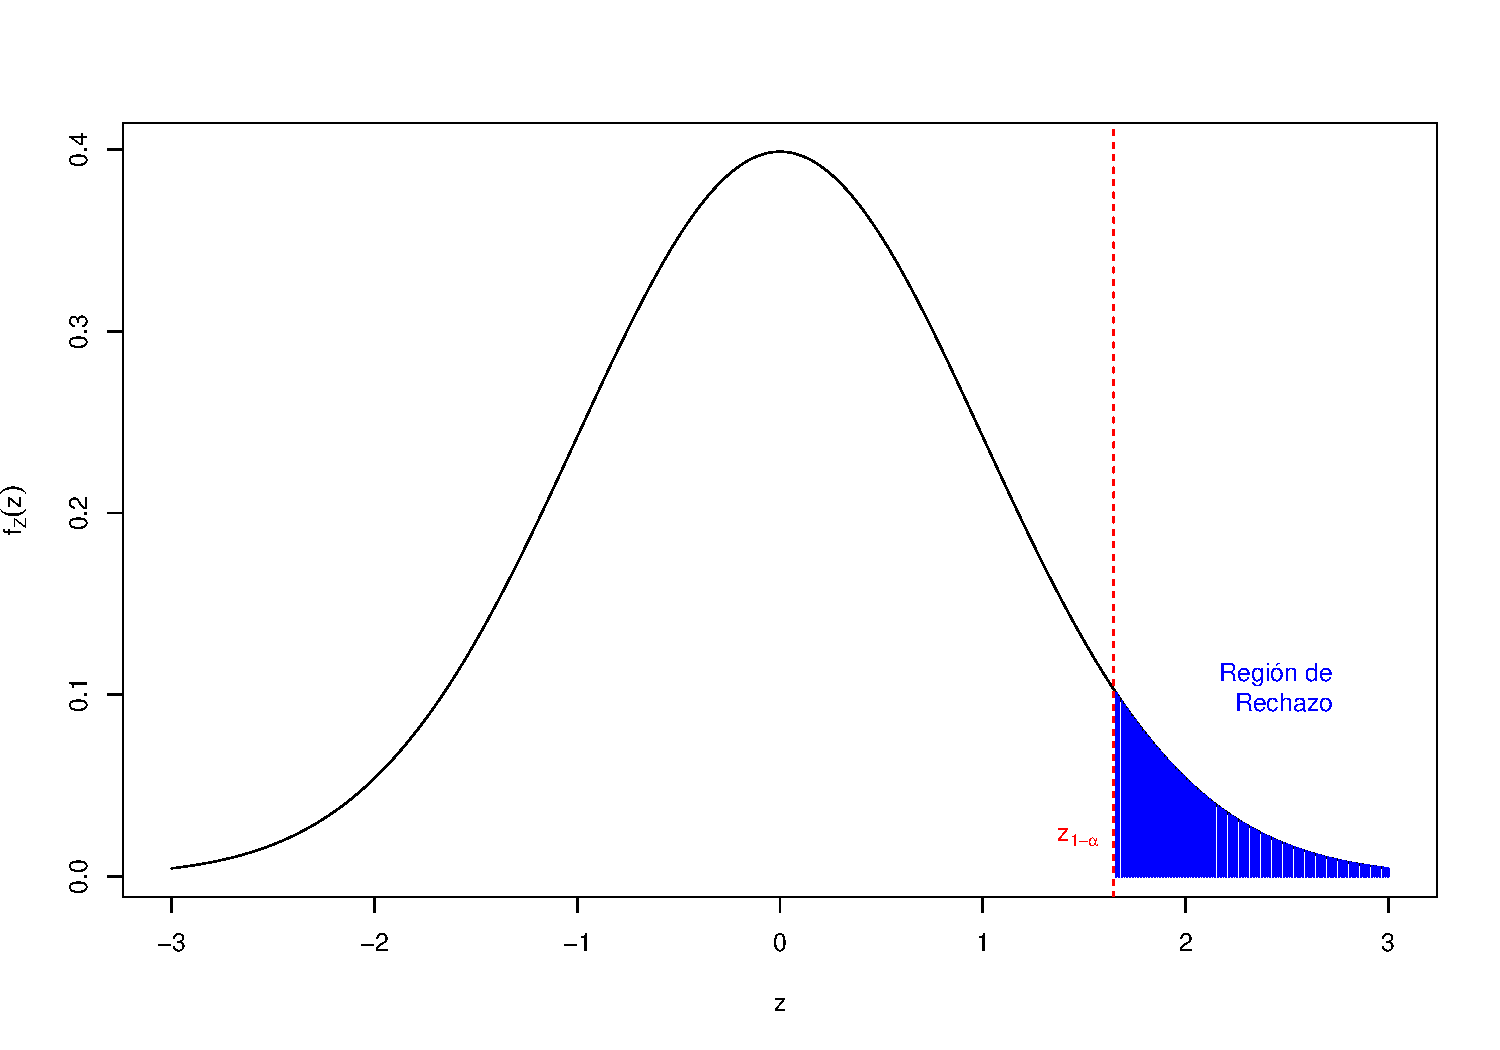
\includegraphics{contrastes_dos_muestras_files/figure-beamer/unnamed-chunk-1-1} \end{center}
\end{frame}

\begin{frame}{Contrastes de hipótesis para el parámetro \(\mu\) de una
variable normal con \(\sigma\) conocida}
\protect\hypertarget{contrastes-de-hipuxf3tesis-para-el-paruxe1metro-mu-de-una-variable-normal-con-sigma-conocida-5}{}
El contraste anterior tiene como:

\begin{itemize}[<+->]
\item
  \textbf{Estadístico de contraste}:
  \(Z=\dfrac{\overline{X}-\mu_0}{\frac{\sigma}{\sqrt{n}}}\).
\item
  \textbf{Región crítica}: \((z_{1-\alpha},\infty)\).
\item
  \textbf{Región de aceptación}: \((-\infty,z_{1-\alpha}]\).
\item
  \textbf{Regla de decisión}: rechazar \(H_0\) si \(Z>z_{1-\alpha}\).
\end{itemize}
\end{frame}

\begin{frame}{Contrastes de hipótesis para el parámetro \(\mu\) de una
variable normal con \(\sigma\) conocida}
\protect\hypertarget{contrastes-de-hipuxf3tesis-para-el-paruxe1metro-mu-de-una-variable-normal-con-sigma-conocida-6}{}
\begin{itemize}[<+->]
\item
  \textbf{Intervalo de confianza}: \[
  \begin{array}{l}
  Z< z_{1-\alpha}\Longleftrightarrow \dfrac{\overline{X}-\mu_0}{\frac{\sigma}{\sqrt{n}}}< z_{1-\alpha} 
  \Longleftrightarrow \mu_0> \overline{X}-z_{1-\alpha}\cdot\frac{\sigma}{\sqrt{n}}\\
  \qquad\quad\Longleftrightarrow \mu_0\in {\Big(\overline{X}-z_{1-\alpha}\cdot\frac{\sigma}{\sqrt{n}},\infty\Big)}
  \end{array}
  \]
\item
  \textbf{Regla de decisión II}: rechazar \(H_0\) si el \(\mu_0\)
  contrastado no pertenece al intervalo de confianza.
\end{itemize}
\end{frame}

\begin{frame}{Contrastes de hipótesis para el parámetro \(\mu\) de una
variable normal con \(\sigma\) conocida}
\protect\hypertarget{contrastes-de-hipuxf3tesis-para-el-paruxe1metro-mu-de-una-variable-normal-con-sigma-conocida-7}{}
\textbf{Ejercicio}

Sea \(X\) una población normal con \(\sigma=1.8\). Queremos hacer el
contraste \[
\left\{\begin{array}{l}
H_0:\mu=20\\ H_1:\mu>20
\end{array}
\right.
\] con un nivel de significación de \(0.05\).

Tomamos una m.a.s. de \(n=25\) observaciones y obtenemos
\(\overline{x}=20.25\).

¿Qué decidimos?
\end{frame}

\begin{frame}{Contrastes de hipótesis para el parámetro \(\mu\) de una
variable normal con \(\sigma\) conocida}
\protect\hypertarget{contrastes-de-hipuxf3tesis-para-el-paruxe1metro-mu-de-una-variable-normal-con-sigma-conocida-8}{}
Tenemos los siguientes valores: \(\alpha=0.05\), \(\sigma=1.8\),
\(n=25\), \(\overline{x}=20.25\).

El \textbf{Estadístico de contraste} valdrá
\(Z=\dfrac{\overline{X}-20}{\frac{1.8}{\sqrt{25}}}=0.694.\)

La \textbf{Región crítica} será \((z_{1-0.05},\infty)=(1.645,\infty)\).

\textbf{Decisión}: Como que \(0.694<1.645\), no pertenece a la región
crítica y por tanto no tenemos suficientes evidencias para rechazar
\(H_0\).

El \textbf{Intervalo de confianza} será: \[
\Big(\overline{X}-z_{1-\alpha}\cdot\frac{\sigma}{\sqrt{n}},\infty\Big)=(19.658,\infty)
\] \textbf{Decisión II}: Como \(\mu_0=20\) pertenece al intervalo de
confianza, no podemos rechazar \(H_0\).
\end{frame}

\begin{frame}{Contraste de hipótesis para a \(\mu\) de normal con
\(\sigma\) conocida}
\protect\hypertarget{contraste-de-hipuxf3tesis-para-a-mu-de-normal-con-sigma-conocida}{}
Sea \(X\) una v.a. \(N(\mu,\sigma)\) con \(\mu\) desconocida y
\(\sigma\) conocida

Sea \(X_1,\ldots,X_{n}\) una m.a.s. de \(X\) de tamaño \(n\)

Nos planteamos el contraste \[
\left\{\begin{array}{l}
H_0:\mu=\mu_0\\ H_1:\mu\ <\ \mu_0
\end{array}
\right.
\] donde vamos a rechazar \(H_0\) si
\(Z=\dfrac{\overline{X}-\mu_0}{{\sigma}/{\sqrt{n}}}\) es \emph{inferior
a} un cierto umbral, que determinaremos con \(\alpha\).
\end{frame}

\begin{frame}{Contraste de hipótesis para una media poblacional \(\mu\)
de una distribución normal con \(\sigma\) conocida}
\protect\hypertarget{contraste-de-hipuxf3tesis-para-una-media-poblacional-mu-de-una-distribuciuxf3n-normal-con-sigma-conocida}{}
Queremos que el \textbf{Error Tipo I} sea \(\alpha\): \[
\alpha  =P(\mbox{rechazar } H_0| H_0 \mbox{ cierta})
 =P(Z<\mbox{umbral })\Longrightarrow \mbox{umbral }=z_{\alpha},
\] por lo tanto, para que el nivel de significación del contraste Sea
\(\alpha\), la regla de rechazo tiene que ser \(Z<z_{\alpha}\).

La Región crítica es \((-\infty,z_{\alpha})\).

En resumen, \textbf{rechazamos \(H_0\)} si
\(\dfrac{\overline{X}-\mu_{0}}{\sigma/\sqrt{n}} < z_{\alpha}=-z_{1-\alpha}\).
\end{frame}

\begin{frame}{Contrastes de hipótesis para el parámetro \(\mu\) de una
variable normal con \(\sigma\) conocida}
\protect\hypertarget{contrastes-de-hipuxf3tesis-para-el-paruxe1metro-mu-de-una-variable-normal-con-sigma-conocida-9}{}
Gráfico de la región de rechazo. Las abscisas o coordenadas \(x\) de la
zona en azul serían los valores \(z\) para los que rechazaríamos la
hipótesis nula \(H_0\):

\begin{center}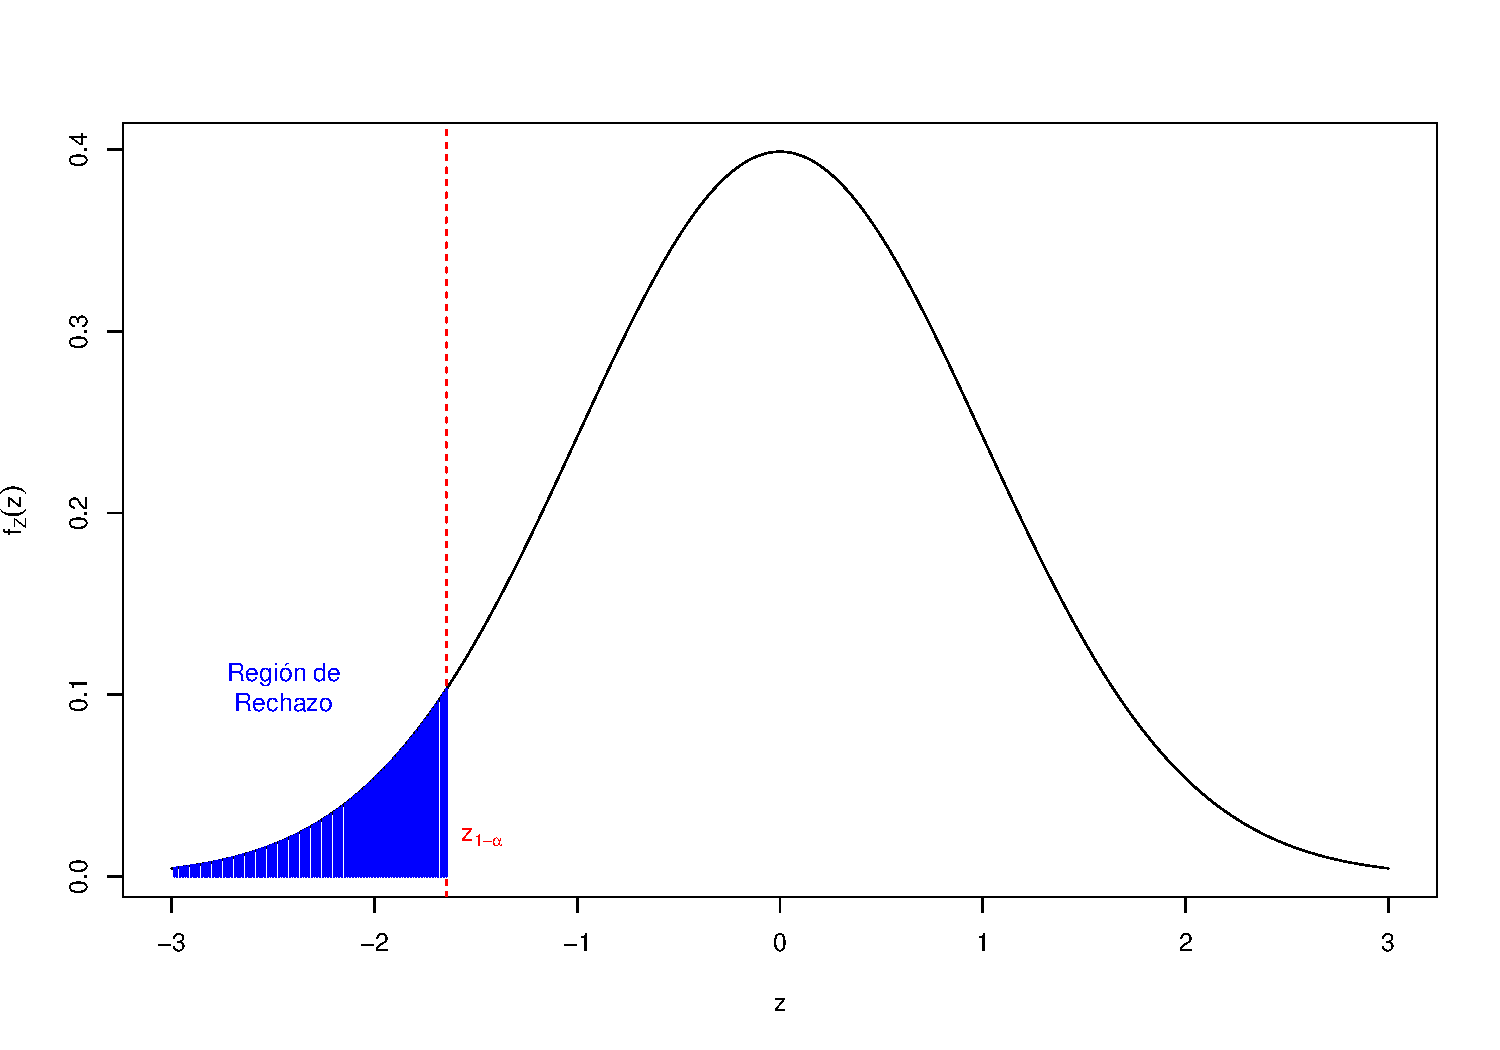
\includegraphics{contrastes_dos_muestras_files/figure-beamer/unnamed-chunk-2-1} \end{center}
\end{frame}

\begin{frame}{Contrastes de hipótesis para el parámetro \(\mu\) de una
variable normal con \(\sigma\) conocida}
\protect\hypertarget{contrastes-de-hipuxf3tesis-para-el-paruxe1metro-mu-de-una-variable-normal-con-sigma-conocida-10}{}
El contraste anterior tiene como:

\begin{itemize}[<+->]
\item
  \textbf{Estadístico de contraste}:
  \(Z=\dfrac{\overline{X}-\mu_0}{\frac{\sigma}{\sqrt{n}}}\).
\item
  \textbf{Región crítica}: \((-\infty,-z_{1-\alpha})\).
\item
  \textbf{Región de aceptación}: \([-z_{1-\alpha},\infty)\).
\item
  \textbf{Regla de decisión}: rechazar \(H_0\) si \(Z < -z_{1-\alpha}\).
\end{itemize}
\end{frame}

\begin{frame}{Contrastes de hipótesis para el parámetro \(\mu\) de una
variable normal con \(\sigma\) conocida}
\protect\hypertarget{contrastes-de-hipuxf3tesis-para-el-paruxe1metro-mu-de-una-variable-normal-con-sigma-conocida-11}{}
\begin{itemize}[<+->]
\item
  \textbf{Intervalo de confianza}: \[
  \begin{array}{l}
  Z> -z_{1-\alpha}\Longleftrightarrow \dfrac{\overline{X}-\mu_0}{\frac{\sigma}{\sqrt{n}}}> -z_{1-\alpha} 
  \Longleftrightarrow \mu_0< \overline{X}+z_{1-\alpha}\cdot\frac{\sigma}{\sqrt{n}}\\
  \qquad\quad\Longleftrightarrow \mu_0\in {\Big(-\infty,\overline{X}+z_{1-\alpha}\cdot\frac{\sigma}{\sqrt{n}}\Big)}
  \end{array}
  \]
\item
  \textbf{Regla de decisión II}: rechazar \(H_0\) si el \(\mu_0\)
  contrastado no pertenece al intervalo de confianza.
\end{itemize}
\end{frame}

\begin{frame}{Contraste de hipótesis para la media \(\mu\) de una
población normal con \(\sigma\) conocida}
\protect\hypertarget{contraste-de-hipuxf3tesis-para-la-media-mu-de-una-poblaciuxf3n-normal-con-sigma-conocida}{}
Sea \(X\) una v.a. \(N(\mu,\sigma)\) con \(\mu\) desconocida y
\(\sigma\) conocida

Sea \(X_1,\ldots,X_{n}\) una m.a.s. de \(X\) de tamaño \(n\)

Consideremos ahora el contraste \[
\left\{\begin{array}{l}
H_0:\mu=\mu_0\\ H_1:\mu\ \neq\ \mu_0
\end{array}
\right.
\]

Rechazar \(H_0\) si
\(Z=\dfrac{\overline{X}-\mu_0}{{\sigma}/{\sqrt{n}}}\) está a
\emph{bastante lejos de} de 0, y la determinaremos con el valor de
\(\alpha\)
\end{frame}

\begin{frame}{Contraste de hipótesis para la media \(\mu\) de una
población normal con \(\sigma\) conocida}
\protect\hypertarget{contraste-de-hipuxf3tesis-para-la-media-mu-de-una-poblaciuxf3n-normal-con-sigma-conocida-1}{}
Queremos como antes que el \textbf{Error Tipo I} sea \(\alpha\): \[
\begin{array}{rl}
\alpha & =P(\mbox{rechazar } H_0| H_0 \mbox{ cierta })
 =P(Z<-\mbox{umbral }\mbox{ o }Z>\mbox{umbral })\\
& =P(Z<-\mbox{umbral })\!+\!P(Z>\mbox{umbral })
 = 2P(Z>\mbox{umbral }) \\ &= 2(1-P(Z<\mbox{umbral }))
 \Longrightarrow P(Z<\mbox{umbral })=1-\dfrac{\alpha}2,\\
& \qquad \Longrightarrow \mbox{umbral }=z_{1-\frac{\alpha}2}.
\end{array}
\]
\end{frame}

\begin{frame}{Contraste de hipótesis para la media \(\mu\) de una
población normal con \(\sigma\) conocida}
\protect\hypertarget{contraste-de-hipuxf3tesis-para-la-media-mu-de-una-poblaciuxf3n-normal-con-sigma-conocida-2}{}
Ahora para que el nivel de significación del contraste sea \(\alpha\),
la \textbf{regla de rechazo} tiene que ser \[
Z<-z_{1-\frac{\alpha}2}=z_{\frac{\alpha}2}\mbox{ o }Z>z_{1-\frac{\alpha}2}.
\] La región crítica es
\((-\infty,z_{\frac\alpha2})\cup (z_{1-\frac{\alpha}2},\infty).\)
\end{frame}

\begin{frame}{Contraste de hipótesis para la media \(\mu\) de una
población normal con \(\sigma\) conocida}
\protect\hypertarget{contraste-de-hipuxf3tesis-para-la-media-mu-de-una-poblaciuxf3n-normal-con-sigma-conocida-3}{}
Gráfico de la región de rechazo. Las abscisas o coordenadas \(x\) de la
zona en azul serían los valores \(z\) para los que rechazaríamos la
hipótesis nula \(H_0\):

\begin{center}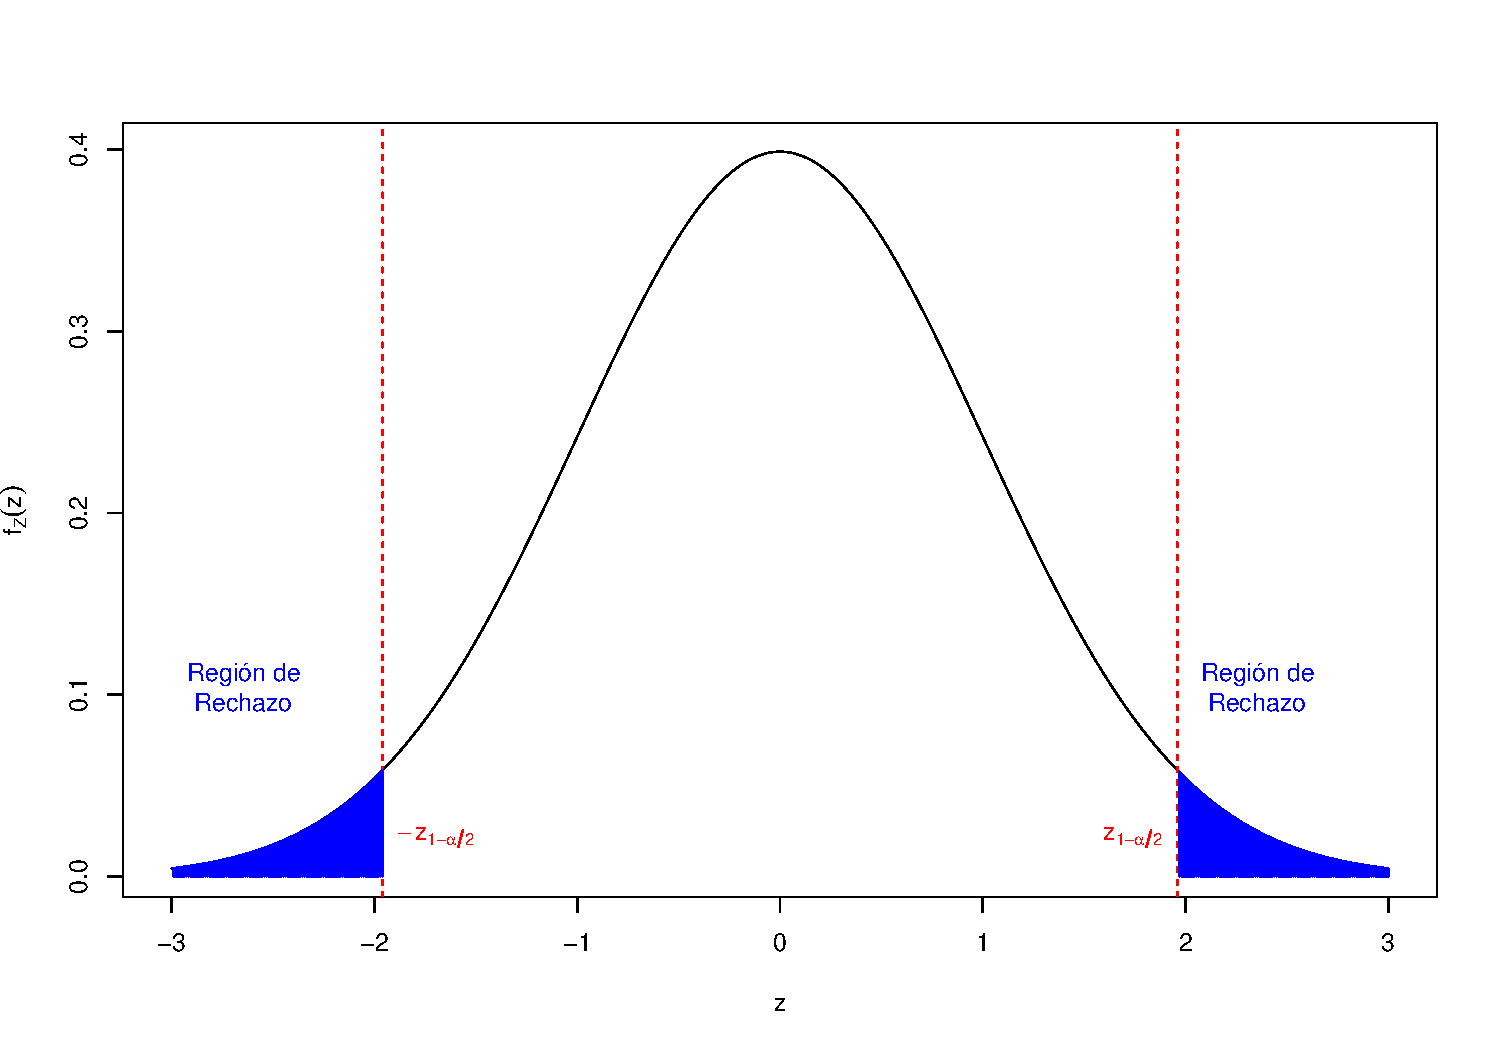
\includegraphics{contrastes_dos_muestras_files/figure-beamer/unnamed-chunk-3-1} \end{center}
\end{frame}

\begin{frame}{Contraste de hipótesis para la media \(\mu\) de una
población normal con \(\sigma\) conocida}
\protect\hypertarget{contraste-de-hipuxf3tesis-para-la-media-mu-de-una-poblaciuxf3n-normal-con-sigma-conocida-4}{}
Seguidamente, calculemos el \textbf{Intervalo de confianza} para el
contraste anterior: \[
\begin{array}{l}
-z_{1-\frac{\alpha}2} < Z < z_{1-\frac{\alpha}2}\Longleftrightarrow -z_{1-\frac{\alpha}2} < \dfrac{\overline{X}-\mu_0}{\frac{\sigma}{\sqrt{n}}}< z_{1-\frac{\alpha}2}\\
\qquad\Longleftrightarrow -z_{1-\frac{\alpha}2}\frac{\sigma}{\sqrt{n}}< \overline{X}-\mu_0< z_{1-\frac{\alpha}2}\frac{\sigma}{\sqrt{n}}\\\qquad \Longleftrightarrow \overline{X}-z_{1-\frac\alpha2}\frac{\sigma}{\sqrt{n}}< \mu_0< \overline{X}+z_{1-\frac{\alpha}2}\frac{\sigma}{\sqrt{n}} \\
\qquad\Longleftrightarrow\mu_0\in \Big(\overline{X}-z_{1-\frac\alpha2}\frac{\sigma}{\sqrt{n}},\overline{X}+z_{1-\frac{\alpha}2}\frac{\sigma}{\sqrt{n}}\Big)
   \end{array}
\]
\end{frame}

\begin{frame}{Contraste de hipótesis para la media \(\mu\) de una
población normal con \(\sigma\) conocida}
\protect\hypertarget{contraste-de-hipuxf3tesis-para-la-media-mu-de-una-poblaciuxf3n-normal-con-sigma-conocida-5}{}
\textbf{Ejercicio}

Sea \(X\) una población normal con \(\sigma=1.8\). Queremos realizar el
contraste \[
\left\{\begin{array}{l}
H_0:\mu=20\\ H_1:\mu\neq 20
\end{array}
\right.
\] con un nivel de significación de \(0.05\).

Tomamos una m.a.s. de \(n=25\) observaciones y obtenemos
\(\overline{x}=20.5\).

¿Qué decidimos?
\end{frame}

\begin{frame}{Contraste de hipótesis para la media \(\mu\) de una
población normal con \(\sigma\) conocida}
\protect\hypertarget{contraste-de-hipuxf3tesis-para-la-media-mu-de-una-poblaciuxf3n-normal-con-sigma-conocida-6}{}
Tenemos los valores siguientes: \(\alpha=0.05\), \(\sigma=1.8\),
\(n=25\), \(\overline{x}=20.5\).

El \textbf{Estadístico de contraste} vale
\(Z= \dfrac{\overline{X}-20}{\frac{1.8}{\sqrt{25}}}=1.389.\)

La \textbf{Región crítica} será:
\((-\infty,z_{0.025}[\cup ]z_{0.975},\infty)\)=\((-\infty,-1.96)\cup (1.96,\infty)\).

El \textbf{Intervalo de confianza} será:
\(\left(20.5-1.96 \frac{1.8}{\sqrt{25}}, 20.5+1.96 \frac{1.8}{\sqrt{25}}\right) = (19.794,21.206)\).

\textbf{Decisión}: No tenemos evidencias suficientes para rechazar
\(H_0\) ya que, por un lado, el estadístico de contraste no pertenece a
la región crítica y, por otro, el valor \(\mu_0 =20\) pertenece al
intervalo de confianza.
\end{frame}

\begin{frame}{El \(p\)-valor}
\protect\hypertarget{el-p-valor}{}
El \emph{\(p\)-valor} o \emph{valor crítico} (\(p\)-\emph{value}) de un
contraste es la probabilidad que, si \(H_0\) es verdadera, el
estadístico de contraste tome un valor tan extremo o más que el que se
ha observado.

Consideremos por ejemplo un contraste del tipo: \[
\left\{\begin{array}{l}
H_0:\mu=\mu_0\\ H_1:\mu\ >\ \mu_0.
\end{array}
\right.
\] Si el estadístico \(Z\) tiene el valor \(z_0\), el \(p\)-valor será:
\[
\mbox{$p$-valor}=P(Z\ \geq\ z_0).
\]
\end{frame}

\begin{frame}{El \(p\)-valor}
\protect\hypertarget{el-p-valor-1}{}
\begin{center}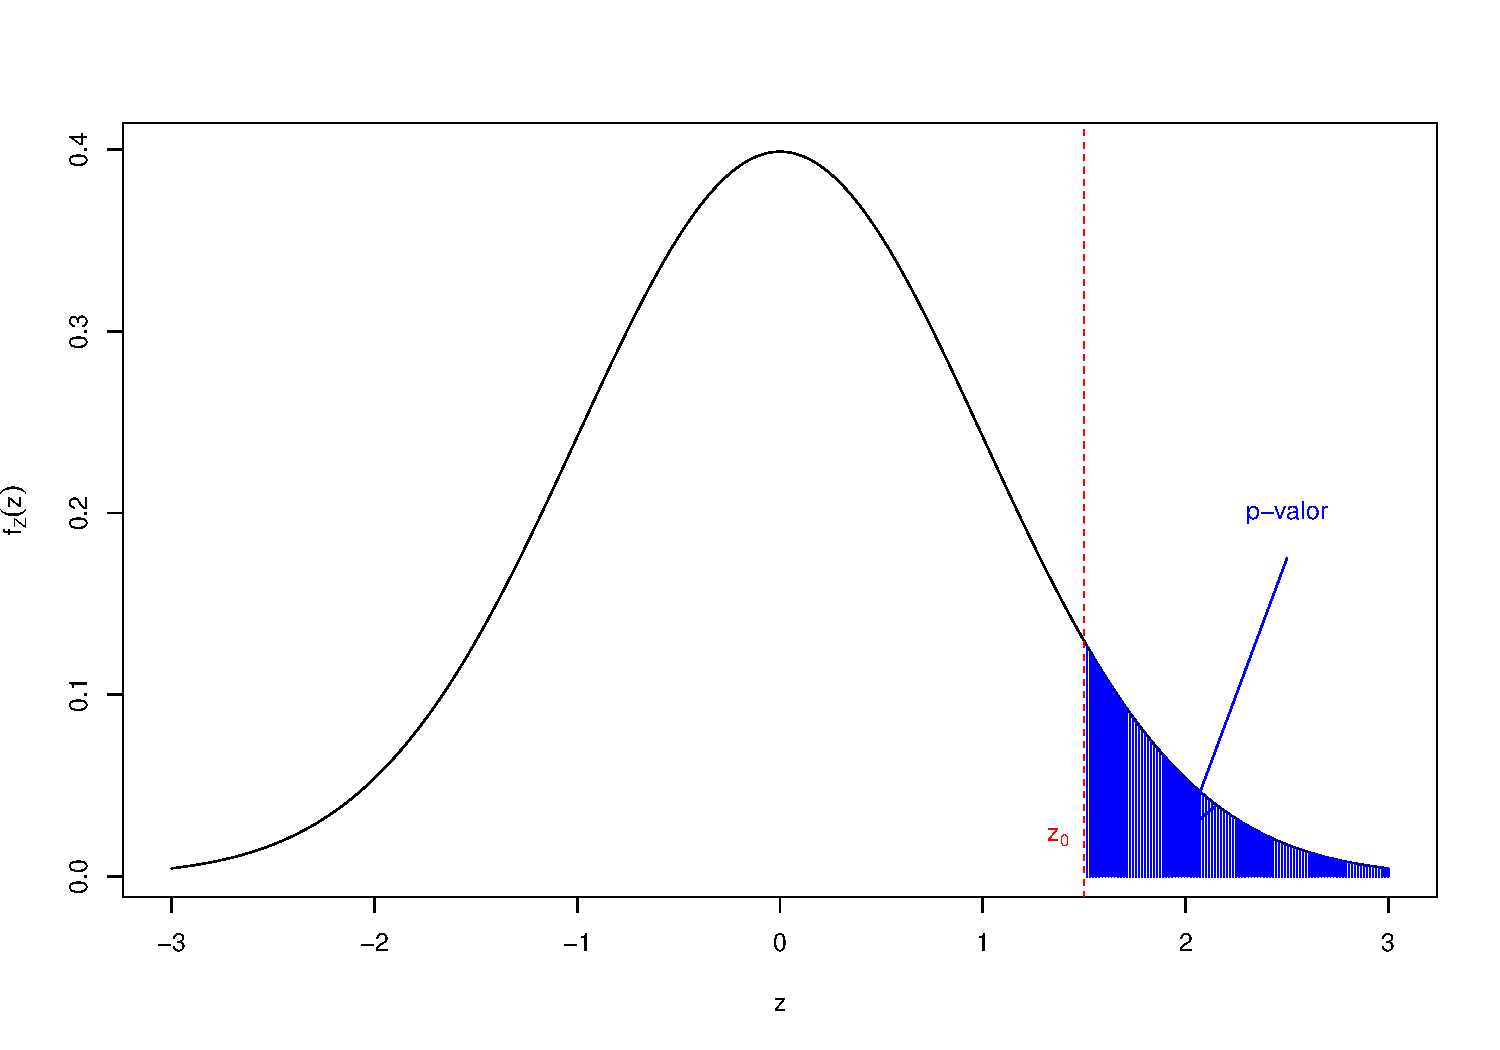
\includegraphics{contrastes_dos_muestras_files/figure-beamer/unnamed-chunk-4-1} \end{center}
\end{frame}

\begin{frame}{El \(p\)-valor}
\protect\hypertarget{el-p-valor-2}{}
Para el contraste:

\[
\left\{\begin{array}{l}
H_0:\mu=\mu_0\\ H_1:\mu\ <\ \mu_0.
\end{array}
\right.
\] Si el estadístico \(Z\) tiene el valor \(z_0\), el \(p\)-valor será:
\[
\mbox{$p$-valor}=P(Z\ \leq\ z_0).
\]
\end{frame}

\begin{frame}{El \(p\)-valor}
\protect\hypertarget{el-p-valor-3}{}
\begin{center}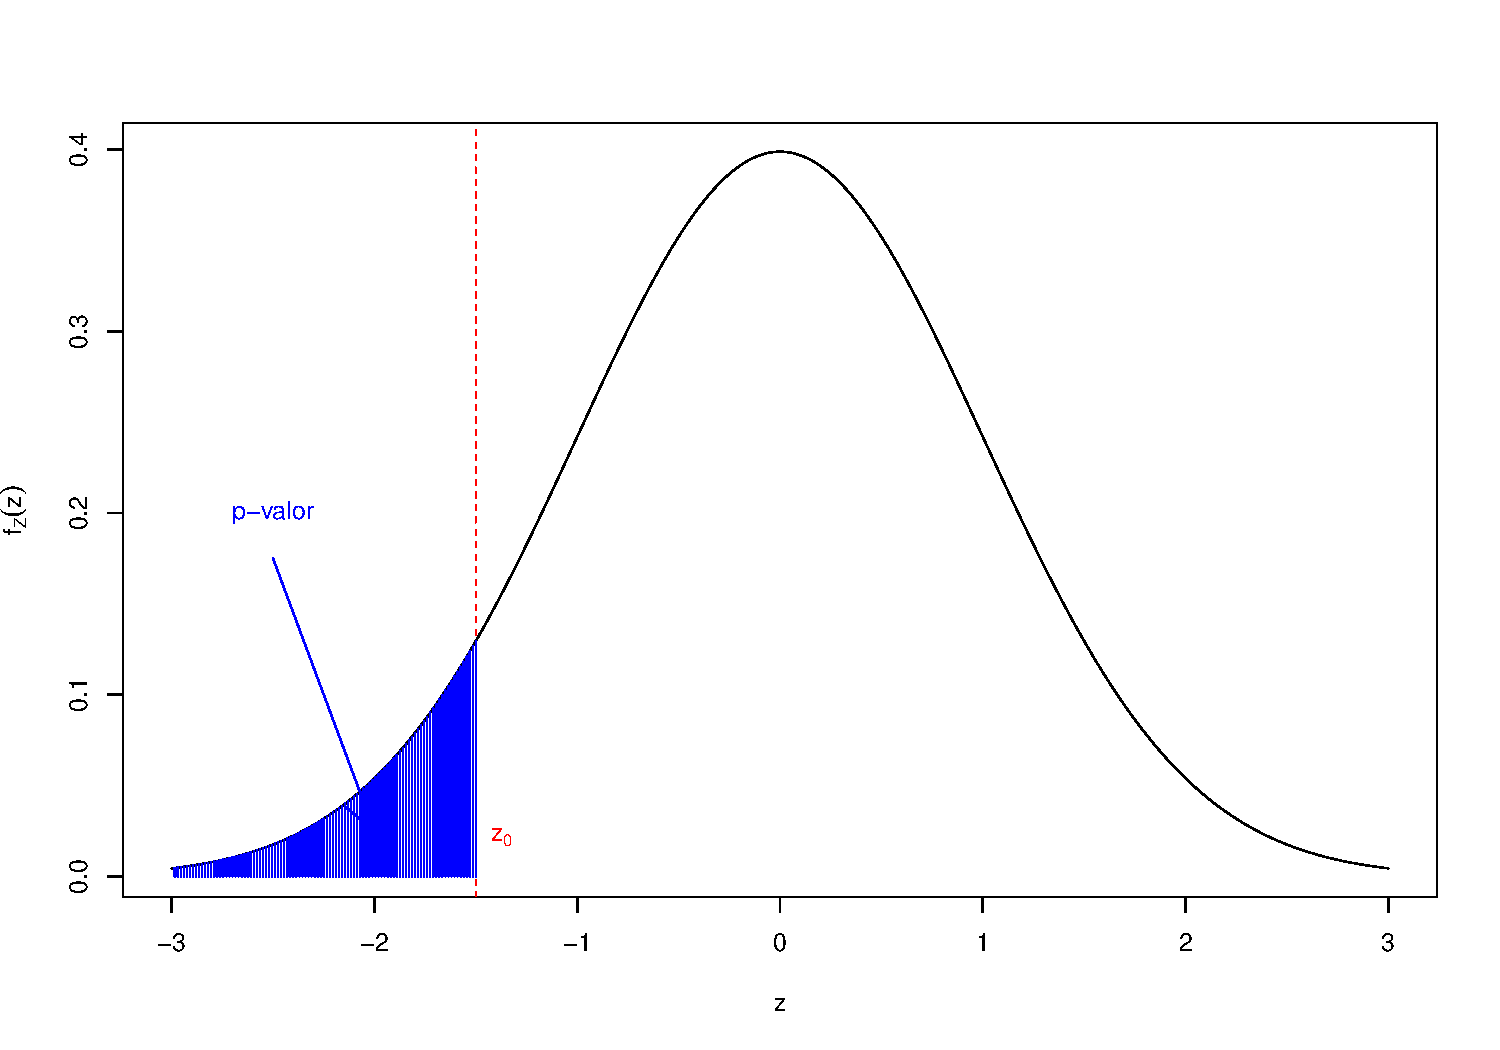
\includegraphics{contrastes_dos_muestras_files/figure-beamer/unnamed-chunk-5-1} \end{center}
\end{frame}

\begin{frame}{El \(p\)-valor}
\protect\hypertarget{el-p-valor-4}{}
Si ahora consideramos el contraste \[
\left\{\begin{array}{l}
H_0:\mu=\mu_0\\ H_1:\mu\ \neq\ \mu_0
\end{array}
\right.
\] y si el estadístico \(Z\) ha dado \(z_0\), el \(p\)-valor será: \[
\mbox{$p$-valor}  =2 \cdot \min\{P(Z \leq -|z_0|),P(Z \geq |z_0|)
  =2\cdot P(Z \geq |z_0|)
\]
\end{frame}

\begin{frame}{El \(p\)-valor}
\protect\hypertarget{el-p-valor-5}{}
\begin{center}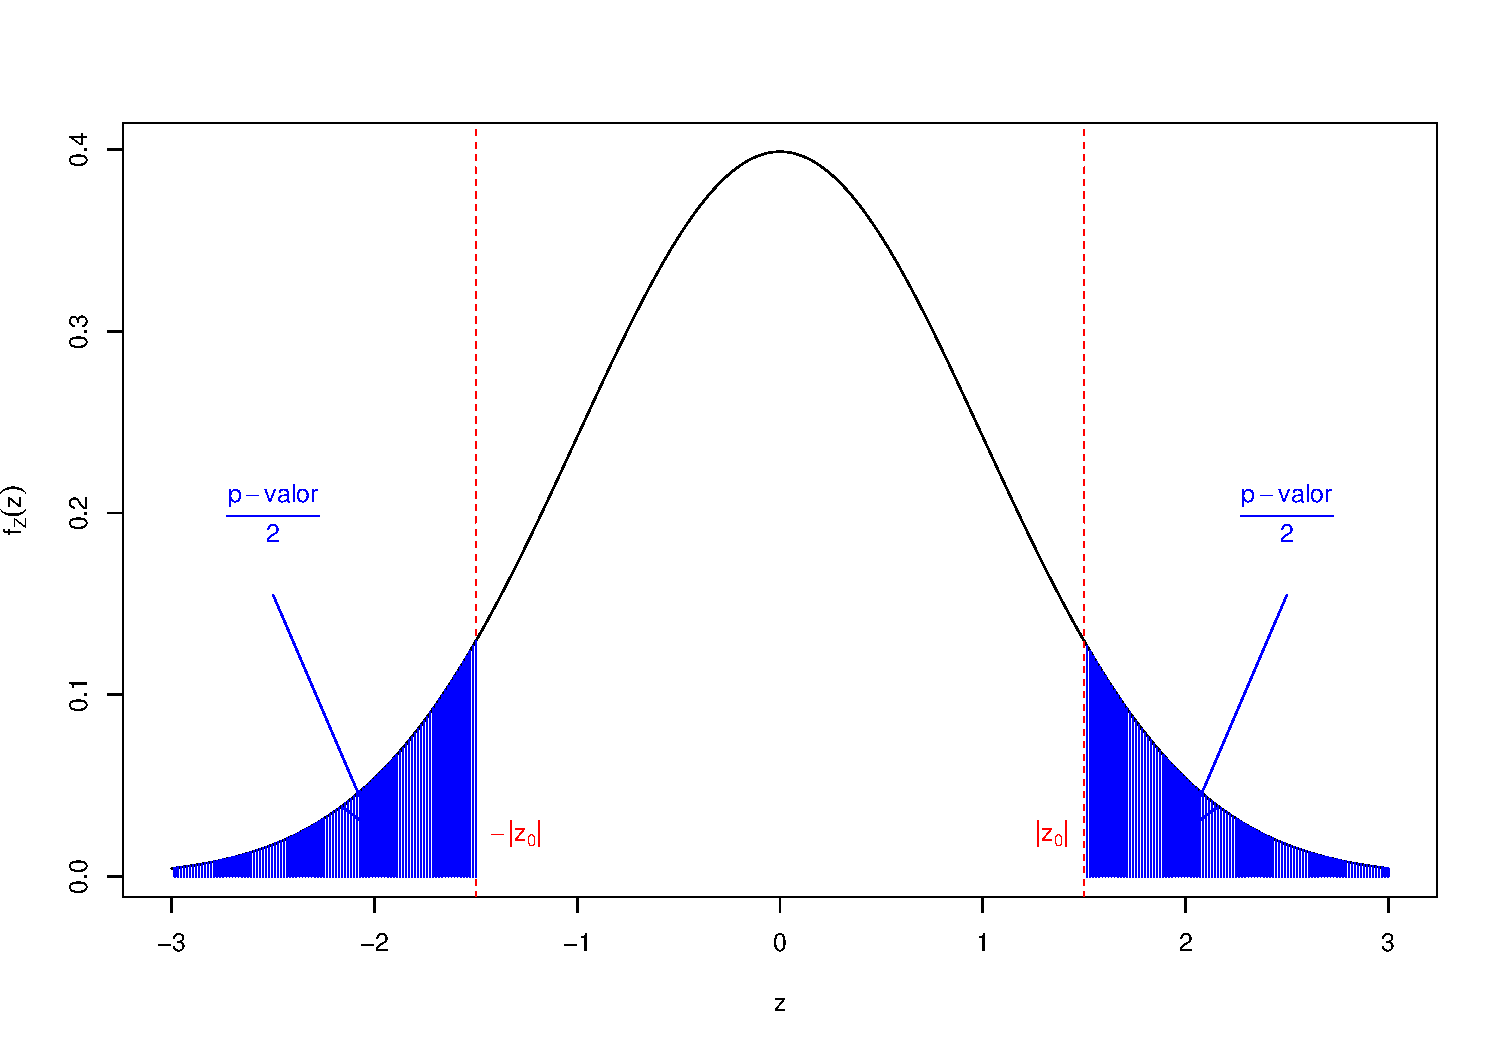
\includegraphics{contrastes_dos_muestras_files/figure-beamer/unnamed-chunk-6-1} \end{center}
\end{frame}

\begin{frame}{El \(p\)-valor}
\protect\hypertarget{el-p-valor-6}{}
El \emph{\(p\)-valor} o \emph{valor crítico} (\(p\)-\emph{value}) de un
contraste es la probabilidad que, si \(H_0\) es verdadera, el
estadístico de contraste tome un valor tan extremo o más que el que se
ha observado.

Es una \emph{medida inversa de la fuerza de las pruebas o evidencias que
hay en contra de \(H_1\)}: si \(H_0\) es verdadera, cuanto más pequeño
sea el \(p\)-valor, más improbable es observar lo que hemos observado.

En consecuencia, cuanto más pequeño sea el \(p\)-valor, con más fuerza
podemos rechazar \(H_0\).
\end{frame}

\begin{frame}{El \(p\)-valor}
\protect\hypertarget{el-p-valor-7}{}
Supongamos, por ejemplo, que hemos obtenido un \(p\)-valor de \(0.03\):

\begin{itemize}[<+->]
\item
  \emph{Significa} que la probabilidad de que, si \(H_0\) es verdadera,
  el estadístico de contraste tome un valor tan extremo o más que el que
  ha tomado, es 0.03 (\textbf{pequeño: evidencia de que \(H_0\) es
  falsa.})
\item
  \emph{No significa}:

  \begin{itemize}[<+->]
  \item
    La probabilidad que \(H_0\) Sea verdadera es \(0.03\)
  \item
    \(H_0\) es verdadera un 3\% de les veces
  \end{itemize}
\end{itemize}
\end{frame}

\begin{frame}{El \(p\)-valor}
\protect\hypertarget{el-p-valor-8}{}
Importante:

En un contraste con nivel de significación \(\alpha\),

\begin{itemize}[<+->]
\item
  rechazamos \(H_0\) si \(p\)-valor \(<\alpha\).
\item
  aceptamos \(H_0\) si \(\alpha\leq p\)-valor.
\end{itemize}
\end{frame}

\begin{frame}{El \(p\)-valor}
\protect\hypertarget{el-p-valor-9}{}
Si consideramos por ejemplo un contraste del tipo: \[
\left\{\begin{array}{l}
H_0:\mu=\mu_0\\ H_1:\mu> \mu_0
\end{array}
\right.
\]

y suponemos que el estadístico \(Z\) vale \(z_0\). El \(p\)-valor es
\(P(Z \geq z_0)\). Entonces:

\begin{itemize}[<+->]
\item
  Rechazamos \(H_0\) \(\Longleftrightarrow z_0>z_{1-\alpha},\),
\item
  O, dicho de otra forma,
  \[\mbox{$p$-valor}=P(Z \geq z_0)<P(Z\geq z_{1-\alpha})=1-(1-\alpha)=\alpha.\]
\end{itemize}
\end{frame}

\begin{frame}{El \(p\)-valor}
\protect\hypertarget{el-p-valor-10}{}
Si ahora consideramos un contraste del tipo: \[
\left\{\begin{array}{l}
H_0:\mu=\mu_0\\ H_1:\mu < \mu_0
\end{array}
\right.
\]

y suponemos que el estadístico \(Z\) vale \(z_0\). El \(p\)-valor es
\(P(Z \leq z_0)\). Entonces:

\begin{itemize}[<+->]
\item
  Rechazamos \(H_0\) \(\Longleftrightarrow z_0 < z_{\alpha},\)
\item
  O, dicho de otra forma,
  \[\mbox{$p$-valor}=P(Z \leq z_0) < P(Z\leq z_{\alpha})=\alpha.\]
\end{itemize}
\end{frame}

\begin{frame}{El \(p\)-valor}
\protect\hypertarget{el-p-valor-11}{}
Por último, supongamos que el contraste es del tipo: \[
\left\{\begin{array}{l}
H_0:\mu=\mu_0\\ H_1:\mu \neq \mu_0
\end{array}
\right.
\] y que el estadístico \(Z\) vale \(z_0>0\). El \(p\)-valor es
\(2P(Z \geq |z_0|)\). Entonces:

\begin{itemize}[<+->]
\item
  Rechazamos \(H_0 \Longleftrightarrow |z_0|>z_{1-\frac{\alpha}{2}}\),
\item
  O, dicho de otra forma, \[
  \mbox{$p$-valor}=2P(Z \geq |z_0|)<2P(Z\geq z_{1-\frac{\alpha}2})=2\left(1-\left(1-\frac{\alpha}2\right)\right)=\alpha.
  \]
\end{itemize}
\end{frame}

\begin{frame}{El \(p\)-valor}
\protect\hypertarget{el-p-valor-12}{}
El \emph{\(p\)-valor} de un contraste es:

\begin{itemize}[<+->]
\item
  El nivel de significación \(\alpha\) más pequeño para el que
  rechazamos la hipótesis nula.
\item
  El nivel de significación \(\alpha\) más grande para el que
  aceptaríamos la hipótesis nula.
\item
  La probabilidad mínima de error de Tipo I que permitimos si rechazamos
  la hipótesis nula con el valor del estadístico de contraste obtenido.
\item
  La probabilidad máxima de error de Tipo I que permitimos si aceptamos
  la hipótesis nula con el valor del estadístico de contraste obtenido.
\end{itemize}
\end{frame}

\begin{frame}[fragile]{El \(p\)-valor}
\protect\hypertarget{el-p-valor-13}{}
Importante:

Si no establecemos un nivel de significación \(\alpha\), entonces

\begin{itemize}[<+->]
\item
  Aceptamos \(H_0\) si el \(p\)-valor es ``grande'' (\(\geq 0.1\)).
\item
  Rechazamos \(H_0\) si el \(p\)-valor es ``pequeño'' (\(<0.05\)). En
  este caso, el \(p\)-valor es:

  \begin{itemize}[<+->]
  \tightlist
  \item
    \emph{Significativo} si es \(< 0.05\) (En \texttt{R}, se simboliza
    con un asterisco, \texttt{*}).
  \item
    \emph{Fuertemente significativo} si es \(<0.01\) (En \texttt{R}, se
    simboliza con dos asteriscos, \texttt{**}).
  \item
    \emph{Muy significativo} si es \(<0.001\) (En \texttt{R}, se
    simboliza con tres asteriscos, \texttt{***}).
  \end{itemize}
\end{itemize}
\end{frame}

\begin{frame}{El \(p\)-valor}
\protect\hypertarget{el-p-valor-14}{}
Si el \(p\)-valor está entre \(0.05\) y \(0.1\) y no tenemos nivel de
significación, se requieren estudios posteriores para tomar una
decisión.

Es la denominada \textbf{zona crepuscular}, o \emph{twilight zone}.
\end{frame}

\begin{frame}{Ejemplo}
\protect\hypertarget{ejemplo}{}
\textbf{Ejercicio}

Sea \(X\) una población normal con \(\sigma=1.8\). Queremos hacer el
contraste \[
\left\{\begin{array}{l}
H_0:\mu=20,\\ H_1:\mu>20.
\end{array}
\right.
\]

Tomamos una m.a.s. de \(n=25\) observaciones y obtenemos
\(\overline{x}=20.25\).

¿Qué decidimos?
\end{frame}

\begin{frame}{Ejemplo}
\protect\hypertarget{ejemplo-1}{}
Como no nos dan el nivel de significación \(\alpha\), calcularemos el
\(p\)-valor.

Si calculamos el \textbf{estadístico de contraste}, obtenemos
\(z_0= \dfrac{\overline{X}-20}{\frac{1.8}{\sqrt{25}}}=\dfrac{20.25-20}{\frac{1.8}{\sqrt{25}}}=0.694.\)

El \textbf{\(p\)-valor} valdrá: \(p =P(Z\geq 0.694)= 0.244 > 0.1\)
grande.

La \textbf{decisión} que tomamos por consiguiente es que no tenemos
evidencias suficientes para rechazar \(H_0\).
\end{frame}

\begin{frame}{Ejemplo}
\protect\hypertarget{ejemplo-2}{}
\textbf{Ejercicio}

Sea \(X\) una población normal con \(\sigma=1.8\). Queremos hacer el
contraste \[
\left\{\begin{array}{l}
H_0:\mu=20\\ H_1:\mu>20
\end{array}
\right.
\]

Tomamos una m.a.s. de \(n=25\) observaciones y obtenemos
\(\overline{x}=20.75\).

¿Qué decidimos?
\end{frame}

\begin{frame}{Ejemplo}
\protect\hypertarget{ejemplo-3}{}
El \textbf{estadístico de contraste} será
\(Z= \dfrac{\overline{X}-20}{\frac{1.8}{\sqrt{25}}}= \dfrac{20.75-20}{\frac{1.8}{\sqrt{25}}}=2.083.\)

El \textbf{\(p\)-valor} será: \(P(Z\geq 2.083)=0.019\) pequeño.

En este caso la \textbf{decisión} será rechazar \(H_0\) ya que tenemos
suficientes evidencias para hacerlo.
\end{frame}

\begin{frame}{Decisiones}
\protect\hypertarget{decisiones-4}{}
Si conocemos el \textbf{nivel de significación} \(\alpha\), la decisión
que tomemos en un contraste se puede basar en:

\begin{itemize}[<+->]
\item
  \textbf{la región crítica:} si el estadístico de contraste cae dentro
  de la \textbf{región crítica} para al nivel de significación
  \(\alpha\), rechazamos \(H_0\).
\item
  \textbf{el intervalo de confianza:} si el \textbf{parámetro
  poblacional} a contrastar cae dentro del \textbf{intervalo de
  confianza} para el nivel \((1-\alpha)\cdot 100\%\) de confianza,
  aceptamos \(H_0\).
\item
  \textbf{el \(p\)-valor:} si el \(p\)-valor es más pequeño que el nivel
  de significación \(\alpha\), rechazamos \(H_0\).
\end{itemize}
\end{frame}

\begin{frame}{Decisiones}
\protect\hypertarget{decisiones-5}{}
Si desconocemos el \textbf{nivel de significación} \(\alpha\), la
decisión que tomemos en un contraste se puede basar en:

\begin{itemize}[<+->]
\tightlist
\item
  \textbf{el \(p\)-valor:} Si el \(p\)-valor es pequeño, rechazamos
  \(H_0\), y si es grande, la aceptamos.
\end{itemize}
\end{frame}

\begin{frame}{El método de los \emph{seis} pasos (caso de conocer
\(\alpha\))}
\protect\hypertarget{el-muxe9todo-de-los-seis-pasos-caso-de-conocer-alpha}{}
\begin{enumerate}[<+->]
[1)]
\item
  Establecer la hipótesis nula \(H_0\) y la hipótesis alternativa
  \(H_1\).
\item
  Fijar un nivel de significación \(\alpha\).
\item
  Seleccionar el estadístico de contraste apropiado.
\item
  Calcular el valor del estadístico de contraste a partir de les datos
  muestrales.
\item
  Calcular el \(p\)-valor del contraste.
\item
  \textbf{Decisión:} rechazar \(H_0\) en favor de \(H_1\) si el
  \(p\)-valor es más pequeño que \(\alpha\); en caso contrario, aceptar
  \(H_0\).
\end{enumerate}
\end{frame}

\begin{frame}{El método de los \emph{cinco} pasos (caso de no conocer
\(\alpha\))}
\protect\hypertarget{el-muxe9todo-de-los-cinco-pasos-caso-de-no-conocer-alpha}{}
\begin{enumerate}[<+->]
[1)]
\item
  Establecer la hipótesis nula \(H_0\) y la hipótesis alternativa
  \(H_1\).
\item
  Seleccionar el estadístico de contraste apropiado.
\item
  Calcular el valor del estadístico de contraste a partir de los valores
  de la muestra.
\item
  Calcular el \(p\)-valor del contraste.
\item
  \textbf{Decisión:} rechazar \(H_0\) en favor de \(H_1\) si el
  \(p\)-valor es pequeño (\(<0.05\)), aceptar \(H_0\) si el \(p\)-valor
  es grande (\(\geq 0.1\)), y ampliar el estudio si el \(p\)-valor está
  entre 0.05 y 0.1.
\end{enumerate}
\end{frame}

\begin{frame}{Ejemplo}
\protect\hypertarget{ejemplo-4}{}
\textbf{Ejercicio}

Los años de vida de un router sigue aproximadamente una ley de
distribución normal con \(\sigma=0.89\) años.

Una muestra aleatoria de la duración de 100 aparatos ha dado una vida
media de 7.18 años.

Queremos decidir si la vida media en de estos routers es superior a 7
años: \[
\left\{\begin{array}{l}
H_0:\mu=7,\\ 
H_1:\mu>7.
\end{array}
\right.
\]
\end{frame}

\begin{frame}{Ejemplo suponiendo que conocemos \(\alpha=0.05\)}
\protect\hypertarget{ejemplo-suponiendo-que-conocemos-alpha0.05}{}
Tomamos un nivel de significación \(\alpha=0.05\).

EL estadístico de contraste es \[
z_0=\frac{\overline{X}-7}{0.89/\sqrt{100}}=\frac{\overline{X}-7}{0.0089}=\frac{7.18-7}{0.089}=2.022.
\] El \(p\)-valor es \(p=P(Z\geq 2.022)=0.022.\)

Como \(0.022<\alpha\), rechazamos \(H_0\).

Concluimos que tenemos suficientes evidencias para aceptar que la vida
media de los routers es superior a los 7 años: \(\mu>7\).
\end{frame}

\begin{frame}{Ejemplo suponiendo que conocemos \(\alpha=0.01\)}
\protect\hypertarget{ejemplo-suponiendo-que-conocemos-alpha0.01}{}
Supongamos ahora que tomamos un nivel de significación \(\alpha=0.01\).

Como el \(p\)-valor \(0.022>\alpha\), no podemos rechazar \(H_0\).

En este caso, concluimos que no tenemos evidencias suficientes para
rechazar que la vida media de los routers sea de 7 años o menor:
\(\mu\leq 7\).
\end{frame}

\begin{frame}{Ejemplo suponiendo que \textbf{no} conocemos \(\alpha\)}
\protect\hypertarget{ejemplo-suponiendo-que-no-conocemos-alpha}{}
Como el p-valor obtenido, \(0.022\), es pequeño (\(<0.05\)), rechazamos
\(H_0\).

Concluimos que tenemos suficientes evidencias para aceptar que la vida
media de los routers es superior a los 7 años: \(\mu>7\).
\end{frame}

\begin{frame}{Un último consejo}
\protect\hypertarget{un-uxfaltimo-consejo}{}
Como una regla recomendaríamos en un informe:

\begin{itemize}[<+->]
\item
  \emph{Si conocemos \(\alpha\),} encontrar el \(p\)-valor y el
  intervalo de confianza del contraste para \(\alpha\) dado (nivel de
  confianza \((1-\alpha)\cdot 100\%\)).
\item
  \emph{Si no tenemos fijado (no conocemos) \(\alpha\),} encontrar el
  \(p\)-valor, y el intervalo de confianza del contraste al nivel de
  confianza \(95\%\).
\end{itemize}
\end{frame}

\begin{frame}{Contrastes de hipótesis para el parámetro \(\mu\) de una
variable normal con \(\sigma\) desconocida}
\protect\hypertarget{contrastes-de-hipuxf3tesis-para-el-paruxe1metro-mu-de-una-variable-normal-con-sigma-desconocida}{}
\end{frame}

\begin{frame}{Contraste para \(\mu\) cuando \(n\) es grande: Z-test}
\protect\hypertarget{contraste-para-mu-cuando-n-es-grande-z-test}{}
Si el tamaño \(n\) de la muestra es grande (pongamos \(n\geq 40\)),
podemos aplicar las reglas anteriores aunque la población no sea normal.

Si además \(\sigma\) es desconocida, ésta se puede sustituir por la
desviación típica muestral \(\widetilde{S}_X\) en la expresión de \(Z\):
\[
Z=\frac{\overline{X}-\mu_0}
{\frac{\widetilde{S}_X}{\sqrt{n}}}
\]
\end{frame}

\begin{frame}{Ejemplo}
\protect\hypertarget{ejemplo-5}{}
\textbf{Ejemplo}

Una organización ecologista afirma que el peso medio de los individuos
adultos de una especie marina ha disminuido drásticamente.

Se sabe por los datos históricos que el peso medio poblacional era de
460 g.

Una muestra aleatoria de 40 individuos de esta especie ha dado una media
muestral de 420 g. y una desviación típica muestral de 119 g.

Con estos datos, ¿podemos afirmar con un nivel de significación del 5\%
que el peso mediano es inferior a 460 g?
\end{frame}

\begin{frame}{Ejemplo}
\protect\hypertarget{ejemplo-6}{}
\textbf{Ejemplo}

El contraste que nos planteamos es el siguiente:
\[\left\{\begin{array}{l}
H_0:\mu=460,\\
H_1:\mu<460,
\end{array}
\right.\] donde \(\mu\) representa el peso medio de todos los individuos
de la especie.

Consideramos un \textbf{nivel de significación} \(\alpha=0.05\).

Podemos usar como \textbf{estadístico de contraste}, como \(n=40\) es
grande, la expresión: \[
Z=\frac{\overline{X}-\mu_0}{{\widetilde{S}_X}/{\sqrt{n}}},
\] cuyo valor es: \(z_0=\dfrac{420-460}{{119}/{\sqrt{40}}}=-2.126.\)
\end{frame}

\begin{frame}{Ejemplo}
\protect\hypertarget{ejemplo-7}{}
\textbf{Ejemplo}

El \textbf{\(p\)-valor} será: \[
P(Z\leq -2.126)=
0.017.
\] Decisión: como \(\alpha>p\)-valor, rechazamos (al nivel de
significación \(\alpha=0.05\)) que el peso medio sea de \(460\) g.
(\(H_0\)) en contra que sea menor de \(460\) g. (\(H_1\)).

Concluimos que tenemos suficientes evidencias para afirmar que el peso
medio es menor que \(460\) g. y por tanto, ha menguado en los últimos
años.
\end{frame}

\begin{frame}{Ejemplo}
\protect\hypertarget{ejemplo-8}{}
El \textbf{intervalo de confianza} será: \[
\left(-\infty, \overline{X}-z_{\alpha}\cdot \frac{\widetilde{S}_X}{\sqrt{n}}\right)=]-\infty,450.949].
\]

Informe: el \textbf{\(p\)-valor} de este contraste es \(0.017\), y el
intervalo de confianza al nivel de significación \(\alpha=0.05\) para la
media poblacional \(\mu\) es \(]-\infty,450.949]\).

Como \(460\not\in (-\infty,450.949)\), hay evidencia significativa para
rechazar la hipótesis nula en favor de \(\mu<460\).
\end{frame}

\begin{frame}{Contraste para \(\mu\) de normal con \(\sigma\)
desconocida: T-test}
\protect\hypertarget{contraste-para-mu-de-normal-con-sigma-desconocida-t-test}{}
Las reglas de decisión son similares al caso con \(\sigma\) conocida,
excepto que ahora \textbf{sustituimos \(\sigma\) por
\(\widetilde{S}_X\)} y empleamos la distribución \(t\) de Student.

Recordemos que si \(X_1,\ldots,X_n\) es una m.a.s. de una población
normal \(X\) con mediana \(\mu_0\), la variable
\(T= \frac{\overline{X}-\mu_0}{\frac{\widetilde{S}_X}{\sqrt{n}}}\) sigue
una distribución t de Student con \(n-1\) grados de libertad.

Los \(p\)-valores se calculan con esta distribución.
\end{frame}

\begin{frame}{Contraste de \(\mu\) de normal con \(\sigma\) desconocida:
T-test}
\protect\hypertarget{contraste-de-mu-de-normal-con-sigma-desconocida-t-test}{}
Condiciones: supongamos que disponemos de una m.a.s. de tamaño \(n\) de
una población \(N(\mu,\sigma)\) con \(\mu\) y \(\sigma\) desconocidas.

Nos planteamos los contrastes siguientes:

\(\left\{\begin{array}{l} H_0:\mu=\mu_0 \quad (\mbox{ o } H_0:\mu\leq \mu_0)\\ H_1:\mu>\mu_0 \end{array} \right.\)

\(\left\{\begin{array}{l} H_0:\mu=\mu_0 \quad (\mbox{ o } H_0:\mu\geq \mu_0)\\ H_1:\mu<\mu_0 \end{array} \right.\)

\(\left\{\begin{array}{l} H_0:\mu=\mu_0 \\ H_1:\mu \neq \mu_0 \end{array} \right.\)
\end{frame}

\begin{frame}{Contraste de \(\mu\) de normal con \(\sigma\) desconocida:
T-test}
\protect\hypertarget{contraste-de-mu-de-normal-con-sigma-desconocida-t-test-1}{}
Para los contrastes anteriores, usaremos como \textbf{estadístico de
contraste}: \[
T= \frac{\overline{X}-\mu_0}{\frac{\widetilde{S}_X}{\sqrt{n}}}
\] y calcularemos su valor \(t_0\) sobre la muestra.
\end{frame}

\begin{frame}{Contraste de \(\mu\) de normal con \(\sigma\) desconocida:
T-test}
\protect\hypertarget{contraste-de-mu-de-normal-con-sigma-desconocida-t-test-2}{}
Los \textbf{p-valores} serán los siguientes:

\(p\)-valor: \(P(t_{n-1}\geq t_0)\).

\(p\)-valor: \(P(t_{n-1}\leq t_0)\).

\(p\)-valor: \(2P(t_{n-1}\geq |t_0|)\).
\end{frame}

\begin{frame}{Ejemplo}
\protect\hypertarget{ejemplo-9}{}
\textbf{Ejercicio}

Se espera que el nivel de colesterol en plasma de unos enfermos bajo un
determinado tratamiento se distribuya normalmente con media 220 mg/dl.

Se toma una muestra de 9 enfermos, y se miden sus niveles: \[ 
203, 229, 215, 220, 223, 233, 208, 228, 209.
\]

Contrastar la hipótesis que esta muestra efectivamente proviene de una
población con media 220 mg/dl.
\end{frame}

\begin{frame}{Ejemplo}
\protect\hypertarget{ejemplo-10}{}
El contraste planteado es el siguiente: \[\left\{\begin{array}{l}
H_0:\mu=220,\\
H_1:\mu\neq 220,
\end{array}
\right.\] donde \(\mu\) representa la media del colesterol en plasma de
la población.

Bajo estas condiciones (población normal, \(\sigma\) desconocida,
muestra pequeña de \(n=9\)) usaremos como \textbf{estadístico de
contraste}: \(T= \frac{\overline{X}-\mu_0}{{\widetilde{S}_X}/{\sqrt9}}\)
cuya distribución es \(t_8\).
\end{frame}

\begin{frame}[fragile]{Ejemplo}
\protect\hypertarget{ejemplo-11}{}
El valor de dicho estadístico será:

\begin{Shaded}
\begin{Highlighting}[]
\NormalTok{colesterol=}\KeywordTok{c}\NormalTok{(}\DecValTok{203}\NormalTok{,}\DecValTok{229}\NormalTok{,}\DecValTok{215}\NormalTok{,}\DecValTok{220}\NormalTok{,}\DecValTok{223}\NormalTok{,}\DecValTok{233}\NormalTok{,}\DecValTok{208}\NormalTok{,}\DecValTok{228}\NormalTok{,}\DecValTok{209}\NormalTok{)}
\NormalTok{media.muestral =}\StringTok{ }\KeywordTok{mean}\NormalTok{(colesterol)}
\NormalTok{desv.típica.muestral =}\StringTok{ }\KeywordTok{sd}\NormalTok{(colesterol)}
\NormalTok{(estadístico}\DataTypeTok{.contraste =}\NormalTok{ (media.muestral}\DecValTok{{-}220}\NormalTok{)}\OperatorTok{/}
\StringTok{    }\NormalTok{(desv.típica.muestral}\OperatorTok{/}\KeywordTok{sqrt}\NormalTok{(}\KeywordTok{length}\NormalTok{(colesterol))))}
\end{Highlighting}
\end{Shaded}

\begin{verbatim}
## [1] -0.3800915
\end{verbatim}
\end{frame}

\begin{frame}[fragile]{Ejemplo}
\protect\hypertarget{ejemplo-12}{}
El \textbf{p-valor} del contraste será:

\begin{Shaded}
\begin{Highlighting}[]
\NormalTok{(}\DataTypeTok{p=}\KeywordTok{round}\NormalTok{(}\DecValTok{2}\OperatorTok{*}\KeywordTok{pt}\NormalTok{(}\KeywordTok{abs}\NormalTok{(estadístico.contraste),}\DataTypeTok{lower.tail=}\OtherTok{FALSE}\NormalTok{,}\DataTypeTok{df=}\DecValTok{8}\NormalTok{),}\DecValTok{4}\NormalTok{))}
\end{Highlighting}
\end{Shaded}

\begin{verbatim}
## [1] 0.7138
\end{verbatim}

Decisión: Como que el \(p\)-valor es muy grande, no podemos rechazar que
el nivel mediano de colesterol en plasma sea igual a 220 mg/dl.

Por tanto, aceptamos que el nivel de colesterol en plasma en esta
población tiene media 220 mg/dl.
\end{frame}

\begin{frame}{Ejemplo}
\protect\hypertarget{ejemplo-13}{}
El \textbf{intervalo de confianza} al 95\% será: \[
\begin{array}{rl}
\left(\overline{X}-t_{8,0.975}\frac{\widetilde{S}_X}{\sqrt{n}},\ \overline{X}+t_{8,0.975}\frac{\widetilde{S}_X}{\sqrt{n}}\right) & =\left(218.667-2.306\cdot \frac{10.524}{\sqrt{9}},218.667+2.306\cdot \frac{10.524}{\sqrt{9}}\right)\\ & =(210.577,226.756)
\end{array}
\]

Informe: El \(p\)-valor de este contraste es \(0.7138\) y el intervalo
de confianza del \(95\%\) para el nivel medio de colesterol \(\mu\) es
\((210.577,226.756)\).

Como el p-valor es grande y \(220\in (210.577,226.756)\), no hay
evidencia que nos permita rechazar que \(\mu=220\).
\end{frame}

\begin{frame}[fragile]{Contraste de \(\mu\) de normal con \(\sigma\)
desconocida en \texttt{R}: función \texttt{t.test}}
\protect\hypertarget{contraste-de-mu-de-normal-con-sigma-desconocida-en-r-funciuxf3n-t.test}{}
La sintaxis básica de la función \texttt{t.test} es

\begin{Shaded}
\begin{Highlighting}[]
\KeywordTok{t.test}\NormalTok{(x, y, }\DataTypeTok{mu=}\NormalTok{..., }\DataTypeTok{alternative=}\NormalTok{..., }\DataTypeTok{conf.level=}\NormalTok{..., }\DataTypeTok{paired=}\NormalTok{..., }
       \DataTypeTok{var.equal=}\NormalTok{..., }\DataTypeTok{na.omit=}\NormalTok{...)}
\end{Highlighting}
\end{Shaded}

donde los parámetros necesarios para realizar un contraste de una
muestra son los siguientes:

\begin{itemize}[<+->]
\item
  \texttt{x} es el vector de datos que forma la muestra que analizamos.
\item
  \texttt{mu} es el valor \(\mu_0\) de la hipótesis nula:
  \(H_0: \mu=\mu_0\).
\end{itemize}
\end{frame}

\begin{frame}[fragile]{Contraste de \(\mu\) de normal con \(\sigma\)
desconocida en \texttt{R}: función \texttt{t.test}}
\protect\hypertarget{contraste-de-mu-de-normal-con-sigma-desconocida-en-r-funciuxf3n-t.test-1}{}
\begin{itemize}[<+->]
\item
  El parámetro \texttt{alternative} puede tomar tres valores:
  \texttt{"two.sided"}, para contrastes bilaterales, y \texttt{"less"} y
  \texttt{"greater"}, para contrastes unilaterales. En esta función, y
  en todas las que explicamos en esta lección, su valor por defecto, que
  no hace falta especificar, es \texttt{"two.sided"}. El significado de
  estos valores depende del tipo de test que efectuemos:
\item
  \texttt{"two.sided"} representa la hipótesis alternativa
  \(H_1: \mu\neq \mu_0\), \texttt{"less"} corresponde a
  \(H_1: \mu< \mu_0\), y \texttt{"greater"} corresponde a
  \(H_1: \mu> \mu_0\).
\item
  El valor del parámetro \texttt{conf.level} es el nivel de confianza
  \(1-\alpha\). Su valor por defecto es 0.95, que corresponde a un nivel
  de confianza del 95\%, es decir, a un nivel de significación
  \(\alpha=0.05\).
\end{itemize}
\end{frame}

\begin{frame}[fragile]{Contraste de \(\mu\) de normal con \(\sigma\)
desconocida en \texttt{R}: función \texttt{t.test}}
\protect\hypertarget{contraste-de-mu-de-normal-con-sigma-desconocida-en-r-funciuxf3n-t.test-2}{}
\begin{itemize}[<+->]
\item
  El parámetro \texttt{na.action} sirve para especificar qué queremos
  hacer con los valores NA. Es un parámetro genérico que se puede usar
  en casi todas las funciones de estadística inferencial y análisis de
  datos. Sus valores más útiles son:

  \begin{itemize}[<+->]
  \item
    \texttt{na.omit}, su valor por defecto, elimina las entradas NA de
    los vectores (o los pares que contengan algún NA, en el caso de
    muestras emparejadas). Por ahora, esta opción por defecto es la
    adecuada, por lo que no hace falta usar este parámetro, pero
    conviene saber que hay alternativas.
  \item
    \texttt{na.fail} hace que la ejecución pare si hay algún NA en los
    vectores.
  \item
    \texttt{na.pass} no hace nada con los NA y permite que las
    operaciones internas de la función sigan su curso y los manejen como
    les corresponda.
  \end{itemize}
\end{itemize}
\end{frame}

\begin{frame}[fragile]{Contraste de \(\mu\) de normal con \(\sigma\)
desconocida en \texttt{R}: función \texttt{t.test}}
\protect\hypertarget{contraste-de-mu-de-normal-con-sigma-desconocida-en-r-funciuxf3n-t.test-3}{}
El ejemplo anterior se resolvería de la forma siguiente:

\begin{Shaded}
\begin{Highlighting}[]
\KeywordTok{t.test}\NormalTok{(colesterol,}\DataTypeTok{mu=}\DecValTok{220}\NormalTok{,}\DataTypeTok{alternative=}\StringTok{"two.sided"}\NormalTok{,}\DataTypeTok{conf.level=}\FloatTok{0.95}\NormalTok{)   }
\end{Highlighting}
\end{Shaded}

\begin{verbatim}
## 
##  One Sample t-test
## 
## data:  colesterol
## t = -0.38009, df = 8, p-value = 0.7138
## alternative hypothesis: true mean is not equal to 220
## 95 percent confidence interval:
##  210.5774 226.7560
## sample estimates:
## mean of x 
##  218.6667
\end{verbatim}
\end{frame}

\begin{frame}[fragile]{Contraste de \(\mu\) de normal con \(\sigma\)
desconocida en \texttt{R}: función \texttt{t.test}}
\protect\hypertarget{contraste-de-mu-de-normal-con-sigma-desconocida-en-r-funciuxf3n-t.test-4}{}
\textbf{Ejercicio}

Veamos si, dada una muestra de tamaño 40 de flores de la tabla de datos
iris, podemos considerar que la media de la longitud del sépalo es mayor
que \(5.7\).

Para ello, primero obtenemos la muestra correspondiente fijando la
semilla de aleatoriedad:

\begin{Shaded}
\begin{Highlighting}[]
\KeywordTok{set.seed}\NormalTok{(}\DecValTok{230}\NormalTok{)}
\NormalTok{flores.elegidas=}\KeywordTok{sample}\NormalTok{(}\DecValTok{1}\OperatorTok{:}\DecValTok{150}\NormalTok{,}\DecValTok{40}\NormalTok{,}\DataTypeTok{replace=}\OtherTok{TRUE}\NormalTok{)}
\end{Highlighting}
\end{Shaded}

Seguidamente, hallamos las longitudes del sépalo de las flores de la
muestra:

\begin{Shaded}
\begin{Highlighting}[]
\NormalTok{(long.sépalo}\DataTypeTok{.muestra=}\NormalTok{iris[flores.elegidas,]}\OperatorTok{$}\NormalTok{Sepal.Length)}
\end{Highlighting}
\end{Shaded}

\begin{verbatim}
##  [1] 5.0 4.9 6.0 4.6 4.7 5.1 5.8 4.4 4.6 7.0 7.7 4.8 4.9 7.2 6.5 4.8 7.7 6.2 5.1
## [20] 6.8 7.2 5.0 6.7 6.9 4.6 5.7 6.4 6.1 6.4 4.7 5.0 7.7 6.2 5.0 5.1 4.9 6.3 5.0
## [39] 5.6 5.2
\end{verbatim}
\end{frame}

\begin{frame}[fragile]{Contraste de \(\mu\) de normal con \(\sigma\)
desconocida en \texttt{R}: función \texttt{t.test}}
\protect\hypertarget{contraste-de-mu-de-normal-con-sigma-desconocida-en-r-funciuxf3n-t.test-5}{}
Por último, realizamos el contraste requerido:

\begin{Shaded}
\begin{Highlighting}[]
\KeywordTok{t.test}\NormalTok{(long.sépalo.muestra,}\DataTypeTok{mu=}\FloatTok{5.7}\NormalTok{,}\DataTypeTok{alternative =} \StringTok{"greater"}\NormalTok{)}
\end{Highlighting}
\end{Shaded}

\begin{verbatim}
## 
##  One Sample t-test
## 
## data:  long.sépalo.muestra
## t = 0.23664, df = 39, p-value = 0.4071
## alternative hypothesis: true mean is greater than 5.7
## 95 percent confidence interval:
##  5.470505      Inf
## sample estimates:
## mean of x 
##    5.7375
\end{verbatim}
\end{frame}

\begin{frame}[fragile]{Contraste de \(\mu\) de normal con \(\sigma\)
desconocida en \texttt{R}: función \texttt{t.test}}
\protect\hypertarget{contraste-de-mu-de-normal-con-sigma-desconocida-en-r-funciuxf3n-t.test-6}{}
Fijémonos que se trata de un contraste de una muestra, por tanto, no ha
sido necesario especificar el vector \texttt{y}.

El contraste que hemos realizado ha sido el siguiente: \[
\left.
\begin{array}{ll}
H_0: & \mu =5.7, \\
H_1: & \mu > 5.7,
\end{array}
\right\}
\] donde \(\mu\) representa la media de la longitud del sépalo de todas
las flores de la tabla de datos \textbf{iris}.

El p-valor obtenido ha sido 0.4071, valor superior a \(0.1\).

Por tanto, podemos concluir que no tenemos evidencias suficientes para
rechazar la hipótesis nula y concluir que la media de la longitud del
sépalo de las flores de la tabla de datos \textbf{iris} no es mayor que
\(5.7\). De hecho, podemos observar en el ``output'' del \texttt{t.test}
que la media de la muestra considerada vale 5.737, valor no
significativamente mayor que \(5.7\).
\end{frame}

\begin{frame}[fragile]{Contraste de \(\mu\) de normal con \(\sigma\)
desconocida en \texttt{R}: función \texttt{t.test}}
\protect\hypertarget{contraste-de-mu-de-normal-con-sigma-desconocida-en-r-funciuxf3n-t.test-7}{}
Observamos que el \texttt{t.test} nos dice que el valor del estadístico
de contraste es 1.499 y que dicho estadístico se distribuye según una
\(t\) de Student con \(39\) grados de libertad (tamaño de la muestra, 40
menos 1).

El ``output'' del \texttt{t.test} también nos da el intervalo de
confianza al 95\% de confianza asociado al contraste:

\begin{Shaded}
\begin{Highlighting}[]
\KeywordTok{t.test}\NormalTok{(long.sépalo.muestra,}\DataTypeTok{mu=}\FloatTok{5.7}\NormalTok{,}\DataTypeTok{alternative =} \StringTok{"greater"}\NormalTok{)}\OperatorTok{$}\NormalTok{conf.int}
\end{Highlighting}
\end{Shaded}

\begin{verbatim}
## [1] 5.470505      Inf
## attr(,"conf.level")
## [1] 0.95
\end{verbatim}

intervalo que contiene el valor de \(\mu_0 =5.7\), razón por la cual
hemos aceptado la hipótesis nula \(H_0\).
\end{frame}

\begin{frame}{Z-test contra T-test}
\protect\hypertarget{z-test-contra-t-test}{}
En el caso de una población con \(\sigma\) desconocida:

\begin{itemize}[<+->]
\item
  Si la muestra es pequeña y la población es normal, tenemos que usar el
  T-test.
\item
  Si la muestra es grande y la población cualquiera, podemos usar el
  Z-test.
\item
  Si la muestra es grande y la población es normal, podemos usar ambos.
  En este último caso, os recomendamos que uséis el T-test debido a que
  es más preciso.
\end{itemize}
\end{frame}

\begin{frame}{Contrastes de hipótesis para el parámetro \(p\) de una
variable de Bernoulli}
\protect\hypertarget{contrastes-de-hipuxf3tesis-para-el-paruxe1metro-p-de-una-variable-de-bernoulli}{}
\end{frame}

\begin{frame}{Contrastes para el parámetro \(p\) de una variable de
Bernoulli}
\protect\hypertarget{contrastes-para-el-paruxe1metro-p-de-una-variable-de-bernoulli}{}
Supongamos que tenemos una m.a.s. de tamaño \(n\) de una población
Bernoulli de parámetro \(p\).

Obtenemos \(x_0\) éxitos, de forma que la proporción muestral de éxitos
será: \(\widehat{p}_X=x_0/n\)

Consideramos un contraste con hipótesis nula: \(H_0: p=p_0\)

Si \(H_0\) es verdadera, el número de éxitos sigue una distribución
\(B(n,p_0)\).
\end{frame}

\begin{frame}{Contrastes para el parámetro \(p\) de una variable de
Bernoulli}
\protect\hypertarget{contrastes-para-el-paruxe1metro-p-de-una-variable-de-bernoulli-1}{}
Nos planteamos los contrastes siguientes:

\(\left\{\begin{array}{l} H_0:p=p_0, \quad (\mbox{ o } H_0:p\leq p_0),\\ H_1:p>p_0. \end{array} \right.\)

\(\left\{\begin{array}{l} H_0:p=p_0, \quad (\mbox{ o } H_0:p\geq p_0),\\ H_1:p<p_0. \end{array} \right.\)

\(\left\{\begin{array}{l} H_0:p=p_0, \\ H_1:p\neq p_0. \end{array} \right.\)
\end{frame}

\begin{frame}{Contrastes para el parámetro \(p\) de una variable de
Bernoulli}
\protect\hypertarget{contrastes-para-el-paruxe1metro-p-de-una-variable-de-bernoulli-2}{}
Los \textbf{p-valores} serán los siguientes:

\(p\)-valor: \(P(B(n,p_0)\geq x_0)\).

\(p\)-valor: \(P(B(n,p_0)\leq x_0)\).

\(p\)-valor: \(2\min\{P(B(n,p_0)\leq x_0),P(B(n,p_0)\geq x_0)\}\).
\end{frame}

\begin{frame}{Exemple}
\protect\hypertarget{exemple}{}
\textbf{Ejemplo}

Tenemos un test para detectar un determinado microorganismo. En una
muestra de 25 cultivos con este microorganismo, el test lo detectó en 21
casos. Hay evidencia que la sensibilidad del test sea superior al 80\%?

El contraste planteado es el siguiente:

\[\left\{\begin{array}{l}
H_0:p=0.8,\\
H_1:p>0.8,
\end{array}
\right.\] donde \(p\) representa la probabilidad de que el test detecte
el microorganismo.

Com \textbf{estadístico de contraste} usaremos el número de éxitos
\(x_0\), que bajo la hipótesis nula \(H_0\), se distribuye según una
\(B(25,0.8)\).
\end{frame}

\begin{frame}{Ejemplo}
\protect\hypertarget{ejemplo-14}{}
El valor del \textbf{estadístico de contraste} es: \(x_0=21\)

El \textbf{\(p\)-valor} será: \[
P(B(25,0.8)\geq 21) =\mathtt{1-pbinom(20,25,0.8)}= 0.421.
\]

Decisión: como el \(p\)-valor es muy grande, no podemos rechazar la
hipótesis nula.

No hay evidencia que la sensibilidad de la test sea superior al 80\%.
\end{frame}

\begin{frame}[fragile]{Contrastes para proporciones en \texttt{R}}
\protect\hypertarget{contrastes-para-proporciones-en-r}{}
Este test está implementado en la función \texttt{binom.test}, cuya
sintaxis es

\begin{Shaded}
\begin{Highlighting}[]
\KeywordTok{binom.test}\NormalTok{(x, n, }\DataTypeTok{p=}\NormalTok{..., }\DataTypeTok{alternative=}\NormalTok{..., }\DataTypeTok{conf.level=}\NormalTok{...)}
\end{Highlighting}
\end{Shaded}

donde

\begin{itemize}[<+->]
\item
  \texttt{x} y \texttt{n} son números naturales: el número de éxitos y
  el tamaño de la muestra.
\item
  \texttt{p} es la probabilidad de éxito que queremos contrastar.
\end{itemize}

Puede ser útil saber que el intervalo de confianza para la \(p\) que da
\texttt{binom.test} en un contraste bilateral es el de Clopper-Pearson.
\end{frame}

\begin{frame}[fragile]{Contrastes para proporciones. Ejemplo con
\texttt{R}}
\protect\hypertarget{contrastes-para-proporciones.-ejemplo-con-r}{}
El contraste anterior sería en \texttt{R}:

\begin{Shaded}
\begin{Highlighting}[]
\KeywordTok{binom.test}\NormalTok{(}\DecValTok{21}\NormalTok{,}\DecValTok{25}\NormalTok{,}\DataTypeTok{p=}\FloatTok{0.8}\NormalTok{,}\DataTypeTok{alternative=}\StringTok{"greater"}\NormalTok{,}\DataTypeTok{conf.level=}\FloatTok{0.95}\NormalTok{)}
\end{Highlighting}
\end{Shaded}

\begin{verbatim}
## 
##  Exact binomial test
## 
## data:  21 and 25
## number of successes = 21, number of trials = 25, p-value = 0.4207
## alternative hypothesis: true probability of success is greater than 0.8
## 95 percent confidence interval:
##  0.6703917 1.0000000
## sample estimates:
## probability of success 
##                   0.84
\end{verbatim}
\end{frame}

\begin{frame}{Contrastes para proporciones. Ejemplo con \texttt{R}}
\protect\hypertarget{contrastes-para-proporciones.-ejemplo-con-r-1}{}
\textbf{Ejercicio}

Consideremos la tabla de datos \textbf{birthwt} del paquete
\textbf{MASS}. Dicha tabla de datos contiene información acerca de 189
recién nacidos en un hospital de Springfield en el año 1986.

Las variables consideradas son las siguientes:

\begin{itemize}[<+->]
\tightlist
\item
  low: indicador de si el peso del recién nacido ha sido menor que 2.5
  kg.
\item
  age: edad de la madre en años.
\item
  lwt: peso de la madre en libras durante el último período.
\item
  race: raza de la madre (1: blanca, 2: negra, 3: otra)
\item
  smoke: indicador de si la madre fumaba durante el embarazo.
\item
  ptl: número de embarazos previos de la madre.
\item
  ht: indicador de si la madre es hipertensa.
\item
  ui: indicador de irritabilidad uterina en la madre.
\item
  ftw: número de visitas médicas realizadas durante el primer trimestre.
\item
  bwt: peso del recién nacido en gramos.
\end{itemize}
\end{frame}

\begin{frame}[fragile]{Contrastes para proporciones. Ejemplo con
\texttt{R}}
\protect\hypertarget{contrastes-para-proporciones.-ejemplo-con-r-2}{}
\textbf{Ejercicio}

Vamos a contrastar si la proporción de madres fumadoras supera el 30\%:
\[
\left.
\begin{array}{ll}
H_0: & p = 0.3, \\
H_1: & p> 0.3,
\end{array}
\right\}
\]

donde \(p\) representa la proporción de madres fumadoras.

En primer lugar consideramos una muestra de tamaño 30:

\begin{Shaded}
\begin{Highlighting}[]
\KeywordTok{library}\NormalTok{(MASS)}
\KeywordTok{set.seed}\NormalTok{(}\DecValTok{1001}\NormalTok{)}
\NormalTok{madres.elegidas=}\KeywordTok{sample}\NormalTok{(}\DecValTok{1}\OperatorTok{:}\DecValTok{189}\NormalTok{,}\DecValTok{30}\NormalTok{,}\DataTypeTok{replace=}\OtherTok{TRUE}\NormalTok{)}
\NormalTok{muestra.madres.elegidas=birthwt[madres.elegidas,]}
\end{Highlighting}
\end{Shaded}
\end{frame}

\begin{frame}[fragile]{Contrastes para proporciones. Ejemplo con
\texttt{R}}
\protect\hypertarget{contrastes-para-proporciones.-ejemplo-con-r-3}{}
A continuación vemos cuál es el número de ``éxitos'' o número de madres
fumadoras:

\begin{Shaded}
\begin{Highlighting}[]
\KeywordTok{table}\NormalTok{(muestra.madres.elegidas}\OperatorTok{$}\NormalTok{smoke)}
\end{Highlighting}
\end{Shaded}

\begin{verbatim}
## 
##  0  1 
## 14 16
\end{verbatim}

Tenemos un total de 16 madres fumadoras en nuestra muestra de 30 madres.
\end{frame}

\begin{frame}[fragile]{Contrastes para proporciones. Ejemplo con
\texttt{R}}
\protect\hypertarget{contrastes-para-proporciones.-ejemplo-con-r-4}{}
Por último realizamos el contraste planteado:

\begin{Shaded}
\begin{Highlighting}[]
\NormalTok{número.madres.fumadoras=}\KeywordTok{table}\NormalTok{(muestra.madres.elegidas}\OperatorTok{$}\NormalTok{smoke)[}\DecValTok{2}\NormalTok{]}
\KeywordTok{binom.test}\NormalTok{(número.madres.fumadoras,}\DecValTok{30}\NormalTok{,}\DataTypeTok{p=}\FloatTok{0.3}\NormalTok{,}\DataTypeTok{alternative=}\StringTok{"greater"}\NormalTok{)}
\end{Highlighting}
\end{Shaded}

\begin{verbatim}
## 
##  Exact binomial test
## 
## data:  número.madres.fumadoras and 30
## number of successes = 16, number of trials = 30, p-value = 0.00637
## alternative hypothesis: true probability of success is greater than 0.3
## 95 percent confidence interval:
##  0.3699476 1.0000000
## sample estimates:
## probability of success 
##              0.5333333
\end{verbatim}
\end{frame}

\begin{frame}[fragile]{Contrastes para proporciones. Ejemplo con
\texttt{R}}
\protect\hypertarget{contrastes-para-proporciones.-ejemplo-con-r-5}{}
Como el p-valor del contraste es prácticamente nulo, concluimos que
tenemos evidencias suficientes para afirmar que la proporción de madres
fumadoras supera el 30\%.

Si nos fijamos en el intervalo de confianza para la proporción asociado
al contraste:

\begin{Shaded}
\begin{Highlighting}[]
\KeywordTok{binom.test}\NormalTok{(número.madres.fumadoras,}\DecValTok{30}\NormalTok{,}\DataTypeTok{p=}\FloatTok{0.3}\NormalTok{,}\DataTypeTok{alternative=}\StringTok{"greater"}\NormalTok{)}\OperatorTok{$}\NormalTok{conf.int}
\end{Highlighting}
\end{Shaded}

\begin{verbatim}
## [1] 0.3699476 1.0000000
## attr(,"conf.level")
## [1] 0.95
\end{verbatim}

vemos que no contiene la proporción 0.3, hecho que nos reafirma la
conclusión anterior.
\end{frame}

\begin{frame}{Contrastes para proporciones cuando \(n\) es grande}
\protect\hypertarget{contrastes-para-proporciones-cuando-n-es-grande}{}
Si indicamos con \(p\) la proporción poblacional y \(\widehat{p}_X\) la
proporción muestral, sabemos que si la muestra es grande \((n\geq 40)\)
\(Z=\frac{\widehat{p}_X-p}{\sqrt{\frac{p(1-p)}{n}}}\approx N(0,1).\)

Si la hipótesis nula \(H_0:p=p_0\) es verdadera,
\(Z=\frac{\widehat{p}_X-p_0}{\sqrt{\frac{p_0(1-p_0)}{n}}}\approx N(0,1).\)

Podemos usar los mismos \(p\)-valores que en el \(Z\)-test.

Se tiene que ir alerta con el intervalo de confianza. Si tenemos
\(n\geq 100\), \(n\hat{p}_X\geq 10\) y \(n(1-\hat{p}_X)\geq 10\), se
puede usar el de Laplace. En caso contrario, se tiene que usar el de
Wilson.
\end{frame}

\begin{frame}{Ejemplo}
\protect\hypertarget{ejemplo-15}{}
\textbf{Ejercicio}

Una asociación ganadera afirma que, en las matanzas caseras en las
Baleares, como mínimo el 70\% de los cerdos han sido analizados de
triquinosis.

En una investigación, se visita una muestra aleatoria de 100 matanzas y
resulta que en 53 de éstas se ha realizado el análisis de triquinosis.

¿Podemos aceptar la afirmación de los ganaderos?
\end{frame}

\begin{frame}{Ejemplo}
\protect\hypertarget{ejemplo-16}{}
El contraste planteado es el siguiente: \[\left\{\begin{array}{l}
H_0:p\geq 0.7,\\
H_1:p<0.7,
\end{array}
\right.\] donde \(p\) representa la probabilidad de que en una matanza
elegida al azar, ésta sea analizada de triquinosis.

El \textbf{estadístico de contraste} será: \[
Z=\frac{\widehat{p}_X-p_0}{\sqrt{\frac{p_0(1-p_0)}{n}}},
\] cuyo valor es: \[
\widehat{p}_X=\frac{53}{100}=0.53\Longrightarrow 
z_0=\frac{0.53-0.7}{\sqrt{\frac{0.7\cdot 0.3}{100}}}=-3.71.
\]
\end{frame}

\begin{frame}{Ejemplo}
\protect\hypertarget{ejemplo-17}{}
El \textbf{\(p\)-valor} del contraste será: \[
P(Z\leq -3.71)=0.
\]

Decisión: como el \textbf{\(p\)-valor} es muy pequeño, rechazamos la
hipótesis nula en favor de la alternativa.

¡Podemos afirmar con contundencia que la afirmación de los ganaderos es
falsa!

El \textbf{intervalo de confianza} al 95\% de confianza será en este
caso: \[
\left(-\infty,\widehat{p}_X-z_{0.05}\sqrt{\frac{\widehat{p}_X(1-\widehat{p}_X)}{n}}\right)=\left(-\infty,0.53 -(-1.645)\cdot \sqrt{\frac{0.53\cdot 0.47}{100}}\right) = \left(-\infty,0.612\right).
\]

Informe: El \(p\)-valor de este contraste es prácticamente nulo y el
intervalo de confianza del \(95\%\) para la proporción \(p\) de matanzas
donde se han hecho análisis de triquinosi es
\(\left(-\infty,0.612\right)\).

Como el \(p\)-valor es muy pequeño y
\(0.7\not\in \left(-\infty,0.612\right)\), hay evidencia muy
significativa para rechazar que \(p=0.7\).
\end{frame}

\begin{frame}[fragile]{Contrastes para proporciones cuando \(n\) es
grande en \texttt{R}}
\protect\hypertarget{contrastes-para-proporciones-cuando-n-es-grande-en-r}{}
En \texttt{R} está implementado en la función \texttt{prop.test}, que
además también sirve para contrastar dos proporciones por medio de
muestras independientes grandes. Su sintaxis es

\begin{Shaded}
\begin{Highlighting}[]
\KeywordTok{prop.test}\NormalTok{(x, n, }\DataTypeTok{p =}\NormalTok{..., }\DataTypeTok{alternative=}\NormalTok{..., }\DataTypeTok{conf.level=}\NormalTok{...)}
\end{Highlighting}
\end{Shaded}
\end{frame}

\begin{frame}[fragile]{Contrastes para proporciones cuando \(n\) es
grande en \texttt{R}}
\protect\hypertarget{contrastes-para-proporciones-cuando-n-es-grande-en-r-1}{}
donde:

\begin{itemize}[<+->]
\item
  \texttt{x} puede ser dos cosas:

  \begin{itemize}[<+->]
  \tightlist
  \item
    Un número natural: en este caso, \texttt{R} entiende que es el
    número de éxitos en una muestra.
  \item
    Un vector de dos números naturales: en este caso, \texttt{R}
    entiende que es un contraste de dos proporciones y que éstos son los
    números de éxitos en las muestras.
  \end{itemize}
\end{itemize}
\end{frame}

\begin{frame}[fragile]{Contrastes para proporciones cuando \(n\) es
grande en \texttt{R}}
\protect\hypertarget{contrastes-para-proporciones-cuando-n-es-grande-en-r-2}{}
\begin{itemize}[<+->]
\item
  Cuando trabajamos con una sola muestra, \texttt{n} es su tamaño.
  Cuando estamos trabajando con dos muestras, \texttt{n} es el vector de
  dos entradas de sus tamaños.
\item
  Cuando trabajamos con una sola muestra, \texttt{p} es la proporción
  poblacional que contrastamos. En el caso de un contraste de dos
  muestras, no hay que especificarlo.
\item
  El significado de \texttt{alternative} y \texttt{conf.level}, y sus
  posibles valores, son los usuales.
\end{itemize}
\end{frame}

\begin{frame}[fragile]{Ejemplo anterior con \texttt{R}}
\protect\hypertarget{ejemplo-anterior-con-r}{}
La resolución del ejemplo anterior con \texttt{R} es la siguiente:

\begin{Shaded}
\begin{Highlighting}[]
\KeywordTok{prop.test}\NormalTok{(}\DecValTok{53}\NormalTok{,}\DecValTok{100}\NormalTok{,}\DataTypeTok{p=}\FloatTok{0.7}\NormalTok{,}\DataTypeTok{alternative=}\StringTok{"less"}\NormalTok{,}\DataTypeTok{conf.level=}\FloatTok{0.95}\NormalTok{)}
\end{Highlighting}
\end{Shaded}

\begin{verbatim}
## 
##  1-sample proportions test with continuity correction
## 
## data:  53 out of 100, null probability 0.7
## X-squared = 12.964, df = 1, p-value = 0.0001587
## alternative hypothesis: true p is less than 0.7
## 95 percent confidence interval:
##  0.0000000 0.6150364
## sample estimates:
##    p 
## 0.53
\end{verbatim}
\end{frame}

\begin{frame}[fragile]{Ejemplo anterior con \texttt{R}}
\protect\hypertarget{ejemplo-anterior-con-r-1}{}
\texttt{R} usa como estadístico de contraste \(Z^2\) donde \(Z\)
recordemos que es:
\(Z=\frac{\widehat{p}_X-p_0}{\sqrt{\frac{p_0(1-p_0)}{n}}}\).

Si hacemos \(z_0^2\) obtenemos:

\begin{Shaded}
\begin{Highlighting}[]
\NormalTok{z0=(}\FloatTok{0.53{-}0.7}\NormalTok{)}\OperatorTok{/}\KeywordTok{sqrt}\NormalTok{(}\FloatTok{0.7}\OperatorTok{*}\NormalTok{(}\DecValTok{1}\FloatTok{{-}0.7}\NormalTok{)}\OperatorTok{/}\DecValTok{100}\NormalTok{)}
\NormalTok{z0}\OperatorTok{\^{}}\DecValTok{2}
\end{Highlighting}
\end{Shaded}

\begin{verbatim}
## [1] 13.7619
\end{verbatim}

No da exactamente el mismo valor en la salida de \texttt{R} de la
función \texttt{prop.test} debido a que \texttt{R} hace una pequeña
corrección a la continuidad.

Este hecho también se manifiesta en la pequeña diferencia que hay en los
intervalos de confianza calculados a mano y en la salida de \texttt{R}.
\end{frame}

\begin{frame}{Contrastes de hipótesis para el parámetro \(\sigma\) de
una variable con distribución normal}
\protect\hypertarget{contrastes-de-hipuxf3tesis-para-el-paruxe1metro-sigma-de-una-variable-con-distribuciuxf3n-normal}{}
\end{frame}

\begin{frame}{Contrastes para \(\sigma\) de una distribución normal:
\(\chi^2\)-test}
\protect\hypertarget{contrastes-para-sigma-de-una-distribuciuxf3n-normal-chi2-test}{}
Recordamos que si \(X_1,\ldots,X_n\) es una m.a.s. de una v.a.
\(X\sim N(\mu,\sigma)\), entonces el \textbf{estadístico}
\(\chi_{n-1}^2=\frac{(n-1)\widetilde{S}_X^2}{\sigma^2}\) sigue una
distribución \(\chi^2\) con \(n-1\) grados de libertad

Por lo tanto, si la hipótesis nula \(H_0:\sigma=\sigma_0\) es verdadera,
\(\chi_{n-1}^2=\frac{(n-1) \widetilde{S}_X^2}{\sigma_0^2}\) tendrá una
distribución \(\chi^2\) con \(n-1\) grados de libertad.

Calculamos su valor \(\chi^2_0\) sobre la muestra.
\end{frame}

\begin{frame}{Contrastes para \(\sigma\) de una distribución normal:
\(\chi^2\)-test}
\protect\hypertarget{contrastes-para-sigma-de-una-distribuciuxf3n-normal-chi2-test-1}{}
Nos planteamos los contrastes siguientes:

\(\left\{\begin{array}{l} H_0:\sigma=\sigma_0, \quad (\mbox{ o } H_0:\sigma\leq \sigma_0),\\ H_1:\sigma>\sigma_0. \end{array} \right.\)

\(\left\{\begin{array}{l} H_0:\sigma=\sigma_0, \quad (\mbox{ o } H_0:\sigma\geq \sigma_0),\\ H_1:\sigma<\sigma_0. \end{array} \right.\)

\(\left\{\begin{array}{l} H_0:\sigma=\sigma_0, \\ H_1:\sigma\neq \sigma_0. \end{array} \right.\)
\end{frame}

\begin{frame}{Contrastes para \(\sigma\) de una distribución normal:
\(\chi^2\)-test}
\protect\hypertarget{contrastes-para-sigma-de-una-distribuciuxf3n-normal-chi2-test-2}{}
Los \textbf{p-valores} serán los siguientes:

\(p\)-valor: \(P(\chi^2_{n-1}\geq \chi^2_0)\).

\(p\)-valor: \(P(\chi^2_{n-1}\leq \chi^2_0)\).

\(p\)-valor:
\(2\min\big\{P(\chi_{n-1}^2\leq \chi^2_0), P(\chi_{n-1}^2\geq \chi^2_0)\big\}\).
\end{frame}

\begin{frame}{Ejemplo}
\protect\hypertarget{ejemplo-18}{}
\textbf{Ejercicio}

Se han medido los siguientes valores en miles de personas para la
audiencia de un programa de radio en \(n=10\) días: \[
521, 742, 593, 635, 788, 717, 606, 639, 666, 624
\]

Contrastar si la varianza de la audiencia es 6400 al nivel de
significación del 5\%, suponiendo que la población es normal.
\end{frame}

\begin{frame}{Ejemplo}
\protect\hypertarget{ejemplo-19}{}
El contraste de hipótesis planteado es el siguiente:
\[\left\{\begin{array}{l}
H_0:\sigma=\sqrt{6400}=80, \\
H_1:\sigma\neq 80.
\end{array}
\right.\]

El nivel de significación serà: \(\alpha=0.05\)

El \textbf{estadístico de contraste} es: \[
\chi_{n-1}^2=\frac{(n-1) \widetilde{S}_X^2}{\sigma_0^2}.
\]
\end{frame}

\begin{frame}[fragile]{Ejemplo}
\protect\hypertarget{ejemplo-20}{}
Su valor será:

\begin{Shaded}
\begin{Highlighting}[]
\NormalTok{x=}\KeywordTok{c}\NormalTok{(}\DecValTok{521}\NormalTok{,}\DecValTok{742}\NormalTok{,}\DecValTok{593}\NormalTok{,}\DecValTok{635}\NormalTok{,}\DecValTok{788}\NormalTok{,}\DecValTok{717}\NormalTok{,}\DecValTok{606}\NormalTok{,}\DecValTok{639}\NormalTok{,}\DecValTok{666}\NormalTok{,}\DecValTok{624}\NormalTok{)}
\NormalTok{(}\DataTypeTok{chi02=}\NormalTok{ (}\KeywordTok{length}\NormalTok{(x)}\OperatorTok{{-}}\DecValTok{1}\NormalTok{)}\OperatorTok{*}\KeywordTok{var}\NormalTok{(x)}\OperatorTok{/}\DecValTok{6400}\NormalTok{)}
\end{Highlighting}
\end{Shaded}

\begin{verbatim}
## [1] 8.594516
\end{verbatim}

El \textbf{\(p\)-valor} será: \[
\begin{array}{rl}
2\cdot P(\chi_9^2\geq 8.595) & =0.951,\\
2\cdot P(\chi_9^2\leq 8.595) &=1.049.
\end{array}
\]

Tomamos como \(p\)-valor el más pequeño: \(0.951\)

Decisión: No podemos rechazar la hipótesis que la varianza sea 6400 al
nivel de significación del 5\%.
\end{frame}

\begin{frame}{Ejemplo}
\protect\hypertarget{ejemplo-21}{}
El \textbf{intervalo de confianza} del 95\% de confianza será: \[
\left( \frac{(n-1)\widetilde{S}_{X}^2}{\chi_{n-1,0.975}^2},
\frac{(n-1)\widetilde{S}_{X}^2}{\chi_{n-1,0.025}^2}
\right)=(2891.53,20369.247)
\]

Informe: El \(p\)-valor de este contraste es \(0.951\), y el intervalo
de confianza del \(95\%\) para la varianza \(\sigma^2\) de la audiencia
es \((2891.53,20369.247)\).

Como el \(p\)-valor es muy grande y \(6400\in (2891.53,20369.247)\), no
hay evidencia que nos permita rechazar que \(\sigma^2=6400\).
\end{frame}

\begin{frame}[fragile]{Contrastes para \(\sigma\) de una distribución
normal con \texttt{R}}
\protect\hypertarget{contrastes-para-sigma-de-una-distribuciuxf3n-normal-con-r}{}
Dicho test está convenientemente implementado en la función
\texttt{sigma.test} del paquete \textbf{TeachingDemos}.

Su sintaxis es la misma que la de la función \texttt{t.test} para una
muestra, substituyendo el parámetro \texttt{mu} de \texttt{t.test} por
el parámetro \texttt{sigma} (para especificar el valor de la desviación
típica que contrastamos, \(\sigma_0\)) o \texttt{sigmasq} (por ``sigma
al cuadrado'', para especificar el valor de la varianza que
contrastamos, \(\sigma_0^2\)).
\end{frame}

\begin{frame}[fragile]{Contrastes para \(\sigma\) de una distribución
normal con \texttt{R}}
\protect\hypertarget{contrastes-para-sigma-de-una-distribuciuxf3n-normal-con-r-1}{}
El ejemplo anterior se resolvería de la forma siguiente:

\begin{Shaded}
\begin{Highlighting}[]
\KeywordTok{library}\NormalTok{(TeachingDemos)}
\KeywordTok{sigma.test}\NormalTok{(x,}\DataTypeTok{sigma=}\DecValTok{80}\NormalTok{,}\DataTypeTok{alternative=}\StringTok{"two.sided"}\NormalTok{,}\DataTypeTok{conf.level=}\FloatTok{0.95}\NormalTok{)}
\end{Highlighting}
\end{Shaded}

\begin{verbatim}
## 
##  One sample Chi-squared test for variance
## 
## data:  x
## X-squared = 8.6, df = 9, p-value = 1
## alternative hypothesis: true variance is not equal to 6400
## 95 percent confidence interval:
##   2892 20369
## sample estimates:
## var of x 
##     6112
\end{verbatim}
\end{frame}

\begin{frame}[fragile]{Contrastes para \(\sigma\) de una distribución
normal con \texttt{R}}
\protect\hypertarget{contrastes-para-sigma-de-una-distribuciuxf3n-normal-con-r-2}{}
\textbf{Ejemplo}

Vamos a contrastar si la varianza de la amplitud del sépalo de las
flores de la tabla de datos \textbf{iris} es menor que \(0.2\).

En primer lugar consideremos una muestra de 40 flores:

\begin{Shaded}
\begin{Highlighting}[]
\KeywordTok{set.seed}\NormalTok{(}\DecValTok{2019}\NormalTok{)}
\NormalTok{flores.elegidas=}\KeywordTok{sample}\NormalTok{(}\DecValTok{1}\OperatorTok{:}\DecValTok{150}\NormalTok{,}\DecValTok{40}\NormalTok{,}\DataTypeTok{replace=}\OtherTok{TRUE}\NormalTok{)}
\NormalTok{muestra.flores.elegidas =}\StringTok{ }\NormalTok{iris[flores.elegidas,]}
\end{Highlighting}
\end{Shaded}

A continuación realizamos el contraste: \[
\left.
\begin{array}{ll}
H_0: & \sigma^2 = 0.2, \\
H_1: & \sigma^2 < 0.2,
\end{array}
\right\}
\] donde \(\sigma^2\) representa la varianza de la amplitud del sépalo
de las flores de la tabla de datos \textbf{iris}.
\end{frame}

\begin{frame}[fragile]{Contrastes para \(\sigma\) de una distribución
normal con \texttt{R}}
\protect\hypertarget{contrastes-para-sigma-de-una-distribuciuxf3n-normal-con-r-3}{}
El contraste anterior, en \texttt{R}, se realiza de la forma siguiente:

\begin{Shaded}
\begin{Highlighting}[]
\KeywordTok{library}\NormalTok{(TeachingDemos)}
\KeywordTok{sigma.test}\NormalTok{(muestra.flores.elegidas}\OperatorTok{$}\NormalTok{Sepal.Width,}\DataTypeTok{sigmasq =} \FloatTok{0.2}\NormalTok{,}\DataTypeTok{alternative =} \StringTok{"less"}\NormalTok{)}
\end{Highlighting}
\end{Shaded}

\begin{verbatim}
## 
##  One sample Chi-squared test for variance
## 
## data:  muestra.flores.elegidas$Sepal.Width
## X-squared = 45, df = 39, p-value = 0.8
## alternative hypothesis: true variance is less than 0.2
## 95 percent confidence interval:
##  0.0000 0.3531
## sample estimates:
## var of muestra.flores.elegidas$Sepal.Width 
##                                     0.2327
\end{verbatim}
\end{frame}

\begin{frame}[fragile]{Contrastes para \(\sigma\) de una distribución
normal con \texttt{R}}
\protect\hypertarget{contrastes-para-sigma-de-una-distribuciuxf3n-normal-con-r-4}{}
El p-valor del contraste ha sido 0.7763, valor muy superior a 0.1.

Concluimos por tanto, que no tenemos evidencias suficientes para aceptar
que la varianza de la amplitud del sépalo sea menor que 0.2.

Si observamos el intervalo de confianza,

\begin{Shaded}
\begin{Highlighting}[]
\KeywordTok{sigma.test}\NormalTok{(muestra.flores.elegidas}\OperatorTok{$}\NormalTok{Sepal.Width,}\DataTypeTok{sigmasq =} \FloatTok{0.2}\NormalTok{,}
           \DataTypeTok{alternative =} \StringTok{"less"}\NormalTok{)}\OperatorTok{$}\NormalTok{conf.int}
\end{Highlighting}
\end{Shaded}

\begin{verbatim}
## [1] 0.0000 0.3531
## attr(,"conf.level")
## [1] 0.95
\end{verbatim}

vemos que el valor 0.2 está en él, hecho que nos reafirma nuestra
conclusión.
\end{frame}

\begin{frame}{Contrastes de hipótesis para dos muestras}
\protect\hypertarget{contrastes-de-hipuxf3tesis-para-dos-muestras}{}
\end{frame}

\begin{frame}{Introducción}
\protect\hypertarget{introducciuxf3n}{}
Queremos comparar el valor de un mismo parámetro en dos poblaciones.

Para ello dispondremos de una muestra para cada población.

Hay que tener en cuenta que las muestras pueden ser de dos tipos:

\begin{itemize}[<+->]
\tightlist
\item
  \textbf{Muestras independientes:} las dos muestras se han obtenido de
  manera independiente.
\end{itemize}

\textbf{Ejemplo}

Probamos un medicamento sobre dos muestras de enfermos de
características diferentes

\begin{itemize}[<+->]
\tightlist
\item
  \textbf{Muestras emparejadas:} las dos muestras corresponden a los
  mismos individuos, o a individuos aparejados de alguna manera.
\end{itemize}

\textbf{Ejemplo}

Probamos dos medicamentos sobre los mismos enfermos.
\end{frame}

\begin{frame}{Muestras independientes}
\protect\hypertarget{muestras-independientes}{}
Tenemos dos variables aleatorias (que representan los valores de la
característica a estudiar sobre dos \textbf{poblaciones}).

\textbf{Ejemplo}

Poblaciones: Hombres y Mujeres. Característica a estudiar: estatura.

Queremos comparar el valor de un parámetro a las dos poblaciones

\textbf{Ejemplo}

¿Son, de media, los hombres más altos que las mujeres?

Lo haremos a partir de una m.a.s. de cada v.a., escogidas además de
manera independiente.
\end{frame}

\hypertarget{contrastes-para-dos-medias-poblacionales-independientes-mu_1-y-mu_2}{%
\section{\texorpdfstring{Contrastes para dos medias poblacionales
independientes \(\mu_1\) y
\(\mu_2\)}{Contrastes para dos medias poblacionales independientes \textbackslash mu\_1 y \textbackslash mu\_2}}\label{contrastes-para-dos-medias-poblacionales-independientes-mu_1-y-mu_2}}

\begin{frame}{Introducción}
\protect\hypertarget{introducciuxf3n-1}{}
Tenemos dos v.a. \(X_1\) y \(X_2\), de medias \(\mu_1\) y \(\mu_2\)

Tomamos una m.a.s. de cada variable: \[
\begin{array}{l}
X_{1,1}, X_{1,2},\ldots, X_{1,n_1},\mbox{ de }X_1\\
X_{2,1}, X_{2,2},\ldots, X_{2,n_2},\mbox{ de }X_2
\end{array}
\] Sean \(\overline{X}_1\) y \(\overline{X}_2\) sus medias,
respectivamente.

La hipótesis nula será del tipo: \[
H_0: \mu_1  = \mu_2,\mbox{ o, equivalentemente, }H_0:\mu_1-\mu_2 = 0.\\
\]
\end{frame}

\begin{frame}{Introducción}
\protect\hypertarget{introducciuxf3n-2}{}
Las hipótesis alternativas que nos plantearemos serán del tipo: \[
\begin{array}{l}
\mu_1   <  \mu_2,\mbox{ o, equivalentemente, }\mu_1-\mu_2<0,\\
\mu_1  > \mu_2,\mbox{ o, equivalentemente, }\mu_1-\mu_2>0,\\
\mu_1  \neq \mu_2,\mbox{ o, equivalentemente, }\mu_1-\mu_2\neq 0.
\end{array}
\]
\end{frame}

\begin{frame}{Poblaciones normales o \(n\) grandes: \(\sigma\)
conocidas}
\protect\hypertarget{poblaciones-normales-o-n-grandes-sigma-conocidas}{}
Suponemos una de las dos situaciones siguientes:

\begin{itemize}[<+->]
\tightlist
\item
  \(X_1\) y \(X_2\) son normales, o \(n_1\) y \(n_2\) son grandes
  (\(n_1,n_2\geq 30\mbox{ o } 40)\)
\end{itemize}

Suponemos que conocemos además las desviaciones típicas \(\sigma_1\) y
\(\sigma_2\) de \(X_1\) y \(X_2\), respectivamente.

En este caso el \textbf{estadístico de contraste} es
\(Z=\frac{\overline{X}_1-\overline{X}_2}{\sqrt{\frac{\sigma_1^2}{n_1}+\frac{\sigma_2^2}{n_2}}},\)
que, si la hipótesis nula es cierta (\(\mu_1=\mu_2\)), se distribuye
según una \(N(0,1)\).
\end{frame}

\begin{frame}{Poblaciones normales o \(n\) grandes: \(\sigma\)
conocidas}
\protect\hypertarget{poblaciones-normales-o-n-grandes-sigma-conocidas-1}{}
Sea \(z_0\) el valor del estadístico de contraste sobre la muestra. Los
\(p\)-valores dependiendo de la hipótesis alternativa son:

\begin{itemize}[<+->]
\tightlist
\item
  \(H_1:\mu_1 >\mu_2\): \(p=P(Z \geq z_0)\).
\item
  \(H_1:\mu_1 <\mu_2\): \(p=P(Z \leq z_0)\).
\item
  \(H_1:\mu_1 \neq \mu_2\): \(p=2\cdot P(Z \geq |z_0|)\).
\end{itemize}
\end{frame}

\begin{frame}{Ejemplo}
\protect\hypertarget{ejemplo-22}{}
\textbf{Ejemplo}

Queremos comparar los tiempos de realización de una tarea entre
estudiantes de dos grados \(G_1\) y \(G_2\), y contrastar si es verdad
que los estudiantes de \(G_1\) emplean menos tiempo que los de \(G_2\)

Suponemos que las desviaciones típicas son conocidas: \(\sigma_1=1\) y
\(\sigma_2=2\)

Disponemos de dos muestras independientes de tiempos realizados por
estudiantes de cada grado, de tamaños \(n_1=n_2=40\). Calculamos las
medias de los tiempos empleados en cada muestra (en minutos): \[
\overline{X}_1= 9.789,\quad \overline{X}_2=11.385
\]
\end{frame}

\begin{frame}{Ejemplo}
\protect\hypertarget{ejemplo-23}{}
\textbf{Ejemplo}

El contraste planteado es el siguiente: \[
\left\{\begin{array}{l}
H_0:\mu_1=\mu_2\\
H_1:\mu_1< \mu_2
\end{array}\right.
\Longleftrightarrow
\left\{\begin{array}{l}
H_0:\mu_1-\mu_2=0\\
H_1:\mu_1- \mu_2<0
\end{array}\right.
\]

El \textbf{estadístico de contraste} toma el valor:
\(z_0=\dfrac{\overline{X}_1-\overline{X}_2}{\sqrt{\frac{\sigma_1^2}{n_1}+\frac{\sigma_2^2}{n_2}}}=\frac{9.789-11.385}{\sqrt{\frac{1^2}{40}+\frac{2^2}{40}}}=-4.514\).

El \(p\)-valor será: \(P(Z\leq -4.514)\approx 0\) muy pequeño.

Decisión: rechazamos la hipótesis de que son iguales, en favor de que
los alumnos del grado \(G_1\) tardan menos que los del grado \(G_2\).
\end{frame}

\begin{frame}{Ejemplo}
\protect\hypertarget{ejemplo-24}{}
\textbf{Ejemplo}

Si calculamos un intervalo de confianza del 95\% para la diferencia de
medias \(\mu_1-\mu_2\) asociado al contraste anterior, obtenemos: \[
\begin{array}{ll}
\left( -\infty, \overline{X}_1 -\overline{X}_2
-z_{0.05}\sqrt{\frac{\sigma_1^2}{n_1}+\frac{\sigma_2^2}{n_2}}\right)  & =  \left(-\infty,9.789-11.385 +1.645\cdot \sqrt{\frac{1^2}{40}+\frac{2^2}{40}}\right) \\  & =  (-\infty, -1.014).
\end{array}
\] Observamos que el valor \(0\) no pertenece al intervalo de confianza
anterior, hecho que nos hace reafirmar la decisión de rechazar
\(H_0:\mu_1-\mu_2=0\).
\end{frame}

\begin{frame}{Poblaciones normales o \(n\) grandes: \(\sigma_1\) o
\(\sigma_2\) desconocidas}
\protect\hypertarget{poblaciones-normales-o-n-grandes-sigma_1-o-sigma_2-desconocidas}{}
Suponemos otra vez que estamos en una de las dos situaciones siguientes,
pero ahora no conocemos \(\sigma_1\) o \(\sigma_2\):

\begin{itemize}[<+->]
\item
  \(X_1\) y \(X_2\) son normales, o
\item
  \(n_1\) y \(n_2\) son grandes (\(n_1,n_2\geq 40)\).
\end{itemize}

Recordemos que disponemos de una m.a.s. de cada variable: \[
\begin{array}{l}
X_{1,1}, X_{1,2},\ldots, X_{1,n_1},\mbox{ de }X_1,\\
X_{2,1}, X_{2,2},\ldots, X_{2,n_2},\mbox{ de }X_2.
\end{array}
\]
\end{frame}

\begin{frame}{Poblaciones normales o \(n\) grandes: \(\sigma_1\) o
\(\sigma_2\) desconocidas}
\protect\hypertarget{poblaciones-normales-o-n-grandes-sigma_1-o-sigma_2-desconocidas-1}{}
En este caso, tenemos que distinguir dos subcasos:

\begin{itemize}[<+->]
\tightlist
\item
  Suponemos que \(\sigma_1=\sigma_2\).
\item
  Suponemos que \(\sigma_1\neq \sigma_2\).
\end{itemize}

¿Como decidimos en qué caso estamos? Dos posibilidades:

\begin{itemize}[<+->]
\tightlist
\item
  Realizamos los dos casos, y si dan lo mismo, es lo que contestamos.
\item
  En caso de poblaciones normales, realizamos un contraste de igualdad
  de varianzas para decidir cuál es el caso.
\end{itemize}
\end{frame}

\begin{frame}{Poblaciones normales o \(n\) grandes: \(\sigma_1\) o
\(\sigma_2\) desconocidas}
\protect\hypertarget{poblaciones-normales-o-n-grandes-sigma_1-o-sigma_2-desconocidas-2}{}
Si suponemos que \(\sigma_1=\sigma_2\), el estadístico de contraste es
\[
T=\frac{\overline{X}_1-\overline{X}_2}
{\sqrt{(\frac1{n_1}+\frac1{n_2})\cdot 
\frac{((n_1-1)\widetilde{S}_1^2+(n_2-1)\widetilde{S}_2^2)}
{(n_1+n_2-2)}}},
\] que, cuando \(\mu_1=\mu_2\), tiene distribución (aproximadamente, en
caso de muestras grandes) \(t_{n_1+n_2-2}\).
\end{frame}

\begin{frame}{Poblaciones normales o \(n\) grandes: \(\sigma_1\) o
\(\sigma_2\) desconocidas}
\protect\hypertarget{poblaciones-normales-o-n-grandes-sigma_1-o-sigma_2-desconocidas-3}{}
Si suponemos que \(\sigma_1\neq \sigma_2\), el estadístico de contraste
es
\(T=\frac{\overline{X}_1-\overline{X}_2}{\sqrt{\frac{\widetilde{S}_1^2}{n_1}+\frac{\widetilde{S}_2^2}{n_2}}}\sim t_f,\)
que, cuando \(\mu_1=\mu_2\), tiene distribución (aproximadamente, en
caso de muestras grandes) \(t_{f}\) con \[
f=\left\lfloor\frac{\displaystyle \left( \frac{\widetilde{S}_1^2}{n_1}+\frac{\widetilde{S}_2^2}{n_2}\right)^2}
{\displaystyle \frac1{n_1-1}\left(\frac{\widetilde{S}_1^2}{n_1}\right)^2+\frac1{n_2-1}\left(\frac{\widetilde{S}_2^2}{n_2}\right)^2}\right\rfloor -2.
\]
\end{frame}

\begin{frame}{Poblaciones normales o \(n\) grandes: \(\sigma_1\) o
\(\sigma_2\) desconocidas}
\protect\hypertarget{poblaciones-normales-o-n-grandes-sigma_1-o-sigma_2-desconocidas-4}{}
Los \textbf{\(p\)-valores} usando las mismas expresiones que en el caso
en que \(\sigma_1\) y \(\sigma_2\) conocidas sustituyendo el
\textbf{estadístico de contraste} \(Z\) por el \textbf{estadístico de
contraste} correspondiente.
\end{frame}

\begin{frame}{Ejemplo}
\protect\hypertarget{ejemplo-25}{}
\textbf{Ejemplo}

Queremos comparar los tiempos de realización de una tarea entre
estudiantes de dos grados \(G_1\) y \(G_2\), y determinar si es verdad
que los estudiantes de \(G_1\) emplean menos tiempo que los de \(G_2\)
suponiendo que desconocemos una o las dos desviaciones típicas
poblaciones \(\sigma_1\) y \(\sigma_2\).

Disponemos de dos muestras independientes de tiempos de tareas
realizadas por estudiantes de cada grado de tamaños \(n_1=40\) y
\(n_2=60\). Las medias y las desviaciones típicas muestrales de los
tiempos empleados para cada muestra son: \[
\overline{X}_1= 9.789,\  \overline{X}_2=11.385,\ 
\widetilde{S}_1=1.201,\  \widetilde{S}_2=1.579.
\]
\end{frame}

\begin{frame}{Ejemplo}
\protect\hypertarget{ejemplo-26}{}
El contraste a realizar es el siguiente: \[
\left\{\begin{array}{l}
H_0:\mu_1=\mu_2,\\
H_1:\mu_1< \mu_2,
\end{array}\right.
\Longleftrightarrow
\left\{\begin{array}{l}
H_0:\mu_1-\mu_2=0,\\
H_1:\mu_1- \mu_2<0,
\end{array}\right.
\] donde \(\mu_1\) y \(\mu_2\) representan los tiempos medios que tardan
los estudiantes de los grados \(G_1\) y \(G_2\) para realizar la tarea,
respectivamente.

Consideremos los dos casos anteriores:

\begin{itemize}[<+->]
\tightlist
\item
  Caso 1: Suponemos \(\sigma_1=\sigma_2\).
\end{itemize}

El \textbf{estadístico de contraste} es:
\(T=\frac{\overline{X}_1-\overline{X}_2} {\sqrt{(\frac1{n_1}+\frac1{n_2})\cdot \frac{((n_1-1)\widetilde{S}_1^2+(n_2-1)\widetilde{S}_2^2)} {(n_1+n_2-2)}}}\sim t_{40+60-2}=t_{98},\)
cuyo valor, usando los valores correspondientes de las muestras, será:
\(t_0=\frac{9.789-11.385}{\sqrt{(\frac1{40}+\frac1{60})\frac{(39\cdot 1.201^2+59\cdot 1.579^2)}{98}}}=-5.428.\)
\end{frame}

\begin{frame}{Ejemplo}
\protect\hypertarget{ejemplo-27}{}
El \(p\)-valor será, en este caso: \(P(t_{78}<-5.428)\approx 0,\) valor
muy pequeño.

La decisión que tomamos, por tanto, es rechazar la hipótesis de que son
iguales, en favor de que los estudiantes del grado \(G_1\) tardan menos
tiempo en realizar la tarea que los estudiantes del grado \(G_2\).
\end{frame}

\begin{frame}{Ejemplo}
\protect\hypertarget{ejemplo-28}{}
Consideremos ahora el otro caso:

\begin{itemize}[<+->]
\tightlist
\item
  Caso 2: Suponemos \(\sigma_1\neq \sigma_2\).
\end{itemize}

El \textbf{estadístico de contraste} será, en este caso:
\(T=\frac{\overline{X}_1-\overline{X}_2}{\sqrt{\frac{\widetilde{S}_1^2}{n_1}+\frac{\widetilde{S}_2^2}{n_2}}}\sim t_f\)
donde \[
f=\left\lfloor\frac{ \left( \frac{1.201^2}{40}+\frac{1.201^2}{60}\right)^2}
{\frac1{39}\left(\frac{1.201^2}{40}\right)^2+\frac1{59}\left(\frac{1.579^2}{60}\right)^2}\right\rfloor -2
=\lfloor 96.22\rfloor-2=94.
\]
\end{frame}

\begin{frame}{Ejemplo}
\protect\hypertarget{ejemplo-29}{}
El valor que toma el estadístico anterior será: \[
t_0=\frac{9.789-11.385}{\sqrt{\frac{1.201^2}{40}+\frac{1.579^2}{60}}}=-5.729.
\]

El \textbf{\(p\)-valor} del contraste será: \(P(t_{94}\leq -5.729)= 0,\)
valor muy pequeño.

La decisión que tomamos en este caso es la misma que en el caso
anterior: rechazar la hipótesis de que los tiempos de ejecución son
iguales, en favor de que los alumnos del grado \(G_1\) tardan menos
tiempo en realizar la tarea que los alumnos del grado \(G_2\).

La decisión final, al haber decidido lo mismo en los dos casos, será
concluir que los alumnos del grado \(G_1\) tardan menos tiempo en
realizar la tarea que los alumnos del grado \(G_2\).
\end{frame}

\begin{frame}[fragile]{Contrastes para dos medias independientes en
\texttt{R}: función \texttt{t.test}}
\protect\hypertarget{contrastes-para-dos-medias-independientes-en-r-funciuxf3n-t.test}{}
Recordemos la sintaxis básica de la función \texttt{t.test} es

\begin{Shaded}
\begin{Highlighting}[]
\KeywordTok{t.test}\NormalTok{(x, y, }\DataTypeTok{mu=}\NormalTok{..., }\DataTypeTok{alternative=}\NormalTok{..., }\DataTypeTok{conf.level=}\NormalTok{..., }\DataTypeTok{paired=}\NormalTok{..., }
       \DataTypeTok{var.equal=}\NormalTok{..., }\DataTypeTok{na.omit=}\NormalTok{...)}
\end{Highlighting}
\end{Shaded}

donde los nuevos parámetros para realizar un contraste de dos medias
independientes son:

\begin{itemize}[<+->]
\item
  \texttt{x} es el vector de datos de la primera muestra.
\item
  \texttt{y} es el vector de datos de la segunda muestra.
\end{itemize}
\end{frame}

\begin{frame}[fragile]{Contraste de \(\mu\) de normal con \(\sigma\)
desconocida en \texttt{R}: función \texttt{t.test}}
\protect\hypertarget{contraste-de-mu-de-normal-con-sigma-desconocida-en-r-funciuxf3n-t.test-8}{}
\begin{itemize}[<+->]
\item
  Podemos sustituir los vectores \texttt{x} e \texttt{y} por una fórmula
  \texttt{variable1\textasciitilde{}variable2} que indique que separamos
  la variable numérica \texttt{variable1} en dos vectores definidos por
  los niveles de un factor \texttt{variable2} de dos niveles (o de otra
  variable asimilable a un factor de dos niveles, como por ejemplo una
  variable numérica que solo tome dos valores diferentes).
\item
  Parámetro \texttt{alternative}:

  \begin{itemize}[<+->]
  \tightlist
  \item
    Si llamamos \(\mu_x\) y \(\mu_y\) a las medias de las poblaciones de
    las que hemos extraído las muestras \(x\) e \(y\), respectivamente,
    entonces \texttt{"two.sided"} representa la hipótesis alternativa
    \(H_1: \mu_x \neq \mu_y\); \texttt{"less"} indica que la hipótesis
    alternativa es \(H_1: \mu_x< \mu_y\); y \texttt{"greater"}, que la
    hipótesis alternativa es \(H_1: \mu_x> \mu_y\).
  \end{itemize}
\end{itemize}
\end{frame}

\begin{frame}[fragile]{Contraste de \(\mu\) de normal con \(\sigma\)
desconocida en \texttt{R}: función \texttt{t.test}}
\protect\hypertarget{contraste-de-mu-de-normal-con-sigma-desconocida-en-r-funciuxf3n-t.test-9}{}
\begin{itemize}[<+->]
\tightlist
\item
  El parámetro \texttt{var.equal} solo lo tenemos que especificar si
  llevamos a cabo un contraste de dos medias usando muestras
  independientes, y en este caso sirve para indicar si queremos
  considerar las dos varianzas poblacionales iguales (igualándolo a
  TRUE) o diferentes (igualándolo a FALSE, que es su valor por defecto).
\end{itemize}
\end{frame}

\begin{frame}[fragile]{Ejemplo}
\protect\hypertarget{ejemplo-30}{}
\textbf{Ejercicio}

Imaginemos ahora que nos planteamos si la media de la longitud del
pétalo es la misma para las flores de las especies setosa y versicolor.

Para ello seleccionamos una muestra de tamaño 40 flores para cada
especie:

\begin{Shaded}
\begin{Highlighting}[]
\KeywordTok{set.seed}\NormalTok{(}\DecValTok{45}\NormalTok{)}
\NormalTok{flores.elegidas.setosa =}\StringTok{ }\KeywordTok{sample}\NormalTok{(}\DecValTok{1}\OperatorTok{:}\DecValTok{50}\NormalTok{,}\DecValTok{40}\NormalTok{,}\DataTypeTok{replace=}\OtherTok{TRUE}\NormalTok{)}
\NormalTok{flores.elegidas.versicolor =}\StringTok{ }\KeywordTok{sample}\NormalTok{(}\DecValTok{51}\OperatorTok{:}\DecValTok{100}\NormalTok{,}\DecValTok{40}\NormalTok{,}\DataTypeTok{replace=}\OtherTok{TRUE}\NormalTok{)}
\end{Highlighting}
\end{Shaded}

Las muestras serán las siguientes:

\begin{Shaded}
\begin{Highlighting}[]
\NormalTok{muestra.setosa =}\StringTok{ }\NormalTok{iris[flores.elegidas.setosa,]}
\NormalTok{muestra.versicolor =}\StringTok{ }\NormalTok{iris[flores.elegidas.versicolor,]}
\end{Highlighting}
\end{Shaded}
\end{frame}

\begin{frame}[fragile]{Ejemplo}
\protect\hypertarget{ejemplo-31}{}
El contraste planteado se realiza de la forma siguiente:

\begin{Shaded}
\begin{Highlighting}[]
\KeywordTok{t.test}\NormalTok{(muestra.setosa}\OperatorTok{$}\NormalTok{Petal.Length,muestra.versicolor}\OperatorTok{$}\NormalTok{Petal.Length,}
       \DataTypeTok{alternative=}\StringTok{"two.sided"}\NormalTok{)}
\end{Highlighting}
\end{Shaded}

\begin{verbatim}
## 
##  Welch Two Sample t-test
## 
## data:  muestra.setosa$Petal.Length and muestra.versicolor$Petal.Length
## t = -43, df = 50, p-value <0.0000000000000002
## alternative hypothesis: true difference in means is not equal to 0
## 95 percent confidence interval:
##  -2.913 -2.652
## sample estimates:
## mean of x mean of y 
##     1.407     4.190
\end{verbatim}
\end{frame}

\begin{frame}{Ejemplo}
\protect\hypertarget{ejemplo-32}{}
El contraste realizado es de dos muestras independientes: \[
\left.
\begin{array}{ll}
H_0: & \mu_{{setosa}} =\mu_{{versicolor}}, \\
H_1: & \mu_{{setosa}} \neq \mu_{{versicolor}},
\end{array}
\right\}
\] donde \(\mu_{{setosa}}\) representa la media de la longitud del
pétalo de las flores de la especie setosa y \(\mu_{{versicolor}}\), la
media de la longitud del pétalo de las flores de la especie versicolor.

El p-valor del contraste ha sido pràcticamente cero, lo que nos hace
concluir que tenemos evidencias suficientes para concluir que las medias
de la longitud del pétalo son diferentes para las dos especies.

De hecho, las medias de cada una de la dos muestras son 1.4075 y 4.19,
valores muy diferentes.
\end{frame}

\begin{frame}[fragile]{Ejemplo}
\protect\hypertarget{ejemplo-33}{}
El intervalo de confianza al 95\% de confianza para la diferencia de
medias \(\mu_{{setosa}}-\mu_{{versicolor}}\) asociado al contraste
anterior vale, si nos fijamos en el ``output'' del \texttt{t.test}:

\begin{Shaded}
\begin{Highlighting}[]
\KeywordTok{t.test}\NormalTok{(muestra.setosa}\OperatorTok{$}\NormalTok{Petal.Length,muestra.versicolor}\OperatorTok{$}\NormalTok{Petal.Length,}
       \DataTypeTok{alternative=}\StringTok{"two.sided"}\NormalTok{)}\OperatorTok{$}\NormalTok{conf.int}
\end{Highlighting}
\end{Shaded}

\begin{verbatim}
## [1] -2.913 -2.652
## attr(,"conf.level")
## [1] 0.95
\end{verbatim}

intervalo que no contiene el valor cero y está totalmente a la izquierda
de cero. Por tanto, debemos rechazar la hipótesis nula.
\end{frame}

\begin{frame}[fragile]{Ejemplo}
\protect\hypertarget{ejemplo-34}{}
Fijémonos que hemos considerado que las varianzas de las dos variables
son diferentes. Si las hubiésemos considerado iguales, tendríamos que
hacer:

\begin{Shaded}
\begin{Highlighting}[]
\KeywordTok{t.test}\NormalTok{(muestra.setosa}\OperatorTok{$}\NormalTok{Petal.Length,muestra.versicolor}\OperatorTok{$}\NormalTok{Petal.Length,}
       \DataTypeTok{alternative=}\StringTok{"two.sided"}\NormalTok{,}\DataTypeTok{var.equal =} \OtherTok{TRUE}\NormalTok{)}
\end{Highlighting}
\end{Shaded}

\begin{verbatim}
## 
##  Two Sample t-test
## 
## data:  muestra.setosa$Petal.Length and muestra.versicolor$Petal.Length
## t = -43, df = 78, p-value <0.0000000000000002
## alternative hypothesis: true difference in means is not equal to 0
## 95 percent confidence interval:
##  -2.912 -2.653
## sample estimates:
## mean of x mean of y 
##     1.407     4.190
\end{verbatim}
\end{frame}

\begin{frame}[fragile]{Ejemplo}
\protect\hypertarget{ejemplo-35}{}
En este caso, el p-valor también es despreciable, por lo que llegamos a
la misma conclusión anterior: las medias son diferentes.

Más adelante veremos cómo realizar un contraste de varianzas para
comprobar si éstas son iguales o no y por tanto, actuar en consecuencia
con el parámetro \texttt{var.equal}.
\end{frame}

\hypertarget{contrastes-para-dos-proporciones-p_1-y-p_2}{%
\section{\texorpdfstring{Contrastes para dos proporciones \(p_1\) y
\(p_2\)}{Contrastes para dos proporciones p\_1 y p\_2}}\label{contrastes-para-dos-proporciones-p_1-y-p_2}}

\begin{frame}{Test de Fisher}
\protect\hypertarget{test-de-fisher}{}
Tenemos dos variables aleatorias \(X_1\) y \(X_2\) Bernoulli de
proporciones \(p_1\) y \(p_2\)

Tomamos m.a.s. de cada una y obtenemos la tabla siguiente:

\begin{longtable}[]{@{}llll@{}}
\toprule
& \(X_1\) & \(X_2\) & Total\tabularnewline
\midrule
\endhead
Éxitos & \(n_{11}\) & \(n_{12}\) & \(n_{1\bullet}\)\tabularnewline
Fracasos & \(n_{21}\) & \(n_{22}\) & \(n_{2\bullet}\)\tabularnewline
Total & \(n_{\bullet 1}\) & \(n_{\bullet 2}\) &
\(n_{\bullet\bullet}\)\tabularnewline
\bottomrule
\end{longtable}
\end{frame}

\begin{frame}{Test de Fisher}
\protect\hypertarget{test-de-fisher-1}{}
donde \(n_{11}\) es la cantidad de éxitos en la primera muestra,
\(n_{12}\), la cantidad de éxitos en la segunda muestra, \(n_{21}\), la
cantidad de fracasos en la primera muestra y \(n_{22}\), la cantidad de
fracasos en la segunda muestra.

De la misma forma, \(n_{1\bullet}\), es la cantidad total de éxitos en
las dos muestras y \(n_{2\bullet}\) la cantidad total de fracasos en las
dos muestras.

Por último, \(n_{\bullet 1}\) es el tamaño de la primera muestra,
\(n_{\bullet 2}\), el tamaño de la segunda muestra y
\(n_{\bullet\bullet}=n_{\bullet 1}+n_{\bullet 2}\) es la suma de los dos
tamaños.
\end{frame}

\begin{frame}{Test de Fisher}
\protect\hypertarget{test-de-fisher-2}{}
Supongamos \(p_1=p_2\).

Para hallar la probabilidad de obtener \(n_{11}\) éxitos para la
variable \(X_1\) podemos razonar de la forma siguiente:

En una bolsa tenemos \(n_{1\bullet}\) bolas E y \(n_{2\bullet}\) bolas
F. La probabilidad anterior sería la probabilidad de obtener \(n_{11}\)
bolas E si escogemos \(n_{\bullet 1}\) de golpe.

Sea \(X\) una variable hipergeométrica de parámetros
\(H(n_{1\bullet},n_{2\bullet},n_{\bullet1})\). La probabilidad anterior
sería: \(P(X=n_{11})\).

Usaremos la variable anterior \(X\) como estadístico de contraste.
\end{frame}

\begin{frame}{Test de Fisher}
\protect\hypertarget{test-de-fisher-3}{}
Nos planteamos los contrastes siguientes:

\(\left\{\begin{array}{l} H_0:p_1=p_2,\\ H_1:p_1> p_2. \end{array}\right.\)

\(\left\{\begin{array}{l} H_0:p_1=p_2,\\ H_1:p_1< p_2. \end{array}\right.\)

\(\left\{\begin{array}{l} H_0:p_1=p_2,\\ H_1:p_1\neq p_2. \end{array}\right.\)
\end{frame}

\begin{frame}{Test de Fisher}
\protect\hypertarget{test-de-fisher-4}{}
Los \textbf{p-valores} serán los siguientes:

\(p\)-valor:
\(P(H(n_{1\bullet},n_{2\bullet},n_{\bullet1})\geq n_{11})\).

\(p\)-valor:
\(P(H(n_{1\bullet},n_{2\bullet},n_{\bullet1})\leq n_{11})\).

\(p\)-valor: \(2\min\{P(H\leq n_{11}), P(H\geq n_{11})\}\).
\end{frame}

\begin{frame}{Ejemplo}
\protect\hypertarget{ejemplo-36}{}
\textbf{Ejemplo}

Para determinar si el Síndrome de Muerte Repentina del Bebé (SIDS) tiene
componiendo genético, se consideran los casos de SIDS en parejas de
gemelos monocigóticos y dicigóticos. Sea:

\begin{itemize}[<+->]
\item
  \(p_1\): proporción de parejas de gemelos monocigóticos con algún caso
  de SIDS donde solo un hermano la sufrió.
\item
  \(p_2\): proporción de parejas de gemelos dicigóticos con algún caso
  de SIDS donde solo un hermano la sufrió.
\end{itemize}

Si el SIDS tiene componiendo genético, es de esperar que \(p_1<p_2\).

Nos piden realizar el contraste siguiente: \[
\left\{\begin{array}{l}
H_0:p_1=p_2,\\
H_1:p_1< p_2.
\end{array}\right.
\]
\end{frame}

\begin{frame}{Ejemplo}
\protect\hypertarget{ejemplo-37}{}
En un estudio (\emph{Peterson et al, 1980}), se obtuvieron los datos
siguientes:

\begin{longtable}[]{@{}llll@{}}
\toprule
Casos de SIDS & Monocigóticos & Dicigóticos & Total\tabularnewline
\midrule
\endhead
Uno & 23 & 35 & 58\tabularnewline
Dos & 1 & 2 & 3\tabularnewline
Total & 24 & 37 & 61\tabularnewline
\bottomrule
\end{longtable}
\end{frame}

\begin{frame}[fragile]{Ejemplo}
\protect\hypertarget{ejemplo-38}{}
El \textbf{p-valor} del contraste anterior sería:
\(P(H(58,3,24)\leq 23)\):

\begin{Shaded}
\begin{Highlighting}[]
\KeywordTok{phyper}\NormalTok{(}\DecValTok{23}\NormalTok{,}\DecValTok{58}\NormalTok{,}\DecValTok{3}\NormalTok{,}\DecValTok{24}\NormalTok{)}
\end{Highlighting}
\end{Shaded}

\begin{verbatim}
## [1] 0.7841
\end{verbatim}

Al obtener un \(p\)-valor grande, podemos concluir que no tenemos
evidencias suficientes para rechazar la hipótesis nula y por tanto, el
SID no tiene componente genética.
\end{frame}

\begin{frame}[fragile]{Test de Fisher en \texttt{R}}
\protect\hypertarget{test-de-fisher-en-r}{}
\begin{itemize}[<+->]
\tightlist
\item
  El test exacto de Fisher está implementado en la función
  \texttt{fisher.test}. Su sintaxis es
\end{itemize}

\begin{Shaded}
\begin{Highlighting}[]
\KeywordTok{fisher.test}\NormalTok{(x, }\DataTypeTok{alternative=}\NormalTok{..., }\DataTypeTok{conf.level=}\NormalTok{...)}
\end{Highlighting}
\end{Shaded}

donde

\begin{itemize}[<+->]
\tightlist
\item
  \texttt{x} es la matriz anterior, donde recordemos que los números de
  éxitos van en la primera fila y los de fracasos en la segunda, y las
  poblaciones se ordenan por columnas.
\end{itemize}
\end{frame}

\begin{frame}[fragile]{Test de Fisher en \texttt{R}. Ejemplo}
\protect\hypertarget{test-de-fisher-en-r.-ejemplo}{}
\textbf{Ejercicio}

Realicemos el contraste anterior de igualdad de proporciones de madres
fumadores de raza blanca y negra usando el test de Fisher.

En primer lugar calculamos las etiquetas de las madres de cada raza:

\begin{Shaded}
\begin{Highlighting}[]
\NormalTok{madres.raza.blanca =}\StringTok{ }\KeywordTok{rownames}\NormalTok{(birthwt[birthwt}\OperatorTok{$}\NormalTok{race}\OperatorTok{==}\DecValTok{1}\NormalTok{,])}
\NormalTok{madres.raza.negra =}\StringTok{ }\KeywordTok{rownames}\NormalTok{(birthwt[birthwt}\OperatorTok{$}\NormalTok{race}\OperatorTok{==}\DecValTok{2}\NormalTok{,])}
\end{Highlighting}
\end{Shaded}

Seguidamente, elegimos las muestras de tamaño 50 de cada raza y creamos
las muestras correspondientes:

\begin{Shaded}
\begin{Highlighting}[]
\KeywordTok{set.seed}\NormalTok{(}\DecValTok{2000}\NormalTok{)}
\NormalTok{madres.elegidas.blanca=}\KeywordTok{sample}\NormalTok{(madres.raza.blanca,}\DecValTok{50}\NormalTok{,}\DataTypeTok{replace=}\OtherTok{TRUE}\NormalTok{)}
\NormalTok{madres.elegidas.negra =}\StringTok{ }\KeywordTok{sample}\NormalTok{(madres.raza.negra,}\DecValTok{50}\NormalTok{, }\DataTypeTok{replace=}\OtherTok{TRUE}\NormalTok{)}
\NormalTok{muestra.madres.raza.blanca =}\StringTok{ }\NormalTok{birthwt[madres.elegidas.blanca,]}
\NormalTok{muestra.madres.raza.negra =}\StringTok{ }\NormalTok{birthwt[madres.elegidas.negra,]}
\end{Highlighting}
\end{Shaded}
\end{frame}

\begin{frame}[fragile]{Test de Fisher en \texttt{R}. Ejemplo}
\protect\hypertarget{test-de-fisher-en-r.-ejemplo-1}{}
Definimos ahora una nueva tabla de datos que contenga la información de
las dos muestras consideradas:

\begin{Shaded}
\begin{Highlighting}[]
\NormalTok{muestra.madres =}\StringTok{ }\KeywordTok{rbind}\NormalTok{(muestra.madres.raza.blanca,muestra.madres.raza.negra)}
\end{Highlighting}
\end{Shaded}

A continuación calculamos la matriz para usar en el test de Fisher:

\begin{Shaded}
\begin{Highlighting}[]
\NormalTok{(}\DataTypeTok{matriz.fisher=}\KeywordTok{table}\NormalTok{(muestra.madres}\OperatorTok{$}\NormalTok{smoke,muestra.madres}\OperatorTok{$}\NormalTok{race))}
\end{Highlighting}
\end{Shaded}

\begin{verbatim}
##    
##      1  2
##   0 24 33
##   1 26 17
\end{verbatim}
\end{frame}

\begin{frame}[fragile]{Test de Fisher en \texttt{R}. Ejemplo}
\protect\hypertarget{test-de-fisher-en-r.-ejemplo-2}{}
La matriz anterior no es correcta ya que la primera fila debería ser la
fila de ``éxitos'' y es la fila de ``fracasos''.

Lo arreglamos permutando las filas:

\begin{Shaded}
\begin{Highlighting}[]
\NormalTok{(}\DataTypeTok{matriz.fisher =} \KeywordTok{rbind}\NormalTok{(matriz.fisher[}\DecValTok{2}\NormalTok{,],matriz.fisher[}\DecValTok{1}\NormalTok{,]))}
\end{Highlighting}
\end{Shaded}

\begin{verbatim}
##       1  2
## [1,] 26 17
## [2,] 24 33
\end{verbatim}
\end{frame}

\begin{frame}[fragile]{Test de Fisher en \texttt{R}. Ejemplo}
\protect\hypertarget{test-de-fisher-en-r.-ejemplo-3}{}
Por último realizamos el contraste:

\begin{Shaded}
\begin{Highlighting}[]
\KeywordTok{fisher.test}\NormalTok{(matriz.fisher)}
\end{Highlighting}
\end{Shaded}

\begin{verbatim}
## 
##  Fisher's Exact Test for Count Data
## 
## data:  matriz.fisher
## p-value = 0.1
## alternative hypothesis: true odds ratio is not equal to 1
## 95 percent confidence interval:
##  0.8723 5.1038
## sample estimates:
## odds ratio 
##      2.087
\end{verbatim}
\end{frame}

\begin{frame}{Test de Fisher en \texttt{R}. Ejemplo}
\protect\hypertarget{test-de-fisher-en-r.-ejemplo-4}{}
El p-valor del contraste ha sido 0.1056, valor mayor que 0.1. Concluimos
que no tenemos evidencias para rechazar que las proporciones de madres
fumadoras de razas blanca y negra sean iguales.

O, dicho de otra manera, no rechazamos la hipótesis nula de igualdad de
proporciones.

\textbf{Ejercicio}

Como el test de Fisher es exacto, dejamos como ejercicio repetir el
experimento anterior pero en lugar de tomando muestras de tamaño 50,
tomando muestras de tamaño más pequeño como por ejemplo 10.

¡Atención!

Hay que ir con cuidado con la interpretación del intervalo de confianza
que da esta función: no es ni para la diferencia de las proporciones ni
para su cociente, sino para su \textbf{odds ratio}: el cociente \[
\Big({\frac{p_b}{1-p_b}}\Big)\Big/\Big({\frac{p_n}{1-p_n}}\Big).
\]
\end{frame}

\begin{frame}{Introducción a las \textbf{odds}}
\protect\hypertarget{introducciuxf3n-a-las-odds}{}
Odds

El \textbf{odds} de un suceso \(A\) es el cociente \[
\mbox{Odds}(A)=\frac{P(A)}{1-P(A)},
\] donde \(P(A)\) es la probabilidad que suceda \(A\) y mide cuántas
veces es más probable \(A\) que su contrario.

Las \emph{odds} son una función creciente de la probabilidad, y por lo
tanto \[
\mbox{Odds}(A)<\mbox{Odds}(B)\Longleftrightarrow P(A)<P(B).
\]
\end{frame}

\begin{frame}{Ejemplo}
\protect\hypertarget{ejemplo-39}{}
Esto permite comparar \emph{odds} en vez de probabilidades, con la misma
conclusión.

Por ejemplo, en nuestro caso, como el intervalo de confianza para la
\emph{odds ratio} va de 0.8723 a 5.1038. En particular, contiene el 1,
por lo que no podemos rechazar que

\[
\Big({\frac{p_b}{1-p_b}}\Big)\Big/\Big({\frac{p_n}{1-p_n}}\Big)=1,
\] es decir, no podemos rechazar que \[
\frac{p_b}{1-p_b}=\frac{p_n}{1-p_n}
\] y esto es equivalente a \(p_b=p_n\).
\end{frame}

\begin{frame}{Ejemplo}
\protect\hypertarget{ejemplo-40}{}
Si, por ejemplo, el intervalo de confianza hubiera ido de 0 a 0.8,
entonces la conclusión a este nivel de confianza hubiera sido que \[
\Big({\frac{p_b}{1-p_b}}\Big)\Big/\Big({\frac{p_n}{1-p_n}}\Big)<1
\] es decir, que \[
\frac{p_b}{1-p_b}<\frac{p_n}{1-p_n}
\] y esto es equivalente a \(p_b<p_n\).
\end{frame}

\begin{frame}{Contraste para dos proporciones: muestras grandes}
\protect\hypertarget{contraste-para-dos-proporciones-muestras-grandes}{}
Supongamos ahora que tenemos dos variables aleatorias \(X_1\) y \(X_2\)
de Bernoulli de parámetros \(p_1\) y \(p_2\).

Consideremos una m.a.s. de cada variable aleatoria de tamaños \(n_1\) y
\(n_2\), respectivamente, grandes (\(n_1,n_2\geq 50\) o 100): \[
\begin{array}{l}
X_{1,1}, X_{1,2},\ldots, X_{1,n_1},\mbox{ de }X_1,\\
X_{2,1}, X_{2,2},\ldots, X_{2,n_2},\mbox{ de }X_2.
\end{array}
\] Sean \(\widehat{p}_1\) y \(\widehat{p}_2\) sus proporciones
muestrales.

Suponemos que los números de éxitos y de fracasos en cada muestra son
\(\geq 5\) o 10).
\end{frame}

\begin{frame}{Contraste para dos proporciones: muestras grandes}
\protect\hypertarget{contraste-para-dos-proporciones-muestras-grandes-1}{}
Nos planteamos los contrastes siguientes como en el caso del test de
Fisher:

\(\left\{\begin{array}{l} H_0:p_1=p_2,\\ H_1:p_1> p_2. \end{array}\right.\)

\(\left\{\begin{array}{l} H_0:p_1=p_2,\\ H_1:p_1< p_2. \end{array}\right.\)

\(\left\{\begin{array}{l} H_0:p_1=p_2,\\ H_1:p_1\neq p_2. \end{array}\right.\)
\end{frame}

\begin{frame}{Contraste para dos proporciones: muestras grandes}
\protect\hypertarget{contraste-para-dos-proporciones-muestras-grandes-2}{}
El \textbf{estadístico de contraste} para los contrastes anteriores es:
\[Z=\frac{\widehat{p}_1 -\widehat{p}_2}{
\sqrt{\Big(\frac{n_1 \widehat{p}_1 +n_2 \widehat{p}_2}{n_1
+n_2}\Big)\Big(1-\frac{n_1 \widehat{p}_1 +n_2 \widehat{p}_2}{n_1
+n_2}\Big)\Big(\frac1{n_1}+\frac1{n_2}
\Big)}},\] que, usando el \emph{Teorema Central del Límite} y suponiendo
cierta la hipótesis nula \(H_0:p_1=p_2\), tiene aproximadamente una
distribución \(N(0,1)\).

Sea \(z_0\) el valor del \textbf{estadístico de contraste} usando las
proporciones muestrales \(\widehat{p}_1\) y \(\widehat{p}_2\).
\end{frame}

\begin{frame}{Contraste para dos proporciones: muestras grandes}
\protect\hypertarget{contraste-para-dos-proporciones-muestras-grandes-3}{}
Los \textbf{p-valores} serán los siguientes:

\(p\)-valor: \(P(Z\geq z_0)\).

\(p\)-valor: \(P(Z\leq z_0)\).

\(p\)-valor: \(2 P(Z \geq |z_0|)\).
\end{frame}

\begin{frame}{Ejemplo}
\protect\hypertarget{ejemplo-41}{}
\textbf{Ejercicio}

Se toman una muestra de ADN de 100 individuos con al menos tres
generaciones familiares en la isla de Mallorca, y otra de 50 individuos
con al menos tres generaciones familiares en la isla de Menorca.

Se quiere saber si un determinado alelo de un gen es presente con la
misma proporción en las dos poblaciones.

En la muestra mallorquina, 20 individuos lo tienen, y en la muestra
menorquina, 12.

Contrastar la hipótesis de igualdad de proporciones al nivel de
significación \(0.05\), y calcular el intervalo de confianza para la
diferencia de proporciones para este \(\alpha\).
\end{frame}

\begin{frame}{Ejemplo}
\protect\hypertarget{ejemplo-42}{}
Fijémonos que los tamaños de las muestras (100 y 50) son bastante
grandes

El contraste pedido es el siguiente: \[
\left\{\begin{array}{l}
H_0:p_1=p_2,\\
H_1:p_1\neq p_2,
\end{array}\right.
\] donde \(p_1\) y \(p_2\) representan las proporciones de individuos
que tienen el alelo en el gen para los individuos de la isla de Mallorca
y Menora, respectivamente.

El \textbf{estadístico de contraste} será:
\(Z=\frac{\widehat{p}_1 -\widehat{p}_2}{ \sqrt{\Big(\frac{n_1 \widehat{p}_1 +n_2 \widehat{p}_2}{n_1 +n_2}\Big)\Big(1-\frac{n_1 \widehat{p}_1 +n_2 \widehat{p}_2}{n_1 +n_2}\Big)\Big(\frac1{n_1}+\frac1{n_2} \Big)}}.\)

Las proporciones muestrales serán:
\(\widehat{p}_1 =\frac{20}{100}=0.2\),
\(\widehat{p}_2 = \frac{12}{50}=0.24\).

Si hallamos el valor que toma el \textbf{estadístico de contraste} para
las proporciones muestrales anteriores, obtenemos:
\[z_0=\frac{0.2 -0.24}{
\sqrt{\Big(\frac{20+12}{100+50}\Big)\Big(1-\frac{20 +12}{100+50}\Big)\Big(\frac1{100}+\frac1{50}\Big)}}=-0.564.\]
\end{frame}

\begin{frame}{Ejemplo}
\protect\hypertarget{ejemplo-43}{}
El \textbf{\(p\)-valor} será: \(2\cdot P(Z\geq |-0.564|)=0.573.\)

Decisión: como el \(p\)-valor es grande y mayor que \(\alpha=0.05\),
aceptamos la hipótesis que las dos proporciones son la misma al no tener
evidencias suficientes para rechazarla.

El intervalo de confianza para \(p_1-p_2\) al nivel de confianza
\((1-\alpha)\cdot 100\%\) en un contraste bilateral es \[
\begin{array}{l}
\left(\widehat{p}_1-\widehat{p}_2-z_{1-\frac{\alpha}2}\sqrt{\Big(\frac{n_1 \widehat{p}_1 +n_2 \widehat{p}_2}{n_1
+n_2}\Big)\Big(1-\frac{n_1 \widehat{p}_1 +n_2 \widehat{p}_2}{n_1
+n_2}\Big)\Big(\frac1{n_1}+\frac1{n_2}
\Big)},\right.\\
\quad
\left.\widehat{p}_1-\widehat{p}_2+z_{1-\frac{\alpha}2}\sqrt{\Big(\frac{n_1 \widehat{p}_1 +n_2 \widehat{p}_2}{n_1
+n_2}\Big)\Big(1-\frac{n_1 \widehat{p}_1 +n_2 \widehat{p}_2}{n_1
+n_2}\Big)\Big(\frac1{n_1}+\frac1{n_2}
\Big)}
\right)
\end{array}
\] que, en nuestro caso será:

\[
(0.2 -0.24-1.96\cdot 0.071, 0.2-0.24 +1.96\cdot 0.071) =(-0.179,0.099).
\] Observemos que contiene el 0. Por tanto no podemos rechazar que
\(p_1-p_2=0\) llegando a la misma conclusión que con el
\textbf{\(p\)-valor}.
\end{frame}

\begin{frame}[fragile]{Contrastes para dos proporciones en \texttt{R}}
\protect\hypertarget{contrastes-para-dos-proporciones-en-r}{}
\begin{itemize}[<+->]
\tightlist
\item
  En \texttt{R} está implementado en la función \texttt{prop.test}, que
  además también sirve para contrastar dos proporciones por medio de
  muestras independientes grandes. Su sintaxis es
\end{itemize}

\begin{Shaded}
\begin{Highlighting}[]
\KeywordTok{prop.test}\NormalTok{(x, n, }\DataTypeTok{p =}\NormalTok{..., }\DataTypeTok{alternative=}\NormalTok{..., }\DataTypeTok{conf.level=}\NormalTok{...)}
\end{Highlighting}
\end{Shaded}

donde:

\begin{itemize}[<+->]
\tightlist
\item
  \texttt{x} en el caso de un contraste de dos proporciones es un vector
  de dos números naturales cuyas componentes son los números de éxitos
  en las dos muestras.
\end{itemize}
\end{frame}

\begin{frame}[fragile]{Contrastes para proporciones en \texttt{R}}
\protect\hypertarget{contrastes-para-proporciones-en-r-1}{}
\begin{itemize}[<+->]
\item
  Cuando estamos trabajando con dos muestras, \texttt{n} es el vector de
  dos entradas de sus tamaños.
\item
  El significado de \texttt{alternative} y \texttt{conf.level}, y sus
  posibles valores, son los usuales.
\end{itemize}
\end{frame}

\begin{frame}[fragile]{Contrastes para proporciones en \texttt{R}.
Ejemplo}
\protect\hypertarget{contrastes-para-proporciones-en-r.-ejemplo}{}
\textbf{Ejemplo}

Siguiendo el ejemplo anterior, contrastemos otra vez si la proporción de
madres fumadoras de raza blanca es la misma que la proporción de madres
fumadoras de raza negra pero usando ahora la función \texttt{prop.test}.

En primer lugar, calculamos cuántas madres fumadores hay de cada
muestra:

\begin{Shaded}
\begin{Highlighting}[]
\KeywordTok{table}\NormalTok{(muestra.madres.raza.blanca}\OperatorTok{$}\NormalTok{smoke)}
\end{Highlighting}
\end{Shaded}

\begin{verbatim}
## 
##  0  1 
## 24 26
\end{verbatim}

\begin{Shaded}
\begin{Highlighting}[]
\KeywordTok{table}\NormalTok{(muestra.madres.raza.negra}\OperatorTok{$}\NormalTok{smoke)}
\end{Highlighting}
\end{Shaded}

\begin{verbatim}
## 
##  0  1 
## 33 17
\end{verbatim}
\end{frame}

\begin{frame}[fragile]{Contrastes para proporciones en \texttt{R}.
Ejemplo}
\protect\hypertarget{contrastes-para-proporciones-en-r.-ejemplo-1}{}
\begin{Shaded}
\begin{Highlighting}[]
\NormalTok{n.blanca =}\StringTok{ }\KeywordTok{table}\NormalTok{(muestra.madres.raza.blanca}\OperatorTok{$}\NormalTok{smoke)[}\DecValTok{2}\NormalTok{] }\CommentTok{\# número de madres fumadoras }
\CommentTok{\# de raza blanca}
\NormalTok{n.negra =}\StringTok{ }\KeywordTok{table}\NormalTok{(muestra.madres.raza.negra}\OperatorTok{$}\NormalTok{smoke)[}\DecValTok{2}\NormalTok{] }\CommentTok{\# número de madres fumadoras }
\CommentTok{\# de raza negra}
\end{Highlighting}
\end{Shaded}

Tenemos un total de 26 madres fumadoras de raza blanca entre las 50 de
la muestra y 17 madres fumadores de raza negra entre las 50 de la
muestra.

Finalmente, realizamos el contraste planteado: \[
\left.
\begin{array}{ll}
H_0: & p_b = p_n, \\
H_1: & p_b \neq p_n,
\end{array}
\right\}
\] donde \(p_b\) y \(p_n\) representan las proporciones de madres
fumadoras de raza blanca y negra, respectivamente.
\end{frame}

\begin{frame}[fragile]{Contrastes para proporciones en \texttt{R}.
Ejemplo}
\protect\hypertarget{contrastes-para-proporciones-en-r.-ejemplo-2}{}
El contraste en \texttt{R} se realizaría de la forma siguiente:

\begin{Shaded}
\begin{Highlighting}[]
\KeywordTok{prop.test}\NormalTok{(}\KeywordTok{c}\NormalTok{(n.blanca,n.negra),}\KeywordTok{c}\NormalTok{(}\DecValTok{50}\NormalTok{,}\DecValTok{50}\NormalTok{))}
\end{Highlighting}
\end{Shaded}

\begin{verbatim}
## 
##  2-sample test for equality of proportions with continuity correction
## 
## data:  c(n.blanca, n.negra) out of c(50, 50)
## X-squared = 2.6, df = 1, p-value = 0.1
## alternative hypothesis: two.sided
## 95 percent confidence interval:
##  -0.03083  0.39083
## sample estimates:
## prop 1 prop 2 
##   0.52   0.34
\end{verbatim}
\end{frame}

\begin{frame}[fragile]{Contrastes para proporciones en \texttt{R}.
Ejemplo}
\protect\hypertarget{contrastes-para-proporciones-en-r.-ejemplo-3}{}
El p-valor del contraste ha sido 0.1061, muy parecido al del test de
Fisher, y mayor que 0.1. Concluimos otra vez que no tenemos evidencias
para rechazar que las proporciones de madres fumadoras de razas blanca y
negra sean iguales.

Si nos fijamos en el intervalo de confianza para la diferencia de
proporciones:

\begin{Shaded}
\begin{Highlighting}[]
\KeywordTok{prop.test}\NormalTok{(}\KeywordTok{c}\NormalTok{(n.blanca,n.negra),}\KeywordTok{c}\NormalTok{(}\DecValTok{50}\NormalTok{,}\DecValTok{50}\NormalTok{))}\OperatorTok{$}\NormalTok{conf.int}
\end{Highlighting}
\end{Shaded}

\begin{verbatim}
## [1] -0.03083  0.39083
## attr(,"conf.level")
## [1] 0.95
\end{verbatim}

vemos que el 0 está dentro de dicho intervalo, hecho que reafirma
nuestra conclusión.
\end{frame}

\hypertarget{contrastes-de-dos-muestras-muxe1s-generales}{%
\section{Contrastes de dos muestras más
generales}\label{contrastes-de-dos-muestras-muxe1s-generales}}

\begin{frame}{Introducción}
\protect\hypertarget{introducciuxf3n-3}{}
Dado un parámetro \(\theta\) (\(\theta\) puede ser la media \(\mu\), la
proporción \(p\), etc.) y dadas dos poblaciones \(X_1\) y \(X_2\) cuyas
distribuciones dependen de parámetros \(\theta_1\) y \(\theta_2\), hemos
realizado contrastes en los que la hipótesis nula era de la forma
\(H_0:\theta_1 = \theta_2\), o \(H_0:\theta_1 - \theta_2=0\).

Existen contrastes más generales del tipo: \[
\left\{\begin{array}{l}
H_0:\theta_1-\theta_2=\Delta\\
H_1:\theta_1-\theta_2<\Delta\mbox{ o }\theta_1-\theta_2>\Delta\mbox{ o }\theta_1-\theta_2\neq\Delta
\end{array}\right.
\] con \(\Delta\in \mathbb{R}\).
\end{frame}

\begin{frame}{Cambios en los estadísticos de contraste}
\protect\hypertarget{cambios-en-los-estaduxedsticos-de-contraste}{}
Para realizar los contrastes anteriores, se pueden usar los mismos
\textbf{estadísticos} que en el caso en que
\(H_0:\theta_1 - \theta_2=0\) realizando los cambios siguientes:

\begin{itemize}[<+->]
\item
  Si \(\theta =\mu\), la media, hay que sustituir
  \(\overline{X}_1-\overline{X}_2\) en el numerador del
  \textbf{estadístico} por \(\overline{X}_1-\overline{X}_2-\Delta\).
\item
  Si \(\theta =p\), proporción muestral, hay que sustituir
  \(\widehat{p}_1-\widehat{p}_2\) en el numerdor del
  \textbf{estadístico} por \(\widehat{p}_1-\widehat{p}_2-\Delta\).
\end{itemize}
\end{frame}

\begin{frame}{Ejemplo}
\protect\hypertarget{ejemplo-44}{}
\textbf{Ejemplo}

Tenemos dos tratamientos, A y B, de una dolencia. Tratamos 50 enfermos
con A y 100 con B. 20 enfermos tratados con A y 25 tratados con B
manifiestan haber sentido malestar general durante los 7 días
posteriores a iniciar el tratamiento.

¿Podemos concluir, a un nivel de significación del 5\%, que A produce
malestar general en una proporción de los enfermos que es 5 puntos
porcentuales superior a la proporción de los enfermos en que lo produce
B?
\end{frame}

\begin{frame}{Ejemplo}
\protect\hypertarget{ejemplo-45}{}
Sean \(p_1\) la proporción de enfermos en que A produce malestar general
y \(p_2\), la proporción de enfermos en que B produce malestar general.

El contraste a realizar es el siguiente: \[
\left\{\begin{array}{l}
H_0:p_1\leq p_2+0.05,\\
H_1:p_1>p_2+0.05.
\end{array}\right.
\]

El \textbf{estadístico de contraste} es el siguiente: \[
Z=\frac{\widehat{p}_1 -\widehat{p}_2-\Delta}{
\sqrt{\Big(\frac{n_1 \widehat{p}_1 +n_2 \widehat{p}_2}{n_1
+n_2}\Big)\Big(1-\frac{n_1 \widehat{p}_1 +n_2 \widehat{p}_2}{n_1
+n_2}\Big)\Big(\frac1{n_1}+\frac1{n_2}
\Big)}},
\] que, si la hipótesis nula es cierta, sigue aproximadamente la
distribución \(N(0,1)\).
\end{frame}

\begin{frame}{Ejemplo}
\protect\hypertarget{ejemplo-46}{}
Las proporciones y los tamaños muestrales son: \(\widehat{p}_1=0.4\),
\(\widehat{p}_2=0.25\), \(n_1=50\), \(n_2=100\) y el valor de \(\Delta\)
será \(\Delta=0.05\).

El valor que toma el \textbf{estadístico de contraste} es: \[
z_0=\frac{0.4-0.25-0.05}{
\sqrt{\Big(\frac{20+25}{50+100}\Big)\Big(1-\frac{20+25}{50+100}\Big)\Big(\frac1{50}+\frac1{100}\Big)}}=1.26.
\]

El \textbf{\(p\)-valor} del contraste será: \(P(Z\geq 1.26)= 0.104.\)

Decisión: como el \textbf{\(p\)-valor} es relativamente grande y mayor
que \(\alpha=0.05\), no tenemos indicios para rechazar la hipótesis que
\(p_1-p_2\) es inferior o igual a un \(5\%\).
\end{frame}

\begin{frame}{Ejemplo}
\protect\hypertarget{ejemplo-47}{}
Si hallamos el \textbf{intervalo de confianza} para \(p_1-p_2\) al nivel
de confianza \((1-\alpha)\cdot 100\%\), obtenemos:

\[
\begin{array}{l}
\left(\widehat{p}_1-\widehat{p}_2+z_{\alpha}\sqrt{\Big(\frac{n_1 \widehat{p}_1 +n_2 \widehat{p}_2}{n_1
+n_2}\Big)\Big(1-\frac{n_1 \widehat{p}_1 +n_2 \widehat{p}_2}{n_1
+n_2}\Big)\Big(\frac1{n_1}+\frac1{n_2}
\Big)},\infty
\right) =  \\
\left(0.4-0.25 -1.645\sqrt{\left(\frac{50 \cdot 0.4 +100\cdot 0.25}{50
+100}\right)\left(1-\frac{50 \cdot 0.4 +100\cdot 0.25}{50
+100}\right)\left(\frac1{50}+\frac1{100}\right)},\infty\right) = \\
(0.019,\infty)
\end{array}
\]

Nos fijamos que el intervalo anterior contiene el valor
\(\Delta =0.05\), razón que nos reafirma la decisión tomada de no
rechazar que \(p_1\leq p_2+ 0.05\) pero, en cambio, no contiene el valor
\(0\) y por tanto, podríamos rechazar que \(p_1=p_2\).
\end{frame}

\hypertarget{contrastes-para-dos-varianzas}{%
\section{Contrastes para dos
varianzas}\label{contrastes-para-dos-varianzas}}

\begin{frame}{Introducción}
\protect\hypertarget{introducciuxf3n-4}{}
Dadas dos poblaciones de distribución normal e indpendientes, nos
planteamos si las varianzas de dichas poblaciones son iguales o
diferentes.

Una aplicación del contraste de varianzas es decidir qué opción elegir
en el marco de una comparación de medias de muestras independientes.

Tenemos dos variables aleatorias \(X_1\) y \(X_2\) normales de
desviaciones típicas \(\sigma_1\), \(\sigma_2\) desconocidas

Suponemos que tenemos una m.a.s de cada variable: \[
\begin{array}{l}
X_{1,1}, X_{1,2},\ldots, X_{1,n_1}\mbox{ de }X_1\\
X_{2,1}, X_{2,2},\ldots, X_{2,n_2}\mbox{ de }X_2
\end{array}
\] Sean \(\widetilde{S}_1^2\) y \(\widetilde{S}_2^2\) sus varianzas
muestrales.
\end{frame}

\begin{frame}{Contrastes planteados}
\protect\hypertarget{contrastes-planteados}{}
Nos planteamos los contrastes siguientes:

\(\left\{\begin{array}{l} H_0:\sigma_1=\sigma_2, \quad \left(\mbox{ o } H_0:\dfrac{\sigma_1^2}{\sigma_2^2}=1\right),\\ H_1:\sigma_1 > \sigma_2. \end{array} \right.\)

\(\left\{\begin{array}{l} H_0:\sigma_1=\sigma_2, \quad \left(\mbox{ o } H_0:\dfrac{\sigma_1^2}{\sigma_2^2}=1\right),\\ H_1:\sigma_1 < \sigma_2. \end{array} \right.\)

\(\left\{\begin{array}{l} H_0:\sigma_1=\sigma_2, \quad \left(\mbox{ o } H_0:\dfrac{\sigma_1^2}{\sigma_2^2}=1\right),\\ H_1:\sigma_1 \neq \sigma_2. \end{array} \right.\)
\end{frame}

\begin{frame}{Estadístico de contraste}
\protect\hypertarget{estaduxedstico-de-contraste}{}
Se emplea el siguiente \textbf{estadístico de contraste}: \[
F=\frac{\widetilde{S}_1^2}{\widetilde{S}_2^2}
\] que, si las dos poblaciones son normales y la hipótesis nula
\(H_0:\sigma_1=\sigma_2\) es cierta, tiene distribución \(F\) de Fisher
con grados de libertad \(n_1-1\) y \(n_2-1\).

Sea \(f_0\) el valor que toma usando las desviaciones típicas
muestrales.
\end{frame}

\begin{frame}{La distribución \(F\) de Fisher}
\protect\hypertarget{la-distribuciuxf3n-f-de-fisher}{}
La distribución \(F_{n,m}\) de Fisher, donde \(n,m\) son los grados de
libertad se define como el cociente de dos variables chi2 independientes
de \(n\) y \(m\) grados de libertad, respectivamente:
\({\chi_{n}^2}/{\chi_m^2}\).

Su función de densidad tiene la siguiente expresión: \[
f_{F_{n,m}}(x)=\frac{\Gamma\left(\frac{n+m}2\right)\cdot\left(\frac{m}{n}\right)^{m/2}x^{(m-2)/2}}
{\Gamma\left(\frac{n}2\right)\Gamma\left(\frac{m}2\right)\left(1+\frac{m}{n}x\right)^{(m+n)/2}},
\mbox{ si $x\geq 0$,}
\] donde \(\Gamma(x)=\int_0^{\infty} t^{x-1}e^{-t}\, dt,\) si \(x> 0\).

Se trata de una distribución no simétrica.
\end{frame}

\begin{frame}{La distribución \(F\) de Fisher}
\protect\hypertarget{la-distribuciuxf3n-f-de-fisher-1}{}
Gráfica de la función de densidad de algunas distribuciones \(F\) de
Fisher.

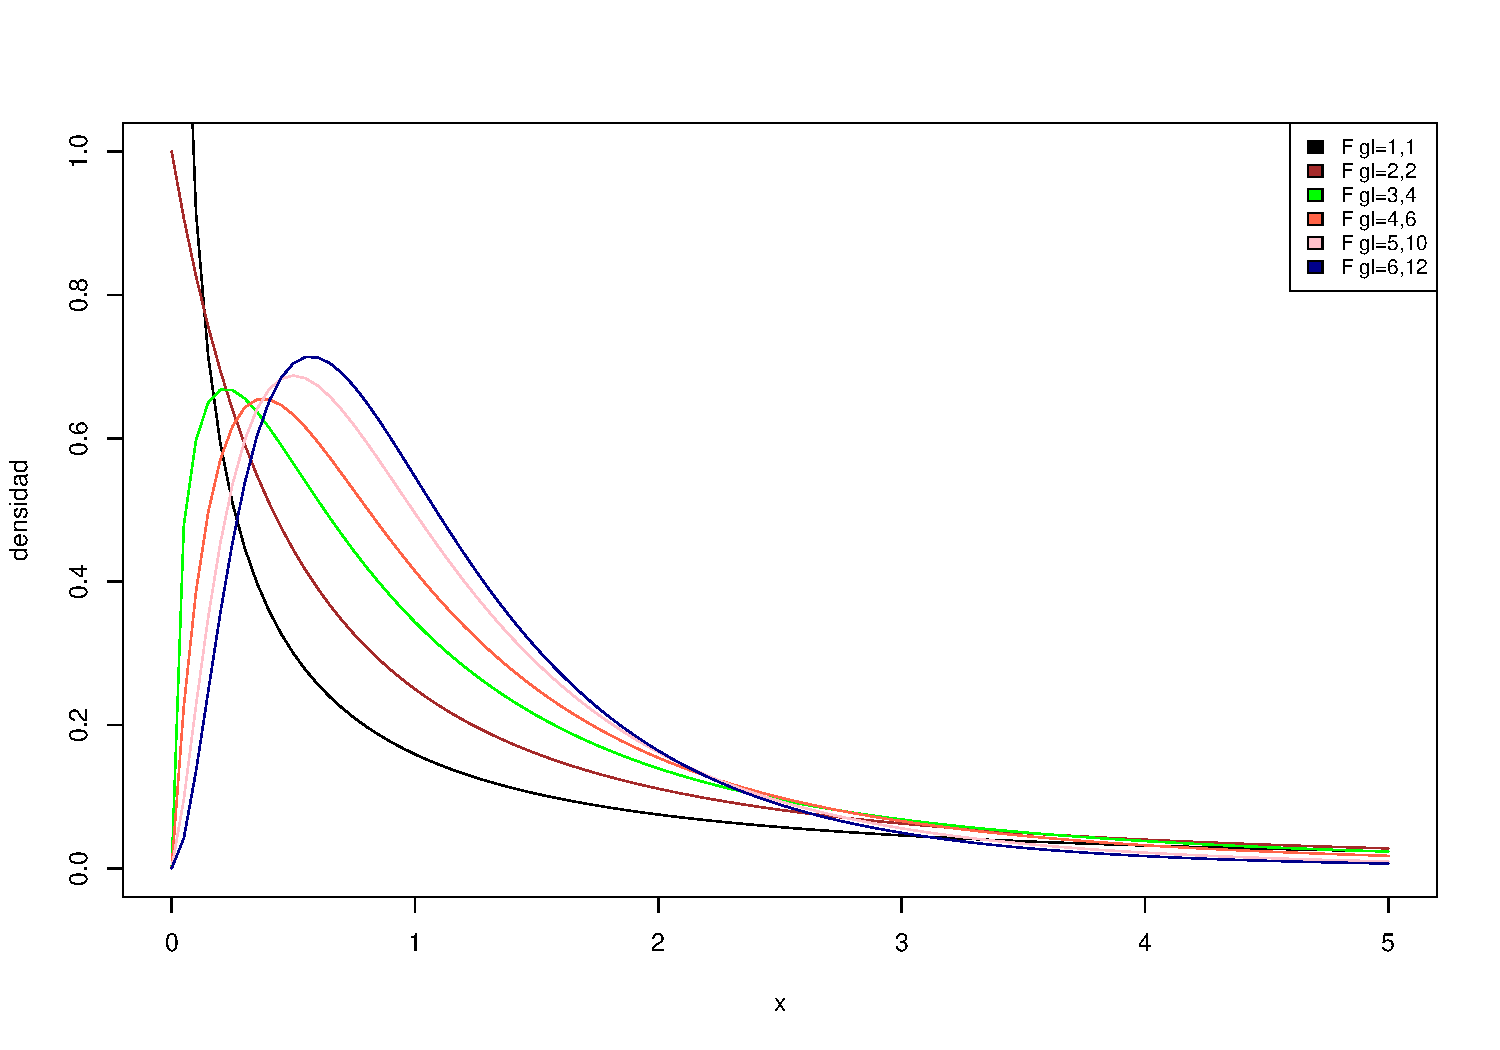
\includegraphics{contrastes_dos_muestras_files/figure-beamer/unnamed-chunk-53-1.pdf}
\end{frame}

\begin{frame}{p-valores}
\protect\hypertarget{p-valores}{}
Los \textbf{\(p\)-valores} asociados a los contrastes anteriores son:

\(p\)-valor: \(P(F_{n_1-1,n_2-1}\geq f_0)\).

\(p\)-valor: \(P(F_{n_1-1,n_2-1}\leq f_0)\).

\(p\)-valor:
\(\min\{2\cdot P(F_{n_1-1,n_2-1}\leq f_0),2\cdot P(F_{n_1-1,n_2-1}\geq f_0)\}\).
\end{frame}

\begin{frame}{Ejemplo}
\protect\hypertarget{ejemplo-48}{}
\textbf{Ejercicio}

Consideramos el ejemplo donde queríamos comparar los tiempos de
realización de una tarea entre estudiantes de dos grados \(G_1\) y
\(G_2\). Suponemos que estos tiempos siguen distribuciones normales.

Disponemos de dos muestras independientes de los tiempos usados por los
estudiantes de cada grado para realizar la tarea. Los tamaños de cada
muestra son \(n_1=n_2=40\).

Las desviaciones típicas muestrales de los tiempos empleados para cada
muestra son: \[
\widetilde{S}_1=1.201,\quad \widetilde{S}_2=1.579
\]

Contrastar la hipótesis de igualdad de varianzas al nivel de
significación \(0.05\).
\end{frame}

\begin{frame}{Ejemplo}
\protect\hypertarget{ejemplo-49}{}
El contraste planteado es el siguiente: \[
\left\{\begin{array}{l}
H_0:\sigma_1=\sigma_2,\\
H_1:\sigma_1\neq \sigma_2,
\end{array}\right.
\] donde \(\sigma_1\) y \(\sigma_2\) son las desviaciones típicas de los
tiempos empleados para realizar la tarea por los estudiantes de los
grados \(G_1\) y \(G_2\), respectivamente.

El \textbf{estadístico de contraste} para el contraste anterior es:
\(F=\frac{\widetilde{S}_1^2}{\widetilde{S}_2^2}\sim F_{39,39}\).

Dicho estadístico toma el siguiente valor:
\(f_0=\frac{1.201^2}{1.579^2}=0.579.\)
\end{frame}

\begin{frame}{Ejemplo}
\protect\hypertarget{ejemplo-50}{}
El \textbf{\(p\)-valor} para el contraste anterior será: \[
\begin{array}{l}
\min\{2\cdot P(F_{n_1-1,n_2-1}\leq f_0),2\cdot P(F_{n_1-1,n_2-1}\geq f_0)\}= \\
\min\{2\cdot P(F_{n_1-1,n_2-1}\leq 0.579),2\cdot P(F_{n_1-1,n_2-1}\geq 0.579)\} 
= \\ \min\{0.091,1.909\}=0.091.
\end{array}
\]

Decisión: como que el \(p\)-valor es moderado pero mayor que
\(\alpha=0.05\), no podemos rechazar la hipótesis que las dos varianzas
sean iguales.

Concluimos que no tenemos evidencias suficientes para rechazar que
\(\sigma_1= \sigma_2\).

Por tanto, en el contraste de las dos medias, tendríamos que suponer que
las varianzas de las dos poblaciones son la misma.
\end{frame}

\begin{frame}{Ejemplo}
\protect\hypertarget{ejemplo-51}{}
El \textbf{intervalo de confianza} para
\(\frac{\sigma_1^2}{\sigma_2^2}\) al nivel de confianza
\((1-\alpha)\cdot 100\%\) es \[
\left(\frac{\widetilde{S}_1^2}{\widetilde{S}_2^2}\cdot F_{n_1-1,n_2-1,\frac{\alpha}2},\frac{\widetilde{S}_1^2}{\widetilde{S}_2^2}\cdot F_{n_1-1,n_2-1,1-\frac{\alpha}2}\right) =
\left(\frac{1.201^2}{1.579^2}\cdot F_{39,39,0.025},\frac{1.201^2}{1.579^2}\cdot F_{39,39,0.975}\right)=(0.306,1.094)
\] Observemos que el intervalo de confianza anterior contiene el valor
1, hecho que reafirma la decisión tomada de no rechazar la hipótesis de
igualdad de varianzas.
\end{frame}

\begin{frame}{Ejemplo}
\protect\hypertarget{ejemplo-52}{}
\textbf{Ejemplo} Se desea comparar la actividad motora espontánea de un
grupo de 25 ratas control y otro de 36 ratas desnutridas. Se midió el
número de veces que pasaban ante una célula fotoeléctrica durante 24
horas. Los datos obtenidos fueron los siguientes:

\begin{longtable}[]{@{}llll@{}}
\toprule
& \(n\) & \(\overline{X}\) & \(\widetilde{S}\)\tabularnewline
\midrule
\endhead
1. Control & 25 & \(869.8\) & \(106.7\)\tabularnewline
2. Desnutridas & 36 & \(665\) & \(133.7\)\tabularnewline
\bottomrule
\end{longtable}

¿Se observan diferencias significativas entre el grupo de control y el
grupo desnutrido?

Supondremos que los datos anteriores provienen de poblaciones normales.
\end{frame}

\begin{frame}{Ejemplo}
\protect\hypertarget{ejemplo-53}{}
El contraste a realizar es el siguiente: \[
\left\{\begin{array}{l}
H_0:\mu_1=\mu_2,\\
H_1:\mu_1\neq \mu_2,
\end{array}\right.
\] donde \(\mu_1\) y \(\mu_2\) representan los valores medios del número
de veces que las ratas de control y desnutridas pasan ante la célula
fotoeléctrica, respectivamente.

Antes de nada, tenemos que averiguar si las varianzas de los dos grupos
son iguales o no ya que es un parámetro a usar en el contraste a
realizar.

Por tanto, en primer lugar, realizaremos el contraste: \[
\left\{\begin{array}{l}
H_0:\sigma_1=\sigma_2\\
H_1:\sigma_1\neq \sigma_2
\end{array}\right.
\] donde \(\sigma_1\) y \(\sigma_2\) representan las desviaciones
típicas del número de veces que las ratas de control y desnutridas pasan
ante la célula fotoeléctrica, respectivamente.
\end{frame}

\begin{frame}{Ejemplo}
\protect\hypertarget{ejemplo-54}{}
El \textbf{Estadístico de contraste} para el contraste anterior vale:
\(F=\frac{\widetilde{S}_1^2}{\widetilde{S}_2^2}\sim F_{24,35}.\)

El valor que toma es el siguiente:
\(f_0=\frac{106.7^2}{133.7^2}=0.637.\)

El \textbf{\(p\)-valor} para el contraste anterior vale: \[
\begin{array}{l}
\min\{2\cdot P(F_{n_1-1,n_2-1}\leq f_0),2\cdot P(F_{n_1-1,n_2-1}\geq f_0)\}= \\
\min\{2\cdot P(F_{n_1-1,n_2-1}\leq 0.637),2\cdot P(F_{n_1-1,n_2-1}\geq 0.637)\} 
= \\ \min\{0.251,1.749\}=0.251.
\end{array}
\] El \textbf{\(p\)-valor} es un valor grande, por tanto, concluimos que
no podemos rechazar la hipótesis nula y decidimos que las varianzas de
las dos poblaciones son iguales.
\end{frame}

\begin{frame}{Ejemplo}
\protect\hypertarget{ejemplo-55}{}
Realicemos a continuación el contraste pedido: \[
\left\{\begin{array}{l}
H_0:\mu_1=\mu_2\\
H_1:\mu_1\neq \mu_2
\end{array}\right.
\]

El \textbf{estadístico de contraste} al suponer que
\(\sigma_1= \sigma_2\), será:
\(T=\frac{\overline{X}_1-\overline{X}_2} {\sqrt{(\frac1{n_1}+\frac1{n_2})\cdot \frac{(n_1-1)\widetilde{S}_1^2+(n_2-1)\widetilde{S}_2^2} {n_1+n_2-2}}}\sim t_{59}\).

El valor que toma dicho estadístico en los valores muestrales vale:
\(t_0=\frac{869.8-665}{\sqrt{(\frac1{25}+\frac1{36})\cdot \frac{24\cdot 106.7^2+35\cdot 133.7^2} {25+36-2}}}=6.373.\)

El \textbf{\(p\)-valor} del contraste será:
\(p=2\cdot P(t_{59}\geq 6.373)\approx 0.\)

Decisión: como el \textbf{\(p\)-valor} es prácticamente nulo, concluimos
que tenemos evidencias suficientes para rechazar la hipótesis nula y por
tanto hay diferencias entre las ratas de control y las desnutridas entre
el número de veces que pasan ante la célula fotoeléctrica.
\end{frame}

\begin{frame}[fragile]{Contrastes para varianzas en \texttt{R}}
\protect\hypertarget{contrastes-para-varianzas-en-r}{}
La función para efectuar este test en \texttt{R} es \texttt{var.test}y
su sintaxis básica es la misma que la de \texttt{t.test} para dos
muestras:

\begin{Shaded}
\begin{Highlighting}[]
\KeywordTok{var.test}\NormalTok{(x, y, }\DataTypeTok{alternative=}\NormalTok{..., }\DataTypeTok{conf.level=}\NormalTok{...)}
\end{Highlighting}
\end{Shaded}

donde \texttt{x} e \texttt{y} son los dos vectores de datos, que se
pueden especificar mediante una fórmula como en el caso de
\texttt{t.test}, y el parámetro \texttt{alternative} puede tomar los
tres mismos valores que en los tests anteriores.
\end{frame}

\begin{frame}[fragile]{Contrastes para varianzas en \texttt{R}. Ejemplo}
\protect\hypertarget{contrastes-para-varianzas-en-r.-ejemplo}{}
\textbf{Ejercicio}

Recordemos que cuando explicábamos el contraste para dos medias
independientes, contrastamos si las medias de las longitudes del pétalo
para las especies setosa y versicolor eran iguales o no pero
necesitábamos saber si las varianzas eran iguales o no para poder
tenerlo en cuenta en la función \texttt{t.test}.

Veamos ahora si podemos considerar las varianzas iguales o no.

Las muestras eran \texttt{muestra.setosa} y \texttt{muestra.versicolor}.
\end{frame}

\begin{frame}[fragile]{Contrastes para varianzas en \texttt{R}. Ejemplo}
\protect\hypertarget{contrastes-para-varianzas-en-r.-ejemplo-1}{}
Realicemos el contraste de igualdad de varianzas:

\begin{Shaded}
\begin{Highlighting}[]
\KeywordTok{var.test}\NormalTok{(muestra.setosa}\OperatorTok{$}\NormalTok{Petal.Length,muestra.versicolor}\OperatorTok{$}\NormalTok{Petal.Length)}
\end{Highlighting}
\end{Shaded}

\begin{verbatim}
## 
##  F test to compare two variances
## 
## data:  muestra.setosa$Petal.Length and muestra.versicolor$Petal.Length
## F = 0.14, num df = 39, denom df = 39, p-value = 0.00000002
## alternative hypothesis: true ratio of variances is not equal to 1
## 95 percent confidence interval:
##  0.0758 0.2710
## sample estimates:
## ratio of variances 
##             0.1433
\end{verbatim}
\end{frame}

\begin{frame}[fragile]{Contrastes para varianzas en \texttt{R}. Ejemplo}
\protect\hypertarget{contrastes-para-varianzas-en-r.-ejemplo-2}{}
El p-valor del contraste ha sido prácticamente cero. Por tanto,
concluimos que tenemos evidencias suficientes para afirmar que las
varianzas de las longitudes del pétalo de las flores de las especies
setosa y versicolor son diferentes.

Si nos fijamos en el intervalo de confianza en el cociente de varianzas
\(\frac{\sigma^2_{{ setosa}}}{\sigma^2_{{versicolor}}}\),

\begin{Shaded}
\begin{Highlighting}[]
\KeywordTok{var.test}\NormalTok{(muestra.setosa}\OperatorTok{$}\NormalTok{Petal.Length,muestra.versicolor}\OperatorTok{$}\NormalTok{Petal.Length)}\OperatorTok{$}\NormalTok{conf.int}
\end{Highlighting}
\end{Shaded}

\begin{verbatim}
## [1] 0.0758 0.2710
## attr(,"conf.level")
## [1] 0.95
\end{verbatim}

vemos que no contiene el valor 1, de hecho está a la izquierda de él.
Este hecho nos hace reafirmar la conclusión anterior.

Para que el contraste anterior tenga sentido, hemos de suponer que las
longitudes del pétalo de las flores de las especies setosa y versicolor
siguen distribuciones normales.
\end{frame}

\begin{frame}[fragile]{Contrastes para varianzas}
\protect\hypertarget{contrastes-para-varianzas}{}
\begin{itemize}[<+->]
\item
  Hemos insistido en que el test F solo es válido si las dos poblaciones
  cuyas varianzas comparamos son normales.
\item
  ¿Qué podemos hacer si dudamos de su normalidad? Usar un test no
  paramétrico que no presuponga esta hipótesis.
\item
  Hay diversos tests no paramétricos para realizar contrastes
  bilaterales de dos varianzas. Aquí os recomendamos el \textbf{test de
  Fligner-Killeen}, implementado en la función \texttt{fligner.test}.

  \begin{itemize}[<+->]
  \tightlist
  \item
    Se aplica o bien a una \texttt{list} formada por las dos muestras, o
    bien a una fórmula que separe un vector numérico en dos muestras por
    medio de un factor de dos niveles.
  \end{itemize}
\end{itemize}
\end{frame}

\begin{frame}[fragile]{Contrastes para varianzas. Ejemplo.}
\protect\hypertarget{contrastes-para-varianzas.-ejemplo.}{}
Realicemos el contraste previo de igualdad de varianzas usando el test
no paramétrico anterior para ver si llegamos a la misma conclusión:

\begin{Shaded}
\begin{Highlighting}[]
\KeywordTok{fligner.test}\NormalTok{(}\KeywordTok{list}\NormalTok{(muestra.setosa}\OperatorTok{$}\NormalTok{Petal.Length,muestra.versicolor}\OperatorTok{$}\NormalTok{Petal.Length))}
\end{Highlighting}
\end{Shaded}

\begin{verbatim}
## 
##  Fligner-Killeen test of homogeneity of variances
## 
## data:  list(muestra.setosa$Petal.Length, muestra.versicolor$Petal.Length)
## Fligner-Killeen:med chi-squared = 22, df = 1, p-value = 0.000002
\end{verbatim}

Como el p-valor vuelve a ser insignificante, llegamos a la misma
conclusión anterior: tenemos evidencias suficientes para afirmar que las
varianzas de las longitudes del pétalo de las flores de las especies
setosa y versicolor son diferentes.

La ventaja de este test es que no necesitamos la normalidad de las
muestras, aunque su potencia, que explicaremos más adelante, sea
inferior.
\end{frame}

\hypertarget{muestras-emparejadas}{%
\section{Muestras emparejadas}\label{muestras-emparejadas}}

\begin{frame}{Introducción}
\protect\hypertarget{introducciuxf3n-5}{}
Las muestras consideradas hasta el momento se han supuesto
\textbf{independientes}.

Un caso completamente diferente es cuando las dos muestras corresponden
a los mismos individuos o a individuos emparejados por algún factor.

Ejemplos:

\begin{itemize}[<+->]
\item
  Se estudia el estado de una dolencia a los mismos individuos antes y
  después de un tratamiento.
\item
  Se mide la incidencia de cáncer en parejas de hermanos gemelos.
\end{itemize}

En estos casos, se habla de \textbf{muestras emparejadas}, o
\textbf{paired samples} en inglés.
\end{frame}

\begin{frame}{Introducción}
\protect\hypertarget{introducciuxf3n-6}{}
Para decidir si hay diferencias entre los valores de dos
\textbf{muestras emparejadas}, el contraste más común consiste a
calcular las diferencias de los valores de cada una de las parejas de
muestras y realizar un contraste para averiguar si la media de las
diferencias es 0.

Observación: El \textbf{diseño experimental} para realizar un contraste
de \textbf{muestras emparejadas} se tiene que fijar \textbf{antes} de la
\textbf{recogida de datos}.
\end{frame}

\begin{frame}{Contrastes de medias de muestras emparejadas}
\protect\hypertarget{contrastes-de-medias-de-muestras-emparejadas}{}
En el caso de un contraste de muestras emparejadas, sean \(X_1\) y
\(X_2\) las variables correspondientes y sean \[
\begin{array}{l}
X_{1,1}, X_{1,2},\ldots, X_{1,n},\mbox{ de }X_1\\
X_{2,1}, X_{2,2},\ldots, X_{2,n},\mbox{ de }X_2
\end{array}
\] las m.a.s. de cada una de las variables correspondientes a las dos
muestras.

Fijémonos que, al ser la muestras emparejadas, los tamaños de las mismas
deben ser iguales.

Consideramos la variable diferencia \(D=X_1-X_2\). La m.a.s. de \(D\)
construida a partir de las muestras anteriores será: \[
D_1 =X_{1,1}-X_{2,1}, \ D_2=X_{1,2}-X_{2,2},\ldots, D_n=X_{1,n}-X_{2,n}.
\]
\end{frame}

\begin{frame}{Contrastes de medias de muestras emparejadas}
\protect\hypertarget{contrastes-de-medias-de-muestras-emparejadas-1}{}
Los contastes planteados son los siguientes:

\(\left\{\begin{array}{l} H_0:\mu_1=\mu_2,\\ H_1:\mu_1> \mu_2. \end{array}\right.\)

\(\left\{\begin{array}{l} H_0:\mu_1=\mu_2,\\ H_1:\mu_1< \mu_2. \end{array}\right.\)

\(\left\{\begin{array}{l} H_0:\mu_1=\mu_2,\\ H_1:\mu_1\neq \mu_2. \end{array}\right.\)
\end{frame}

\begin{frame}{Contrastes de medias de muestras emparejadas}
\protect\hypertarget{contrastes-de-medias-de-muestras-emparejadas-2}{}
que, escritos en términos de la media de la variable diferencia \(D\),
\(\mu_d\), serán:

\(\left\{\begin{array}{l} H_0:\mu_d=0,\\ H_1:\mu_d> 0. \end{array}\right.\)

\(\left\{\begin{array}{l} H_0:\mu_d=0,\\ H_1:\mu_d< 0. \end{array}\right.\)

\(\left\{\begin{array}{l} H_0:\mu_d=0,\\ H_1:\mu_d\neq 0. \end{array}\right.\)
\end{frame}

\begin{frame}{Contrastes de medias de muestras emparejadas}
\protect\hypertarget{contrastes-de-medias-de-muestras-emparejadas-3}{}
O sea, hemos reducido un contraste de medias de dos muestras
dependientes a un contraste de una sola media de una sola muestra.

A partir de aquí, podemos calcular los \textbf{p-valores} y los
\textbf{intervalos de confianza} de los contrates anteriores usando las
expresiones de los contrastes de una media de una sola media vistos
anteriormente.
\end{frame}

\begin{frame}{Ejemplo de medias emparejadas}
\protect\hypertarget{ejemplo-de-medias-emparejadas}{}
\textbf{Ejemplo de medias emparejadas}

Disponemos de dos algoritmos de alineamiento de proteínas. Los dos
producen resultados de la misma calidad.

Estamos interesados en saber cuál de los dos algoritmos es \emph{más
eficiente}, en el sentido de tener un tiempo de ejecución más corto.
Suponemos que dichos tiempos de ejecución siguen leyes normales.

Tomamos una muestra de proteínas y les aplicamos los dos algoritmos,
anotando los tiempos de ejecución sobre cada proteína.

Los resultados obtenidos son:

\begin{longtable}[]{@{}lllllllllll@{}}
\toprule
& 1 & 2 & 3 & 4 & 5 & 6 & 7 & 8 & 9 & 10\tabularnewline
\midrule
\endhead
algoritmo 1 & 8.1 & 11.9 & 11.4 & 12.9 & 9.0 & 7.2 & 12.4 & 6.9 & 8.9 &
8.3\tabularnewline
algoritmo 2 & 6.9 & 6.7 & 8.3 & 8.6 & 18.9 & 7.9 & 7.4 & 8.7 & 7.9 &
12.4\tabularnewline
diferencias & 1.2 & 5.2 & 3.1 & 4.3 & -9.9 & -0.7 & 5.0 & -1.8 & 1.0 &
-4.1\tabularnewline
\bottomrule
\end{longtable}
\end{frame}

\begin{frame}{Ejemplo de medias emparejadas}
\protect\hypertarget{ejemplo-de-medias-emparejadas-1}{}
La media y la desviación típica muestrales de las difencias son
\(\overline{d}=0.33,\) \(\tilde s_d = 4.715.\)

Queremos contrastar la igualdad de medias con el test que corresponda. Y
si son diferentes, decidir cuál tiene mayor tiempo de ejecución.

O sea, queremos realizar el contraste siguiente: \[
\left\{\begin{array}{l}
H_0:\mu_1=\mu_2,\\
H_1:\mu_1\neq \mu_2,
\end{array}\right.
\] donde \(\mu_1\) y \(\mu_2\) son los tiempos de ejecución de los
algoritmos 1 y 2, respectivamente.

Escribimos el contraste anterior en función de \(\mu_d\), la media de
las diferencias de los tiempos de ejecución entre los dos algoritmos: \[
\left\{\begin{array}{l}
H_0:\mu_d=0,\\
H_1:\mu_d\neq 0.
\end{array}\right.
\]
\end{frame}

\begin{frame}{Ejemplo de medias emparejadas}
\protect\hypertarget{ejemplo-de-medias-emparejadas-2}{}
El \textbf{estadístico de contraste} para el contraste anterior es
\(T=\frac{\overline{d}}{\widetilde{S}_d/\sqrt{n}},\) que tiene
distribución \(t_{n-1}=t_{9}\).

Dicho estadístico toma el siguiente valor usando los valores muestrales:
\(t_0=\frac{0.33}{4.715/\sqrt{10}}=0.221.\)

El \textbf{\(p\)-valor} del contraste anterior será:
\(p=2\cdot p(t_{9} > |0.221|) =0.83.\)

Es un valor grande. Por tanto, no tenemos evidencias suficientes para
rechazar la hipótesis nula y concluimos que los tiempos de ejecución de
los dos algoritmos es el mismo.
\end{frame}

\begin{frame}[fragile]{Contrastes para medias emparejadas en \texttt{R}.
El test t}
\protect\hypertarget{contrastes-para-medias-emparejadas-en-r.-el-test-t}{}
Recordemos la sintaxis básica del test t en \texttt{R}

\begin{Shaded}
\begin{Highlighting}[]
\KeywordTok{t.test}\NormalTok{(x, y, }\DataTypeTok{mu=}\NormalTok{..., }\DataTypeTok{alternative=}\NormalTok{..., }\DataTypeTok{conf.level=}\NormalTok{..., }\DataTypeTok{paired=}\NormalTok{..., }
       \DataTypeTok{var.equal=}\NormalTok{..., }\DataTypeTok{na.omit=}\NormalTok{...)}
\end{Highlighting}
\end{Shaded}

donde el único parámetro para indicarle si las muestras son emparejadas
o independientes es el parámetro \texttt{paired}: con
\texttt{paired=TRUE} indicamos que las muestras son emparejadas, y con
\texttt{paired=FALSE} (que es su valor por defecto) que son
independientes.
\end{frame}

\begin{frame}[fragile]{Ejemplo de dos muestras dependientes con
\texttt{R}}
\protect\hypertarget{ejemplo-de-dos-muestras-dependientes-con-r}{}
\textbf{Ejercicio}

Nos planteamos si la longitud del sépalo supera la longitud del pétalo
para las flores de la especie virginica en la tabla de datos
\texttt{iris}.

En este caso se trataría de un contraste de medias dependientes: \[
\left.
\begin{array}{ll}
H_0: & \mu_{{sépalo,virginica}} =\mu_{{pétalo,virginica}}, \\
H_1: & \mu_{{sépalo,virginica}} > \mu_{{pétalo,virginica}},
\end{array}
\right\}
\] donde \(\mu_{{sépalo,virginica}}\) y \(\mu_{{pétalo,virginica}}\) son
las longitudes del sépalo y del pétalo de las flores de la especie
virginica.
\end{frame}

\begin{frame}[fragile]{Ejemplo de dos muestras dependientes con
\texttt{R}}
\protect\hypertarget{ejemplo-de-dos-muestras-dependientes-con-r-1}{}
Para realizar dicho contraste, vamos a considerar una muestra de 40
flores de la especie virgínica y sobre \textbf{las mismas flores}
calcular las longitudes del sépalo y del pétalo.

En primer lugar seleccionamos las flores de la muestra:

\begin{Shaded}
\begin{Highlighting}[]
\KeywordTok{set.seed}\NormalTok{(}\DecValTok{100}\NormalTok{)}
\NormalTok{flores.elegidas.virginica=}\KeywordTok{sample}\NormalTok{(}\DecValTok{101}\OperatorTok{:}\DecValTok{150}\NormalTok{,}\DecValTok{40}\NormalTok{,}\DataTypeTok{replace=}\OtherTok{TRUE}\NormalTok{)}
\end{Highlighting}
\end{Shaded}

La muestra elegida será:

\begin{Shaded}
\begin{Highlighting}[]
\NormalTok{muestra.virginica =}\StringTok{ }\NormalTok{iris[flores.elegidas.virginica,]}
\end{Highlighting}
\end{Shaded}
\end{frame}

\begin{frame}[fragile]{Ejemplo de dos muestras dependientes con
\texttt{R}}
\protect\hypertarget{ejemplo-de-dos-muestras-dependientes-con-r-2}{}
El contraste a realizar es el siguiente:

\begin{Shaded}
\begin{Highlighting}[]
\KeywordTok{t.test}\NormalTok{(muestra.virginica}\OperatorTok{$}\NormalTok{Sepal.Length,muestra.virginica}\OperatorTok{$}\NormalTok{Petal.Length,}
       \DataTypeTok{paired=}\OtherTok{TRUE}\NormalTok{,}\DataTypeTok{alternative=}\StringTok{"greater"}\NormalTok{)}
\end{Highlighting}
\end{Shaded}

\begin{verbatim}
## 
##  Paired t-test
## 
## data:  muestra.virginica$Sepal.Length and muestra.virginica$Petal.Length
## t = 22, df = 39, p-value <0.0000000000000002
## alternative hypothesis: true difference in means is greater than 0
## 95 percent confidence interval:
##  0.9051    Inf
## sample estimates:
## mean of the differences 
##                    0.98
\end{verbatim}
\end{frame}

\begin{frame}{Ejemplo de dos muestras dependientes con \texttt{R}}
\protect\hypertarget{ejemplo-de-dos-muestras-dependientes-con-r-3}{}
Vemos que el p-valor del contraste es prácticamente nulo, lo que nos
hace concluir que tenemos evidencias suficientes para afirmar que la
longitud del sépalo es superior a la longitud del pétalo para las flores
de la especie virginica.

Fijémonos que la media de la diferencia entre las medias de las
longitudes del sépalo y del pétalo vale 0.98, valor suficientemente
alejado del cero para poder afirmar que la media de la longitud del
sépalo es superior a la media de la longitud del pétalo.
\end{frame}

\begin{frame}[fragile]{Ejemplo de dos muestras dependientes con
\texttt{R}}
\protect\hypertarget{ejemplo-de-dos-muestras-dependientes-con-r-4}{}
El intervalo de confianza al 95\% de confianza para la diferencia de
medias asociado al contraste anterior vale:

\begin{Shaded}
\begin{Highlighting}[]
\KeywordTok{t.test}\NormalTok{(muestra.virginica}\OperatorTok{$}\NormalTok{Sepal.Length,muestra.virginica}\OperatorTok{$}\NormalTok{Petal.Length,}
       \DataTypeTok{paired=}\OtherTok{TRUE}\NormalTok{,}\DataTypeTok{alternative=}\StringTok{"greater"}\NormalTok{)}\OperatorTok{$}\NormalTok{conf.int}
\end{Highlighting}
\end{Shaded}

\begin{verbatim}
## [1] 0.9051    Inf
## attr(,"conf.level")
## [1] 0.95
\end{verbatim}

intervalo que no contiene el cero y que está a la derecha del mismo, lo
que nos hace reafirmar que tenemos evidencias suficientes para rechazar
la hipótesis nula \(H_0\).
\end{frame}

\begin{frame}{Contrastes de proporciones de muestras emparejadas}
\protect\hypertarget{contrastes-de-proporciones-de-muestras-emparejadas}{}
Supongamos que evaluamos dos características dicotómicas sobre una misma
muestra de \(n\) sujetos. Resumimos los resultados obtenidos en la tabla
siguiente:

\[
\begin{array}{r|c}
 & \ \mbox{Característica 1}\  \\
\mbox{Característica 2} &\ \ \, \mbox{Sí}\qquad \mbox{No}\\\hline
 \mbox{Sí} & \quad\ \  a \qquad \ \ \, b\quad  \\
 \mbox{No} & \quad\ \   c  \qquad \ \ \, d\quad
 \end{array}
\]
\end{frame}

\begin{frame}[fragile]{Contrastes para proporciones. Muestras
emparejadas}
\protect\hypertarget{contrastes-para-proporciones.-muestras-emparejadas}{}
Se cumple \(a+b+c+d=n\). Esta tabla quiere decir, naturalmente, que
\(a\) sujetos de la muestra tuvieron la característica 1 y la
característica 2, que \(b\) sujetos de la muestra tuvieron la
característica 2 y pero no tuvieron la característica 2, etc.

Vamos a llamar \(p_{1}\) a la proporción poblacional de individuos con
la característica 1, y \(p_{2}\) a la proporción poblacional de
individuos con la característica 2.

Queremos contrastar la hipótesis nula \(H_{0}:p_1=p_2\) contra alguna
hipótesis alternativa. En este caso, no pueden usarse las funciones
\texttt{prop.test} o \texttt{fisher.test}.
\end{frame}

\begin{frame}{Contrastes para proporciones. Muestras emparejadas}
\protect\hypertarget{contrastes-para-proporciones.-muestras-emparejadas-1}{}
La solución es realizar el contraste bilateral: (o los unilaterales
asociados) \[
\left\{\begin{array}{l}
H_{0}:p_1=p_2,\\
H_{1}:p_1\neq p_2.
\end{array}\right.
\] Dicho contraste tiene sentido cuando \(n\) es grande y el número
\(b+c\) de \textbf{casos discordantes} (en los que una característica da
Sí y la otra da No) es razonablemente grande, pongamos \(\geq 20\).
\end{frame}

\begin{frame}{Contrastes para proporciones. Muestras emparejadas}
\protect\hypertarget{contrastes-para-proporciones.-muestras-emparejadas-2}{}
El \textbf{estadístico de contraste} para el contraste anterior es
\(Z=\frac{\frac{b}{n}-\frac{c}{n}}{\sqrt{\frac{b+c}{n^2}}}\), cuya
distribución aproximada es una \(N(0,1)\). Sea \(z_0\) el valor que toma
sobre los valores muestrales.

Por tanto el \textbf{\(p\)-valor} será: \(p=2\cdot p(Z > |z_0|)\).

\textbf{Ejercicio}

Hallar los \textbf{\(p\)-valores} para los contrastes unilaterales.
\end{frame}

\begin{frame}{Ejemplo de proporciones emparejadas}
\protect\hypertarget{ejemplo-de-proporciones-emparejadas}{}
\textbf{Ejemplo de proporciones emparejadas}

Se toma una muestra de \(1000\) personas afectadas por migraña. Se les
facilita un fármaco porque aligere los síntomas.

Después de la administración se les pregunta si han notado alivio en el
dolor.

Al cabo de un tiempo se suministra a los mismos individuos un placebo y
se les vuelve a preguntar si han notado o no mejora.

Nos preguntamos si es más efectivo el fármaco que el placebo en base a
los resultados del estudio:

\begin{longtable}[]{@{}lll@{}}
\toprule
Fármaco/Placebo & Si & No\tabularnewline
\midrule
\endhead
Si & 300 & 62\tabularnewline
No & 38 & 600\tabularnewline
\bottomrule
\end{longtable}
\end{frame}

\begin{frame}{Ejemplo de proporciones emparejadas}
\protect\hypertarget{ejemplo-de-proporciones-emparejadas-1}{}
El contraste que nos piden realizar es el siguiente: \[
\left\{\begin{array}{l}
H_0:p_1=p_2\\
H_1:p_1> p_2
\end{array}\right.
\] donde \(p_1\) y \(p_2\) representan las proporciones de gente que
encuentra mejora con el fármaco y el placebo, respectivamente.

El estadístico de contraste para el contraste anterior es:
\(Z=\frac{\frac{b}{n}-\frac{c}{n}}{\sqrt{\frac{b+c}{n^2}}}\), cuya
distribución aproximada es una \(N(0,1)\), donde \(a=300\), \(b=62\),
\(c=38\) y \(d=600\) en nuestro caso.

El valor que toma dicho estadístico es:
\(z_0 = \frac{\frac{62}{1000}-\frac{38}{1000}}{\sqrt{\frac{62+38}{1000^2}}} =2.4.\)
\end{frame}

\begin{frame}{Ejemplo de proporciones emparejadas}
\protect\hypertarget{ejemplo-de-proporciones-emparejadas-2}{}
Este contraste solo es válido cuando la muestra es grande y el número de
\emph{casos discordantes} \(b+d\) (100 en nuestro caso) es ``bastante
grande'', \(\geq 20\).

El \textbf{\(p\)-valor} para el contraste considerado es
\(P(Z>2.4)=0.008,\) pequeño.

Por lo tanto, concluimos que tenemos evidencias suficientes para
rechazar la hipótesis nula y poder afirmar que el fármaco es más
efectivo que el placebo.
\end{frame}

\begin{frame}[fragile]{Contrastes para proporciones de muestras
emparejadas en \texttt{R}}
\protect\hypertarget{contrastes-para-proporciones-de-muestras-emparejadas-en-r}{}
En \texttt{R} podemos usar el \textbf{test de McNemar}, que se lleva a
cabo con la instrucción \texttt{mcnemar.test}. Su sintaxis básica es

\begin{Shaded}
\begin{Highlighting}[]
\KeywordTok{mcnemar.test}\NormalTok{(X)}
\end{Highlighting}
\end{Shaded}

donde \texttt{X} es la matriz
\(\left(\begin{array}{cc} a & b\\ c& d \end{array}\right)\) que
corresponde a la tabla anterior.
\end{frame}

\begin{frame}[fragile]{Contrastes para proporciones de muestras
emparejadas en \texttt{R}. Ejemplo}
\protect\hypertarget{contrastes-para-proporciones-de-muestras-emparejadas-en-r.-ejemplo}{}
\textbf{Ejercicio}

Usando la tabla de datos \textbf{birthw} del paquete \textbf{MASS},
vamos a ver si la proporción de madres fumadoras es la misma que la
proporción de madres hipertensas.

Para ello, vamos a considerar una muestra de 30 madres y vamos a
realizar el contraste correspondiente.

En primer lugar elegimos las madres y consideramos la muestra
correspondiente:

\begin{Shaded}
\begin{Highlighting}[]
\KeywordTok{set.seed}\NormalTok{(}\DecValTok{333}\NormalTok{)}
\NormalTok{madres.elegidas.prop.empar =}\StringTok{ }\KeywordTok{sample}\NormalTok{(}\DecValTok{1}\OperatorTok{:}\DecValTok{189}\NormalTok{,}\DecValTok{30}\NormalTok{,}\DataTypeTok{replace=}\OtherTok{TRUE}\NormalTok{)}
\NormalTok{muestra.madres.prop.empar =}\StringTok{ }\NormalTok{birthwt[madres.elegidas.prop.empar,]}
\end{Highlighting}
\end{Shaded}
\end{frame}

\begin{frame}[fragile]{Contrastes para proporciones de muestras
emparejadas en \texttt{R}. Ejemplo}
\protect\hypertarget{contrastes-para-proporciones-de-muestras-emparejadas-en-r.-ejemplo-1}{}
Seguidamente, calculamos la matriz para usar en el contraste:

\begin{Shaded}
\begin{Highlighting}[]
\NormalTok{(}\DataTypeTok{matriz.prop.empar =} \KeywordTok{table}\NormalTok{(muestra.madres.prop.empar}\OperatorTok{$}\NormalTok{smoke,muestra.madres.prop.empar}\OperatorTok{$}\NormalTok{ht))}
\end{Highlighting}
\end{Shaded}

\begin{verbatim}
##    
##      0  1
##   0 16  3
##   1 10  1
\end{verbatim}

Fijémonos que dicha matriz no es correcta ya que \(a=1\), \(b=10\),
\(c=3\) y \(d=16\). Arreglamos la matriz:

\begin{Shaded}
\begin{Highlighting}[]
\NormalTok{matriz.prop.empar =}\StringTok{ }\KeywordTok{rbind}\NormalTok{(matriz.prop.empar[}\DecValTok{2}\NormalTok{,],matriz.prop.empar[}\DecValTok{1}\NormalTok{,])}
\NormalTok{matriz.prop.empar =}\StringTok{ }\KeywordTok{cbind}\NormalTok{(matriz.prop.empar[,}\DecValTok{2}\NormalTok{],matriz.prop.empar[,}\DecValTok{1}\NormalTok{])}
\end{Highlighting}
\end{Shaded}
\end{frame}

\begin{frame}[fragile]{Contrastes para proporciones de muestras
emparejadas en \texttt{R}. Ejemplo}
\protect\hypertarget{contrastes-para-proporciones-de-muestras-emparejadas-en-r.-ejemplo-2}{}
Comprobamos que es correcta:

\begin{Shaded}
\begin{Highlighting}[]
\NormalTok{matriz.prop.empar}
\end{Highlighting}
\end{Shaded}

\begin{verbatim}
##      [,1] [,2]
## [1,]    1   10
## [2,]    3   16
\end{verbatim}
\end{frame}

\begin{frame}[fragile]{Contrastes para proporciones de muestras
emparejadas en \texttt{R}. Ejemplo}
\protect\hypertarget{contrastes-para-proporciones-de-muestras-emparejadas-en-r.-ejemplo-3}{}
Por último, realizamos el contraste planteado:

\begin{Shaded}
\begin{Highlighting}[]
\KeywordTok{mcnemar.test}\NormalTok{(matriz.prop.empar)}
\end{Highlighting}
\end{Shaded}

\begin{verbatim}
## 
##  McNemar's Chi-squared test with continuity correction
## 
## data:  matriz.prop.empar
## McNemar's chi-squared = 2.8, df = 1, p-value = 0.1
\end{verbatim}
\end{frame}

\begin{frame}{Contrastes para proporciones de muestras emparejadas en
\texttt{R}. Ejemplo}
\protect\hypertarget{contrastes-para-proporciones-de-muestras-emparejadas-en-r.-ejemplo-4}{}
Hemos obtenido un p-valor de 0.0961, valor que está entre 0.05 y 0.1, la
llamada zona de penumbra donde no se puede tomar una decisión clara.

Podemos decir, si consideramos que el p-valor es suficientemente grande,
que no tenemos evidencias suficientes para aceptar que la proporción de
madres fumadoras y con hipertensión sea diferente.

En otras palabras, no rechazamos la hipótesis nula \(H_0\).

Ahora bien, hay que tener en cuenta que el p-valor no es demasiado
grande para tal conclusión.
\end{frame}

\begin{frame}[fragile]{Contrastes para proporciones. Muestras
emparejadas.}
\protect\hypertarget{contrastes-para-proporciones.-muestras-emparejadas.}{}
Otra posibilidad para realizar un contraste de dos proporciones usando
muestras emparejadas, que no requiere de ninguna hipótesis sobre los
tamaños de las muestras, es usar de manera adecuada la función
\texttt{binom.test}.

Para explicar este método, consideremos la tabla siguiente, donde ahora
damos las probabilidades poblacionales de las cuatro combinaciones de
resultados: \[
\begin{array}{r|c}
 & \ \mbox{Característica 1}\  \\
\mbox{Característica 2} &\quad \ \!\mbox{Sí}\qquad\quad\, \mbox{No}\quad \\\hline
 \mbox{Sí} & \quad \  p_{11}  \qquad\quad p_{01}\quad  \\
 \mbox{No} & \quad \  p_{10} \qquad\quad  p_{00}\quad
 \end{array}
\]
\end{frame}

\begin{frame}{Contrastes para proporciones. Muestras emparejadas.}
\protect\hypertarget{contrastes-para-proporciones.-muestras-emparejadas.-1}{}
De esta manera \(p_1=p_{11}+p_{10}\) y \(p_2=p_{11}+p_{01}\).

Entonces, \(p_1=p_2\) es equivalente a \(p_{10}=p_{01}\) y cualquier
hipótesis alternativa se traduce en la misma desigualdad, pero para
\(p_{10}\) y \(p_{01}\):

\begin{itemize}[<+->]
\item
  \(p_1\neq p_2\) es equivalente a \(p_{10}\neq p_{01}\);
\item
  \(p_1< p_2\) es equivalente a \(p_{10}< p_{01}\); y
\item
  \(p_1> p_2\) es equivalente a \(p_{10}> p_{01}\).
\end{itemize}

Por lo tanto podemos traducir el contraste sobre \(p_1\) y \(p_2\) al
mismo contraste sobre \(p_{10}\) y \(p_{01}\).
\end{frame}

\begin{frame}{Contrastes para proporciones. Muestras emparejadas.}
\protect\hypertarget{contrastes-para-proporciones.-muestras-emparejadas.-2}{}
La gracia ahora está en que si la hipótesis nula \(p_{10}=p_{01}\) es
cierta, entonces, en el total de casos discordantes, el número de
sujetos en los que la característica 1 da Sí y la característica 2 da No
sigue una ley binomial con \(p=0.5\).

Por lo tanto, podemos efectuar el contraste usando un test binomial
exacto tomando

\begin{itemize}[<+->]
\item
  como muestra los casos discordantes de nuestra muestra, de tamaño
  \(b+c\),
\item
  como éxitos los sujetos que han dado Sí en la característica 1 y No en
  la característica 2, de tamaño \(c\),
\item
  con proporción a contrastar \(p=0.5\) y con hipótesis alternativa la
  que corresponda.
\end{itemize}
\end{frame}

\begin{frame}{Contrastes para proporciones. Muestras emparejadas.}
\protect\hypertarget{contrastes-para-proporciones.-muestras-emparejadas.-3}{}
La ventaja de este test es que su validez no requiere de ninguna
hipótesis sobre los tamaños de las muestras. El inconveniente es que el
intervalo de confianza que nos dará será para
\(p_{10}/(p_{10}+p_{01})\), y no permite obtener un intervalo de
confianza para la diferencia o el cociente de las probabilidades \(p_1\)
y \(p_2\) de interés.
\end{frame}

\begin{frame}[fragile]{Contrastes para proporciones de muestras
emparejadas en \texttt{R}. Ejemplo}
\protect\hypertarget{contrastes-para-proporciones-de-muestras-emparejadas-en-r.-ejemplo-5}{}
\textbf{Ejercicio}

Volvamos a realizar el contraste anterior usando este método.

Recordemos que la matriz de proporciones era:

\begin{Shaded}
\begin{Highlighting}[]
\NormalTok{matriz.prop.empar}
\end{Highlighting}
\end{Shaded}

\begin{verbatim}
##      [,1] [,2]
## [1,]    1   10
## [2,]    3   16
\end{verbatim}
\end{frame}

\begin{frame}[fragile]{Contrastes para proporciones de muestras
emparejadas en \texttt{R}. Ejemplo}
\protect\hypertarget{contrastes-para-proporciones-de-muestras-emparejadas-en-r.-ejemplo-6}{}
Por tanto, el tamaño de nuestra muestra será:

\begin{Shaded}
\begin{Highlighting}[]
\NormalTok{(}\DataTypeTok{n=}\NormalTok{matriz.prop.empar[}\DecValTok{1}\NormalTok{,}\DecValTok{2}\NormalTok{]}\OperatorTok{+}\NormalTok{matriz.prop.empar[}\DecValTok{2}\NormalTok{,}\DecValTok{1}\NormalTok{])}
\end{Highlighting}
\end{Shaded}

\begin{verbatim}
## [1] 13
\end{verbatim}

El número de éxitos será:

\begin{Shaded}
\begin{Highlighting}[]
\NormalTok{(é}\DataTypeTok{xitos=}\NormalTok{matriz.prop.empar[}\DecValTok{2}\NormalTok{,}\DecValTok{1}\NormalTok{])}
\end{Highlighting}
\end{Shaded}

\begin{verbatim}
## [1] 3
\end{verbatim}
\end{frame}

\begin{frame}[fragile]{Contrastes para proporciones de muestras
emparejadas en \texttt{R}. Ejemplo}
\protect\hypertarget{contrastes-para-proporciones-de-muestras-emparejadas-en-r.-ejemplo-7}{}
El contraste a realizar será:

\begin{Shaded}
\begin{Highlighting}[]
\KeywordTok{binom.test}\NormalTok{(éxitos,n,}\DataTypeTok{p=}\FloatTok{0.5}\NormalTok{)}
\end{Highlighting}
\end{Shaded}

\begin{verbatim}
## 
##  Exact binomial test
## 
## data:  éxitos and n
## number of successes = 3, number of trials = 13, p-value = 0.09
## alternative hypothesis: true probability of success is not equal to 0.5
## 95 percent confidence interval:
##  0.05038 0.53813
## sample estimates:
## probability of success 
##                 0.2308
\end{verbatim}
\end{frame}

\begin{frame}{Contrastes para proporciones de muestras emparejadas en
\texttt{R}. Ejemplo}
\protect\hypertarget{contrastes-para-proporciones-de-muestras-emparejadas-en-r.-ejemplo-8}{}
Vemos que el p-valor es parecido usando el método anterior y por tanto,
las conclusiones son las mismas.
\end{frame}

\begin{frame}[fragile]{Guía rápida}
\protect\hypertarget{guuxeda-ruxe1pida}{}
Excepto en las que decimos lo contrario, todas las funciones para
realizar contrastes que damos a continuación admiten los parámetros
\texttt{alternative}, que sirve para especificar el tipo de contraste
(unilateral en un sentido u otro o bilateral), y \texttt{conf.level},
que sirve para indicar el nivel de confianza \(1-\alpha\). Sus valores
por defecto son contraste bilateral y nivel de confianza 0.95.
\end{frame}

\begin{frame}[fragile]{Guía rápida}
\protect\hypertarget{guuxeda-ruxe1pida-1}{}
\begin{itemize}[<+->]
\item
  \texttt{t.test} realiza tests t para contrastar una o dos medias
  (tanto usando muestras independientes como emparejadas). Aparte de
  \texttt{alternative} y \texttt{conf.level}, sus parámetros principales
  son:

  \begin{itemize}[<+->]
  \item
    \texttt{mu} para especificar el valor de la media que queremos
    contrastar en un test de una media.
  \item
    \texttt{paired} para indicar si en un contraste de dos medias usamos
    muestras independientes o emparejadas.
  \item
    \texttt{var.equal} para indicar en un contraste de dos medias usando
    muestras independientes si las varianzas poblacionales son iguales o
    diferentes.
  \end{itemize}
\item
  \texttt{sigma.test}, para realizar tests \(\chi^2\) para contrastar
  una varianza (o una desviación típica). Dispone de los parámetros
  \texttt{sigma} y \texttt{sigmasq} para indicar, respectivamente, la
  desviación típica o la varianza a contrastar.
\end{itemize}
\end{frame}

\begin{frame}[fragile]{Guía rápida}
\protect\hypertarget{guuxeda-ruxe1pida-2}{}
\begin{itemize}[<+->]
\item
  \texttt{var.test}, para realizar tests F para contrastar dos varianzas
  (o dos desviaciones típicas).
\item
  \texttt{fligner.test}, para realizar tests no paramétricos de
  Fligner-Killeen para contrastar dos varianzas (o dos desviaciones
  típicas). No dispone de los parámetros \texttt{alternative} (solo
  sirve para contastes bilaterales) ni \texttt{conf.level} (no calcula
  intervalos de confianza).
\item
  \texttt{binom.test}, para realizar tests binomiales exactos para
  contrastar una proporción. Dispone del parámetro \texttt{p} para
  indicar la proporción a contrastar.
\item
  \texttt{prop.test}, para realizar tests aproximados para contrastar
  una proporción o dos proporciones de poblaciones usando muestras
  independientes. También dispone del parámetro \texttt{p} para indicar
  la proporción a contrastar en un contraste de una proporción.
\end{itemize}
\end{frame}

\begin{frame}[fragile]{Guía rápida}
\protect\hypertarget{guuxeda-ruxe1pida-3}{}
\begin{itemize}[<+->]
\item
  \texttt{fisher.test}, para realizar tests exactos de Fisher para
  contrastar dos proporciones usando muestras independientes.
\item
  \texttt{mcnemar.test}, para realizar tests bilaterales de McNemar para
  contrastar dos proporciones usando muestras emparejadas. No dispone de
  los parámetros \texttt{alternative} ni \texttt{conf.level}.
\end{itemize}
\end{frame}

\end{document}
